\documentclass[11pt]{article}
\usepackage{setspace}
\onehalfspacing
\usepackage[utf8]{inputenc}
\usepackage{geometry}
\geometry{a4paper, right=20mm, left=20mm, top=20mm, bottom=20mm}
\usepackage{amsmath}
\usepackage{bbm}
\usepackage{amsthm}
\usepackage{amssymb}
\usepackage{mathtools}
\usepackage{relsize}
\usepackage{tikz-cd}
\usepackage{enumitem}
\usepackage{chngcntr}
\usepackage{mathrsfs}
\usepackage{thmtools}
\usepackage{centernot}
\usepackage{xcolor}
\usepackage{hyperref}
\usepackage{graphicx}
\usepackage{listings}
\usepackage{tikz}
\usepackage{bm}
\usepackage{listings}
\usepackage{cancel}
\usepackage{relsize}
\usepackage{algpseudocode}
\usepackage{outlines}
\usepackage{subcaption}
\usepackage{algorithm}
\usepackage{algpseudocode}
\usepackage{booktabs}
\usepackage{comment}

\usepackage{etoolbox}
\renewcommand{\thealgorithm}{\arabic{algorithm}}

%%%%%%% J-P %%%%%%
\newcommand{\jp}[1]{\footnote{J-P: #1}}
\newcommand{\jpblue}[1]{{\color{blue} #1}}



%%%%%%% SHREEHARI %%%%%

\usepackage{cleveref}
\newtheorem{theorem}{Theorem}[section]
\newtheorem{thm}{Theorem}[section]
\newtheorem{propn}[thm]{Proposition}
\newtheorem{lemma}[thm]{Lemma}
\newtheorem{conjecture}[thm]{Conjecture}
\newtheorem{ann}[thm]{Announcement}

\theoremstyle{remark}
\newtheorem{remark}[thm]{Remark}
\newtheorem{corlly}[thm]{Corollary}
\newtheorem{qn}{Question}
\newtheorem{exercise}{Exercise}
\newtheorem{problem}[thm]{Problem}
\newtheorem{example}{Example}[section]
\newtheorem{claim}[thm]{Claim}


\theoremstyle{definition}
\newtheorem{defn}[thm]{Definition}
\newtheorem{fact}[thm]{Fact}
\newtheorem{ass}[thm]{Assumption}

\allowdisplaybreaks

\hypersetup{
    colorlinks=true,
    linkcolor=red,
    citecolor=blue,
    urlcolor=blue,
    pdfborder={0 0 0}
}
%%%%%%%%%%%% SHREEHARI %%%%%%%%%%%%%%%%

\DeclareMathOperator{\indset}{\mathbb{I}}
\DeclareMathOperator{\sigmaf}{\mathscr{F}}
\DeclareMathOperator{\sigmag}{\mathscr{G}}
\DeclareMathOperator{\prob}{\mathbb{P}}
\DeclareMathOperator{\exptn}{\mathbb{E}}
\DeclareMathOperator*{\argmax}{arg\,max}
\DeclareMathOperator*{\argmin}{arg\,min}

\newcommand{\iid}{\stackrel{i.i.d.}{\sim}}
\newcommand{\forevery}{\mbox{ for every }}

\newcommand{\aln}[1]{\begin{align} #1 \end{align} }
\newcommand{\alns}[1]{\begin{align*} #1 \end{align*}}
\newcommand{\bs}[1]{{\boldsymbol #1 }}

% Comments
\newcommand{\cls}[1]{{\color{red} #1}} % Shreehari's comments


\title{Dynamic Core Allocation for Malleable Jobs with \\ Unknown Speed-up Parameters}
% \footnote{LR: The uncertainty/estimation aspect should be reflected in the title. Something like: Dynamic Core Allocation for Malleable Jobs in Server Farms with Unknown Speedup Parameters }
\author{S.A. Bodas, J.L. Dorsman, M. Mandjes, L. Ravner}
\date{\today}

\numberwithin{equation}{section}
\setlength \parindent{0pt}


\begin{document}
\maketitle

\begin{abstract}
    

%\textcolor{blue}{SAB: ChatGPT generated ...}
\noindent 
We study dynamic resource allocation in a data center with a fixed number of processing cores and a stream of \textit{malleable} jobs. Each job can adjust its level of parallelism during execution, allowing adaptive redistribution of resources. Jobs belong to one of two classes with different speed-up behavior as a function of allocated cores. While the job class is observable, the underlying speed-up parameters are unknown. The objective is to dynamically allocate cores so as to minimize the long-run mean number of jobs in the system, equivalently the mean response time.

\noindent To handle this uncertainty, we propose an iterative learning-and-control framework. The system alternates between estimating the unknown speed-up parameters from observed job completions and solving the associated Markov decision process (MDP) to update the allocation policy. This adaptive scheme enables convergence toward the optimal policy as data accumulates. Our approach bridges queueing-based performance modelling and reinforcement learning, providing a principled method for self-optimizing resource management in heterogeneous multi-core environments.


\end{abstract}


















\begin{comment}

\section{Introduction} \label{section: Introduction}



As modern multicore, distributed, and GPU-based computing systems continue to grow in scale and complexity, efficient resource allocation has become a central challenge in large-scale computing environments. 
In particular, the rise of machine learning training workloads and large-scale data-processing pipelines has led to renewed interest in multicore scheduling problems, where multiple applications compete for shared computational resources.
Ensuring high utilization of processing capacity while minimizing congestion is critical for performance and quality of service, as reflected in metrics such as mean response time and average job backlog.
For example,
\begin{enumerate}
    \item[$\circ$] A McKinsey report \cite{mckinsey2026} highlights that AI is fueling explosive growth in data center demand, projecting trillions in required investment to keep up with compute needs, driven largely by compute-intensive training and inference workloads.
    \item[$\circ$] Microsoft describes the development of purpose-built AI data centers designed to support large-scale AI workloads, emphasizing the importance of efficient scheduling and resource management in modern infrastructure \cite{microsoft_article}.
\end{enumerate}
Due to the diversity and dynamism of such workloads, multicore and cluster scheduling techniques have been extensively studied in the literature as a means to optimize resource utilization and system responsiveness~\cite{chauhan2024, gonzalez2017, harchol-balter2021}.



% Parallel scheduling and speed-up

Unlike classical queueing models in which each job is processed by a single server, 
modern multicore and distributed computing systems allow jobs to be executed in parallel across multiple processing units.
The performance benefits of parallel execution are commonly captured through a \emph{speed-up function}, which describes how a job’s effective service rate increases with the number of allocated cores or servers.
Empirical and theoretical studies show that such speed-up is typically sublinear due to synchronization overhead, communication costs, and shared-resource contention~\cite{amdahl1967, gupta2014, cera2010}.
As a result, additional computational resources yield diminishing marginal returns, making optimal allocation a nontrivial scheduling problem.



% Unknown parallelization structure

In many practical multicore and cloud environments, however, the precise speed-up behavior of a job is not known in advance.
Workloads exhibit substantial heterogeneity in how they scale with computational resources, and this behavior cannot be reliably inferred from static job descriptors alone~\cite{delimitrou2014, gupta2014}.
Consequently, scheduling decisions must often be made under uncertainty regarding job parallelizability and scaling characteristics.

Many modern computing workloads, including distributed data-processing and machine-learning pipelines, are naturally represented as directed acyclic graphs (DAGs) consisting of both sequential and parallel processing stages.
In such systems, the effective degree of parallelism is not fixed but may evolve over time due to changing workload composition, resource bottlenecks, and system or software configuration changes~\cite{shi2023, conttune2023}.
Recent work has therefore considered adaptive scheduling and continuous tuning mechanisms for parallel DAG workloads and malleable parallel jobs~\cite{cao2014, zhao2022}.
This motivates resource-allocation approaches that can continuously learn and adapt to evolving parallelization structures in real time.



% Control challenge induced by parallelism

Job parallelizability enables flexible adaptation of computational resources to current system conditions, but it also introduces a fundamental control challenge: how should limited processing capacity be divided among concurrently active jobs, and how should such decisions evolve over time?
The answer depends critically on the unknown speed-up behavior of jobs, since the marginal benefit of allocating additional resources varies across workloads and allocation levels.
We refer the reader to~\cite{harchol-balter2021} for a detailed overview of scheduling systems with parallelizable jobs.



% Static vs dynamic allocation

\medskip
{\it Static and dynamic resource allocation~---}
The literature on multicore and parallel scheduling systems can be broadly categorized into static and dynamic approaches.

\begin{itemize}
\item[$\circ$]
Static allocation methods assume that job characteristics, including resource requirements and speed-up behavior, are known in advance.
Under this assumption, scheduling reduces to a deterministic optimization problem, with objectives such as minimizing makespan or maximizing system utilization.
These methods are widely used in classical high-performance computing settings where workload structure is stable and well-characterized.

\item[$\circ$]
Dynamic allocation methods relax this assumption and adapt decisions based on observed system behavior.
These approaches are particularly relevant in modern cloud and data-center environments, where jobs arrive over time and exhibit significant variability in execution time and parallelization efficiency.
Such methods include online scheduling algorithms, feedback-based controllers, and learning-based approaches that combine control with statistical estimation of unknown system parameters.
A central difficulty is that allocation decisions influence future observations through queueing dynamics, creating a strong coupling between learning and control.
\end{itemize}



% Limitations of existing approaches

\medskip
Despite their success, both paradigms face fundamental limitations.
Static methods rely on accurate prior knowledge of workload characteristics, which is often unavailable or costly to obtain in practice.
Dynamic methods, while more flexible, must operate under uncertainty and delayed feedback, where the effect of allocation decisions may only become visible after significant time lags.
These challenges are particularly pronounced in systems with malleable or partially parallelizable jobs, where execution rates depend endogenously on the number of allocated resources.



% Challenges and contributions

\medskip
{\it Challenges and contributions~---}
The combination of queueing dynamics, malleable job structures, and unknown parallelization behavior leads to a coupled learning-and-control problem.
Allocation decisions simultaneously affect system performance and the quality of future observations used to infer job speed-up characteristics, inducing a fundamental exploration–exploitation trade-off.
Excessive exploitation of current estimates may lead to suboptimal resource utilization, while excessive exploration may increase congestion and degrade system performance.

In this work, we develop a learning-based dynamic scheduling framework for multicore systems with unknown job speed-up functions.
Our approach integrates online parameter estimation with optimal control of server allocation, enabling continuous adaptation to evolving workload conditions.
We establish convergence guarantees for the estimation procedure and characterize the resulting allocation policy.
Numerical experiments further demonstrate that the proposed method rapidly learns the underlying parallelization structure and achieves near-optimal performance under dynamic conditions.



% Our setup

\medskip
{\it Our setup~---}
We consider a server farm with a fixed number of processing cores and a stream of arriving malleable jobs.
Jobs belong to one of two observable classes, which differ in their speed-up behavior with respect to allocated computational resources.
While the class of each job is known upon arrival, the parameters governing its speed-up function are unknown and must be learned from observed system behavior.
The system dynamically allocates cores among active jobs with the objective of minimizing the long-run mean number of jobs in the system, equivalently minimizing mean response time.



\medskip
{\it Our solution overview~---}
The central challenge is to estimate the unknown speed-up parameters associated with each job class and use these estimates to compute optimal allocation decisions.
We propose an iterative learning-and-control framework consisting of two components:
\begin{enumerate}
    \item[$\circ$] an estimation step that learns speed-up parameters from observed system data, and
    \item[$\circ$] a control step that computes and applies the optimal allocation policy based on current parameter estimates.
\end{enumerate}
By continuously alternating between these steps, the system adapts to the true underlying parallelization structure over time.



% Structure of the paper

\medskip
{\it Structure of the paper~---}
Section~\ref{section: model description} presents the model, problem formulation, and overall algorithmic framework.
Section~\ref{section: estimation procedure} develops the estimation procedure and establishes its convergence properties.
Section~\ref{section: optimal policy} derives the optimal control policy given known speed-up parameters.
Section~\ref{section: numerical experiments} provides numerical experiments demonstrating the effectiveness of the proposed approach.
Finally, Section~\ref{section: conclusion} concludes the paper and discusses future research directions.

\end{comment}







% Gemini literature review for comments about time-changing parallelization and fractional servers.

\section{Introduction} \label{section: Introduction}
% \jpblue{Whole introduction was rewritten}
This paper is concerned with the \emph{core-allocation problem}, which arises in multi-core computing systems where jobs can be processed in parallel by multiple cores or servers. Since jobs are often parallelizable, assigning additional cores to a job can reduce its completion time. In practice, however, parallelization is rarely perfect: the reduction in response time is typically less than proportional to the number of allocated cores. In other words, the \emph{speed-up} obtained from parallel processing exhibits diminishing returns as more cores are assigned. This phenomenon was already recognized by Amdahl in 1967 \cite{amdahl1967} and gives rise to a fundamental trade-off. On the one hand, allocating more cores to a job accelerates its completion; on the other hand, the resulting gains become progressively smaller, leading to less efficient use of computational resources. To study this trade-off, the degree of parallelizability of a job is commonly described through a \emph{speed-up function}, which specifies the processing speed achieved as a function of the number of allocated cores.


The core allocation problem has been studied extensively due to its broad range of applications. Beyond traditional computing platforms, such as personal devices equipped with multi-core processors, it also arises in modern large-scale systems including data centers, supercomputers, and database infrastructures. Consequently, the problem has attracted considerable attention across several research communities and has been investigated under a variety of modelling assumptions and performance objectives. For a comprehensive overview of these communities and their contributions, we refer the reader to \cite[Chapter 3]{berg2022}. Without attempting to provide an exhaustive survey, we review below the strands of literature most relevant to the present study.

% The core-allocation problem has been studied\footnote{\textcolor{blue}{LR: Two paragraphs in a row start with \textit{The core-allocation problem has been studied...} Consider rephrasing.}} in a variety of settings. A substantial body of work focuses on systems with \emph{moldable} jobs. In such systems, a job may be assigned any number of cores upon arrival, but this allocation remains fixed throughout its execution. This assumption is well suited to many traditional computing environments and has been investigated both empirically \cite{cirne2001,cirne2002,huang2013} and analytically \cite{berg2017}.

\textcolor{magenta}{A major stream of this literature considers systems with \emph{moldable} jobs. In such systems, a job may be assigned any number of cores upon arrival, but this allocation remains fixed throughout its execution. This assumption is well suited to many traditional computing environments and has been investigated both empirically \cite{cirne2001,cirne2002,huang2013} and analytically \cite{berg2017}.}

In this paper, however, we consider the more challenging setting of \emph{malleable} jobs, for which the number of allocated cores may change dynamically during a job's lifetime. While this additional flexibility creates greater opportunities for performance optimization, it also significantly complicates the allocation problem. Under the assumptions of identical cores, exponentially distributed service requirements, and a common speed-up function for all jobs, \cite{berg2017} showed that the EQUI policy (cf.\ \cite{edmonds2000}), which continuously divides the available cores equally among all jobs, minimizes the mean response time.

Once any of these assumptions are relaxed, identifying the optimal allocation policy becomes considerably more difficult. For example, when service requirements are not exponentially distributed, \cite{berg2020} studies the optimal allocation problem only in a finite-horizon setting in which all jobs are present initially and no further arrivals occur. Similarly, in systems with multiple job classes exhibiting different speed-up functions, \cite{berg2017} formulates the problem as a Markov decision process and identifies a class of near-optimal policies. To the best of our knowledge, exact analytical characterizations of optimal policies are otherwise available only in certain asymptotic regimes \cite{berg2024,li2026} or under highly restrictive assumptions on the speed-up functions.
A common feature of all these studies is that the relevant model parameters are assumed to be known a priori. In contrast, the present paper departs from this assumption, as we explain below \textcolor{magenta}{through the example of a key recent application area for malleable-job scheduling in large-scale machine learning training.}

% The core allocation problem\footnote{\textcolor{blue}{LR: Again, this paragraph starts with the same wording.}} in the malleable-job setting has received increasing interest recently, partly due to the growing interest in training machine learning models, spurred by the rise of AI and large language models (see, e.g., \cite{mckinsey2026}). 
% Such models have led to a substantial demand for GPU computing power over the last couple of years.

\textcolor{magenta}{The growing popularity of AI and large language models has generated substantial demand for GPU computing power (see, e.g., \cite{mckinsey2026}).}
The amount of computing power needed is typically so large that users do not maintain their own GPU cluster, but instead make use of cloud-based GPU computing services such as those offered by Amazon \cite{amazon2023}, Google \cite{google2024} and Microsoft \cite{microsoft_article}, which operate large GPU clusters to make this operation economically viable. As pointed out in \cite{li2024}, the core-allocation problem effectively arises in this setting, as it is up to the user to decide how many GPUs to `rent' at any given point in time. Indeed, these GPUs serve machine learning training jobs in a parallelized fashion, yet subject to diminishing returns. In this setting, it is unnatural to assume that the speed-up function of a job is fixed over time. As argued in \cite{li2026}, the speed-up gained by a job as a result of being parallelized over a set number of cores may vary as the training progresses. Furthermore, the speed-up is also dynamic because of external effects. For example, cloud providers continuously upgrade their GPU infrastructure, which alters compute throughput, memory bandwidth, and interconnect latency in ways that directly change how efficiently a job scales across GPUs \cite{lym2019, fernandez2024}. This effect may moreover differ across job classes, as distinct workload types may scale differently on new hardware. Crucially, the user has no direct visibility into these external factors. Therefore, the often-made modelling assumption that speed-up functions are known up-front and constant over time is not realistic. The parameters of the speed-up function will need to be learned based on the system's behavior, which presents a gap in the current literature.

In this paper, we address this gap by extending the malleable-job model of \cite{berg2017} with a learning mechanism that estimates the speed-up parameters governing job parallelization. The resulting framework alternates between operational and learning phases. During each operational phase, the allocation policy of \cite{berg2017} is implemented using the current parameter estimates. Subsequently, a learning step updates these estimates based on the observed system dynamics.
The learning component is based on maximum likelihood estimation using observations of the departure process. Exploiting the Markovian structure of the arrival and service processes, we derive a closed-form expression for the distribution of state-dependent inter-departure times, which in turn yields an explicit likelihood function for the observed departures.
Our approach relates to a growing body of literature on statistical inference in queueing systems, where unknown model parameters are estimated from operational data; see the survey~\cite{asanjarani2021survey}. This literature encompasses classical estimation methods for arrival and service processes under complete or partial observations~\cite{larson1990queue, ross2007estimation}, Bayesian inference for Markovian queueing models \cite{armero1994bayesian}, and techniques designed for settings with incomplete or aggregated data, where service times or internal system states are not directly observable \cite{basawa2008, whitt2012fitting}. More recent work has focused on estimating arrival-rate and patience-time parameters in queues with abandonment \cite{bodas2023, inoue2023}, as well as service-time parameters in systems with impatient customers \cite{podorojnyi2026estimating}.
Despite this rich body of work, the estimation of parallelization characteristics in multicore systems with malleable jobs has received comparatively little attention. In particular, existing studies on core-allocation policies typically assume that the speed-up function is known a priori, whereas in practice its parameters are often uncertain and must be inferred from data. This observation motivates the learning-based framework developed in this paper.



The main contributions of this paper can be summarized as follows. First, we extend the classical malleable-job core-allocation model by allowing the parameters of the speed-up function to be unknown and learned from operational data. Second, we develop two learning algorithms that integrate maximum-likelihood-based parameter estimation with the dynamic implementation of the optimal core-allocation policy. The algorithms differ in the amount of data incorporated at each estimation step. For a fixed allocation policy, we establish strong consistency of the resulting parameter estimates. Third, through an extensive numerical study, we evaluate the practical performance of the proposed methods and demonstrate that accurate parameter estimates and near-optimal system performance can be achieved after relatively short observation periods.

While motivated by recent advances in AI and machine learning, the framework developed in this paper applies more broadly to a variety of resource-allocation settings. To streamline the presentation, we use the term `cores' throughout the paper to denote the allocatable processing resources, whether these correspond to CPU cores, servers, or GPUs. Likewise, we use the term `system' to refer generically to the underlying processing environment, such as a multicore processor, data center, or GPU cluster.

% \jpblue{OVERVIEW OF PAPER}

The remainder of this paper is organized as follows. In Section \ref{section: model description}, we introduce the model and formulate the core-allocation problem. Section~\ref{section: estimation procedure} presents the parameter-estimation methodology and establishes its convergence properties. In Section \ref{section: optimal policy}, we describe how the estimated parameters are incorporated into the optimal allocation policy. Section \ref{section: numerical experiments} reports numerical experiments that illustrate the performance of the proposed algorithms and their convergence behavior. Finally, Section~\ref{section: conclusion} concludes and outlines several directions for future research.





% \textcolor{red}{SAB: Literature review on online parameter estimation literature: 
% The presence of unknown speed-up characteristics naturally leads to a statistical estimation problem. More broadly, parameter and state estimation in queueing systems has developed into a substantial research area spanning multiple paradigms; we refer to the comprehensive survey by \cite{asanjarani2021survey} for an extensive overview. The literature includes classical statistical inference for arrival and service processes based on direct or partially observed data \cite{ross2007estimation, larson1990queue}, Bayesian inference for Markovian queueing models \cite{armero1994bayesian}, and methods based on incomplete or aggregated observations, where service times or internal system states are not directly observable \cite{basawa2008, whitt2012fitting}.
% In queues with balking customers, the recent works \cite{inoue2023}, \cite{bodas2023} estimate the arrival rate and patience distribution parameters while \cite{podorojnyi2026estimating} focuses on estimating the service time parameters.
% Despite this rich literature, relatively little attention has been devoted to estimating the parallelization characteristics of malleable jobs in multicore systems. In particular, existing work on core allocation typically assumes that speed-up functions are known a priori, whereas in practice they must be inferred from system observations. This motivates the learning-based framework developed in this paper.}


\section{Model description, objective, and learning algorithm}\label{section: model description}

In this section we discuss the model under study, introduce our objective function, and specify our learning algorithm.


\subsection{Model description}

We consider a data center consisting of $c>0$ identical cores. \footnote{\textcolor{blue}{LR: Should we assume anything about the number of cores, e.g., $c>1$ (or even bigger)? This is related to Assumptions (a) and (b) below where we consider the interval $(1,c]$.}} Jobs arrive according to a Poisson process with known rate $\lambda$, and their inherent sizes are independent and exponentially distributed with known rate $\mu>0$. The inherent size of a job, denoted by the generic random variable $X$, represents the amount of service required when the job is processed by a single core operating at unit speed.

Jobs are assumed to be \emph{parallelizable}, meaning that their processing capacity can be distributed across multiple cores. We assume that each core provides service at unit rate. Consequently, although a job requires an amount of work $X$, its response time may be substantially smaller than $X$ when it is processed simultaneously by multiple cores. This reduction is captured through a \emph{speed-up} effect resulting from parallel execution.

To model this effect, let $z \in [0,c]$ denote the amount of processing capacity allocated to a job. The resulting service rate is given by a speed-up function $s(z;p)$, where $p \in (0,1)$ is an unknown parameter characterizing the degree of parallelizability of the job. We assume that
\begin{itemize}
\item[(a)] $s(z;p)=z$ for $0 \leq z \leq 1$; and \footnote{\textcolor{blue}{LR: This is the part I am worried about. If $c$ is small then as we use $z=c^{(i)}/n^{(i)}$, there may be policies such that this ratio is always smaller than 1 and then $s(c^{(i)}/n^{(i)};p)=1$ for all states and there is no information to infer $p$ from (model is not identifiable).}}
\item[(b)] $s(\cdot;p)$ is nondecreasing and concave on $(1,c]$.
\end{itemize}
These assumptions are consistent with standard models of diminishing returns in parallel computing and multicore scheduling; see, e.g., \cite{berg2017,hill2008}.

The linear behavior on the interval $[0,1]$ has a natural interpretation. When $z=0$, a job receives no service, whereas $z=1$ corresponds to processing on a single core at its nominal rate. For $0<z<1$, the job receives only a fraction $z$ of a core's capacity. Since the job is effectively processed by less than one core, no parallelization occurs and therefore no speed-up effects arise. In this regime, it is therefore natural to assume that the service rate scales proportionally with the allocated capacity, yielding $s(z;p)=z$.


% \textcolor{magenta}{This interpretation differs from the convention used in \cite{berg2017}. There, when five cores are shared equally between two jobs, each job is processed at rate $s(5;p)/2$. In contrast, we adopt a continuous-capacity viewpoint, in which service rates depend only on the total allocated capacity. Under our convention, the same situation is represented by assigning each job $z = 2.5$ units of capacity, yielding service rate $s(2.5;p)$.}

This formulation is particularly natural in the malleable-job setting considered in this paper, where capacity is continuously redistributed according to EQUI-type allocation policies \cite{berg2017}. Under such policies, jobs receive fractions of the total service capacity rather than fixed sets of discrete cores, making the continuous-capacity interpretation both convenient and consistent with the underlying scheduling model.


% In our setup, jobs are \emph{parallelizable}, meaning that their processing capacity can be distributed across multiple servers. \jpblue{We assume each server to process at unit rate. While the inherent service requirement of a job is $X$, its response time (or sojourn time) may still be smaller than $X$ because of the \emph{speedup} effect resulting from the fact a job may be worked on by $z$ servers in parallel.

% To quantify this effect, let $z$ be the number of servers that is currently working on any job. Then, the speed-up effect is described by the job's speed-up function $s(z;p)$ parametrized by the value $p\in(0,1)$, which takes values in between 0 and $z$. That is, if at any moment the job is worked on by $z$ servers, its processing rate is $s(z;p)$. For $z < 1$, we assume speed-up is linear, i.e. $s(z,p) = z$ regardless of $p$.
% When $s(z;p) = 1$ for $z>1$, the effect of parallelization is nil, and the job is not amenable to parallelization. On the other hand, when $s(z;p)=z$ for $z>1$, a job is understood to be fully parallelizable. This comment then also clears the next comment, because fractional servers are indeed possible.




% \jpblue{We assume jobs to be malleable, meaning that the value of $z$ for any job may change over time.}

% \textcolor{magenta}{\textbf{Moldable versus malleable allocation.} The literature on core allocation distinguishes between moldable and malleable job models. In moldable systems (cf.~\cite{berg2017}), each job is assigned a fixed number of cores upon arrival, and this allocation remains unchanged throughout its service time. In contrast, in the present work we consider malleable jobs, where the number of allocated cores may vary dynamically during service depending on the system state; this additional flexibility enables adaptive reallocation of computational resources. Our setting therefore departs from the moldable framework studied in \cite{berg2017} and requires dynamic policies that continuously redistribute capacity across jobs.}

% \textcolor{magenta}{Especially in modern multi-core and GPU systems, computational resources are shared dynamically across multiple jobs. In our model, this is captured through a divisible-capacity allocation mechanism in which each job receives a fraction of the total server capacity, rather than being processed under classical processor-sharing at a single server.
% For example, when five servers are allocated equally among two jobs of the same class with, each job receives 2.5 units of server capacity and is processed at rate $s(2.5;p)$.}
% \jp{Shreehari, please check if this is correct.}



% We consider a server farm with $c>0$ identical servers. 
% We assume that jobs arrive into this system according to a Poisson process with known rate $\lambda$.
% The inherent job sizes are sampled from an $\text{Exp}(\mu)$ distribution, for known $\mu$.
% Here, the inherent size of a job, denoted by the generic random variable $X$ is the service requirement for that job when served by only one server.
% Naturally, we are assuming here that jobs are \emph{parallelizable}, meaning that they can be served simultaneously by any (possibly non-integer) \jp{This needs an argument: why can a job be served by 1.2 servers?} number of servers.
% The service requirement of a job with inherent size $X$, and parameter $p$ when served by $z$ servers is $X/s(z;p)$ where $\max\{z,1\} \geq s(z;p) \geq 1$ is the speed-up in service.
% For a fixed parameter $p$, as noted in \cite{berg2017}, the function $s(\cdot;p): \mathbb{R}_+ \mapsto \mathbb{R}_+$ is assumed to be non-decreasing and concave, as in the examples from \cite{hill2008}.
% \cls{SAB: \cite{berg2017} also says: \textit{that a job is split perfectly so that its service requirement on each of the k cores is the same. While this assumption ignores the straggler problem, in which some pieces of a job may take longer to complete than others, it is worth noting that extensive work has been done on mitigating these effects in practice \cite{xiaoqi2015, ananthanarayanan2014}}. Not sure whether to include some reformulation of this or not.}

% Each job is assigned to one of two categories, labeled $1$ and $2$, with corresponding parameters $p_1$ and $p_2$.
% % \jp{Comment somewhere why we only limit ourselves to two categories, and whether this scales well to larger number of categories.}
% As will be explained in Sections \ref{section: estimation procedure} and \ref{section: optimal policy}, the methodology in this paper can be extended naturally to a setting where there are more than two job categories.
% However, in this paper, for ease of reading, we will restrict our attention to the setting of only two job categories. Therefore, in this paper, the speed-up is described by a function
% \[
% s(\cdot\,;\cdot) : [0,c] \times \{p_1,p_2\} \to [1,\infty),
% \]
% where the first argument represents the number of servers allocated to the job, and the second argument specifies the job category (through its associated parameter $p_1$ or $p_2$).
% Then, the value $s(z;p_i)$ indicates the resulting multiplicative increase in the service rate when a category-$i$ job is assigned $z$ servers.
% Throughout this work we assume that $p_1$ and $p_2$ are unknown but the incoming job category is known.

{It is assumed that there are multiple classes of jobs, each of which captures different speed-up characteristics. That is, each job is assumed to} belong to one of two classes, labeled $1$ and $2$, with associated parameters $p_1$ and $p_2$. In particular, upon arrival, a job turns out to be of class one with probability $\alpha\in(0,1)$; otherwise it is of class two. While the framework extends naturally to more than two classes (see Sections~\ref{section: estimation procedure} and \ref{section: optimal policy}), we restrict attention to two for clarity.
Accordingly, for job class $i \in \{1,2\}$,
the speed-up function is given by
\[
s_i(\cdot\,;\cdot) : [0,c] \times [0,1] \to \mathbb{R}_+,
\]
where the first argument denotes the number of allocated cores and the second specifies the speed-up parameter.
In particular, this means that the family of speed-up functions need not be the same across the job classes.
% \textcolor{red}{SAB: Change the rest}
As a result, $s_i(z;p_i)$ represents the multiplicative increase in service rate when a class-$i$ job with speed-up parameter $p_i$ is allocated $z$ cores. Throughout, we assume that $p_1$ and $p_2$ are unknown, while job classes are observable upon arrival.
In the rest of the paper, $s(\cdot;\cdot)$ will denote a generic speed-up function, and $s_i(\cdot;\cdot)$ will denote a speed-up function corresponding for a job of class-$i$. 
Here are two examples of potential speed-up functions.

\begin{example} \label{example: speed up: amdahl law}
A classical model of limited parallelizability is given by {\it Amdahl’s law}, {see e.g.\ \cite{amdahl1967, hill2008}}. Each job has a fraction $p \in [0,1]$ of work that can be parallelized, while the remaining fraction $1-p$ must be executed sequentially. The resulting speed-up when allocating $z$ cores is
\begin{align*}
s(z;p) &= 
\begin{cases}
    \Big( (1-p) + \frac{p}{z} \Big)^{-1}, \ &z \geq 1,
    \\
    z, \ &z < 1.
\end{cases}
\end{align*}
Under this model, the achievable speed-up is bounded above by $1/(1-p)$, even as $z \to \infty$, reflecting the inherent sequential bottleneck.
\end{example}

\begin{example} \label{example: speed up: 2}
    % Another commonly used family of speed-up functions is given by 
    % \footnote{LR: Reference? \textcolor{red}{SAB: Modified the sentence in a way that does not require a reference now.}}
    A parametric family of speed-up functions that captures diminishing returns is
    \begin{align*}
        s(z;p) = 
        \begin{cases}
            \max\{z,1\}^{p}, \ &z \geq 1,
            \\
            z, \ &z \leq 1.
        \end{cases}
    \end{align*}
\end{example}
% \jp{Why both $x$ and $z$?}

Figure \ref{fig:speed up functions} presents the plots corresponding to Examples \ref{example: speed up: amdahl law} and \ref{example: speed up: 2}.

\begin{figure}[htbp]
    \centering
    \begin{subfigure}{0.45\textwidth}
        \centering
        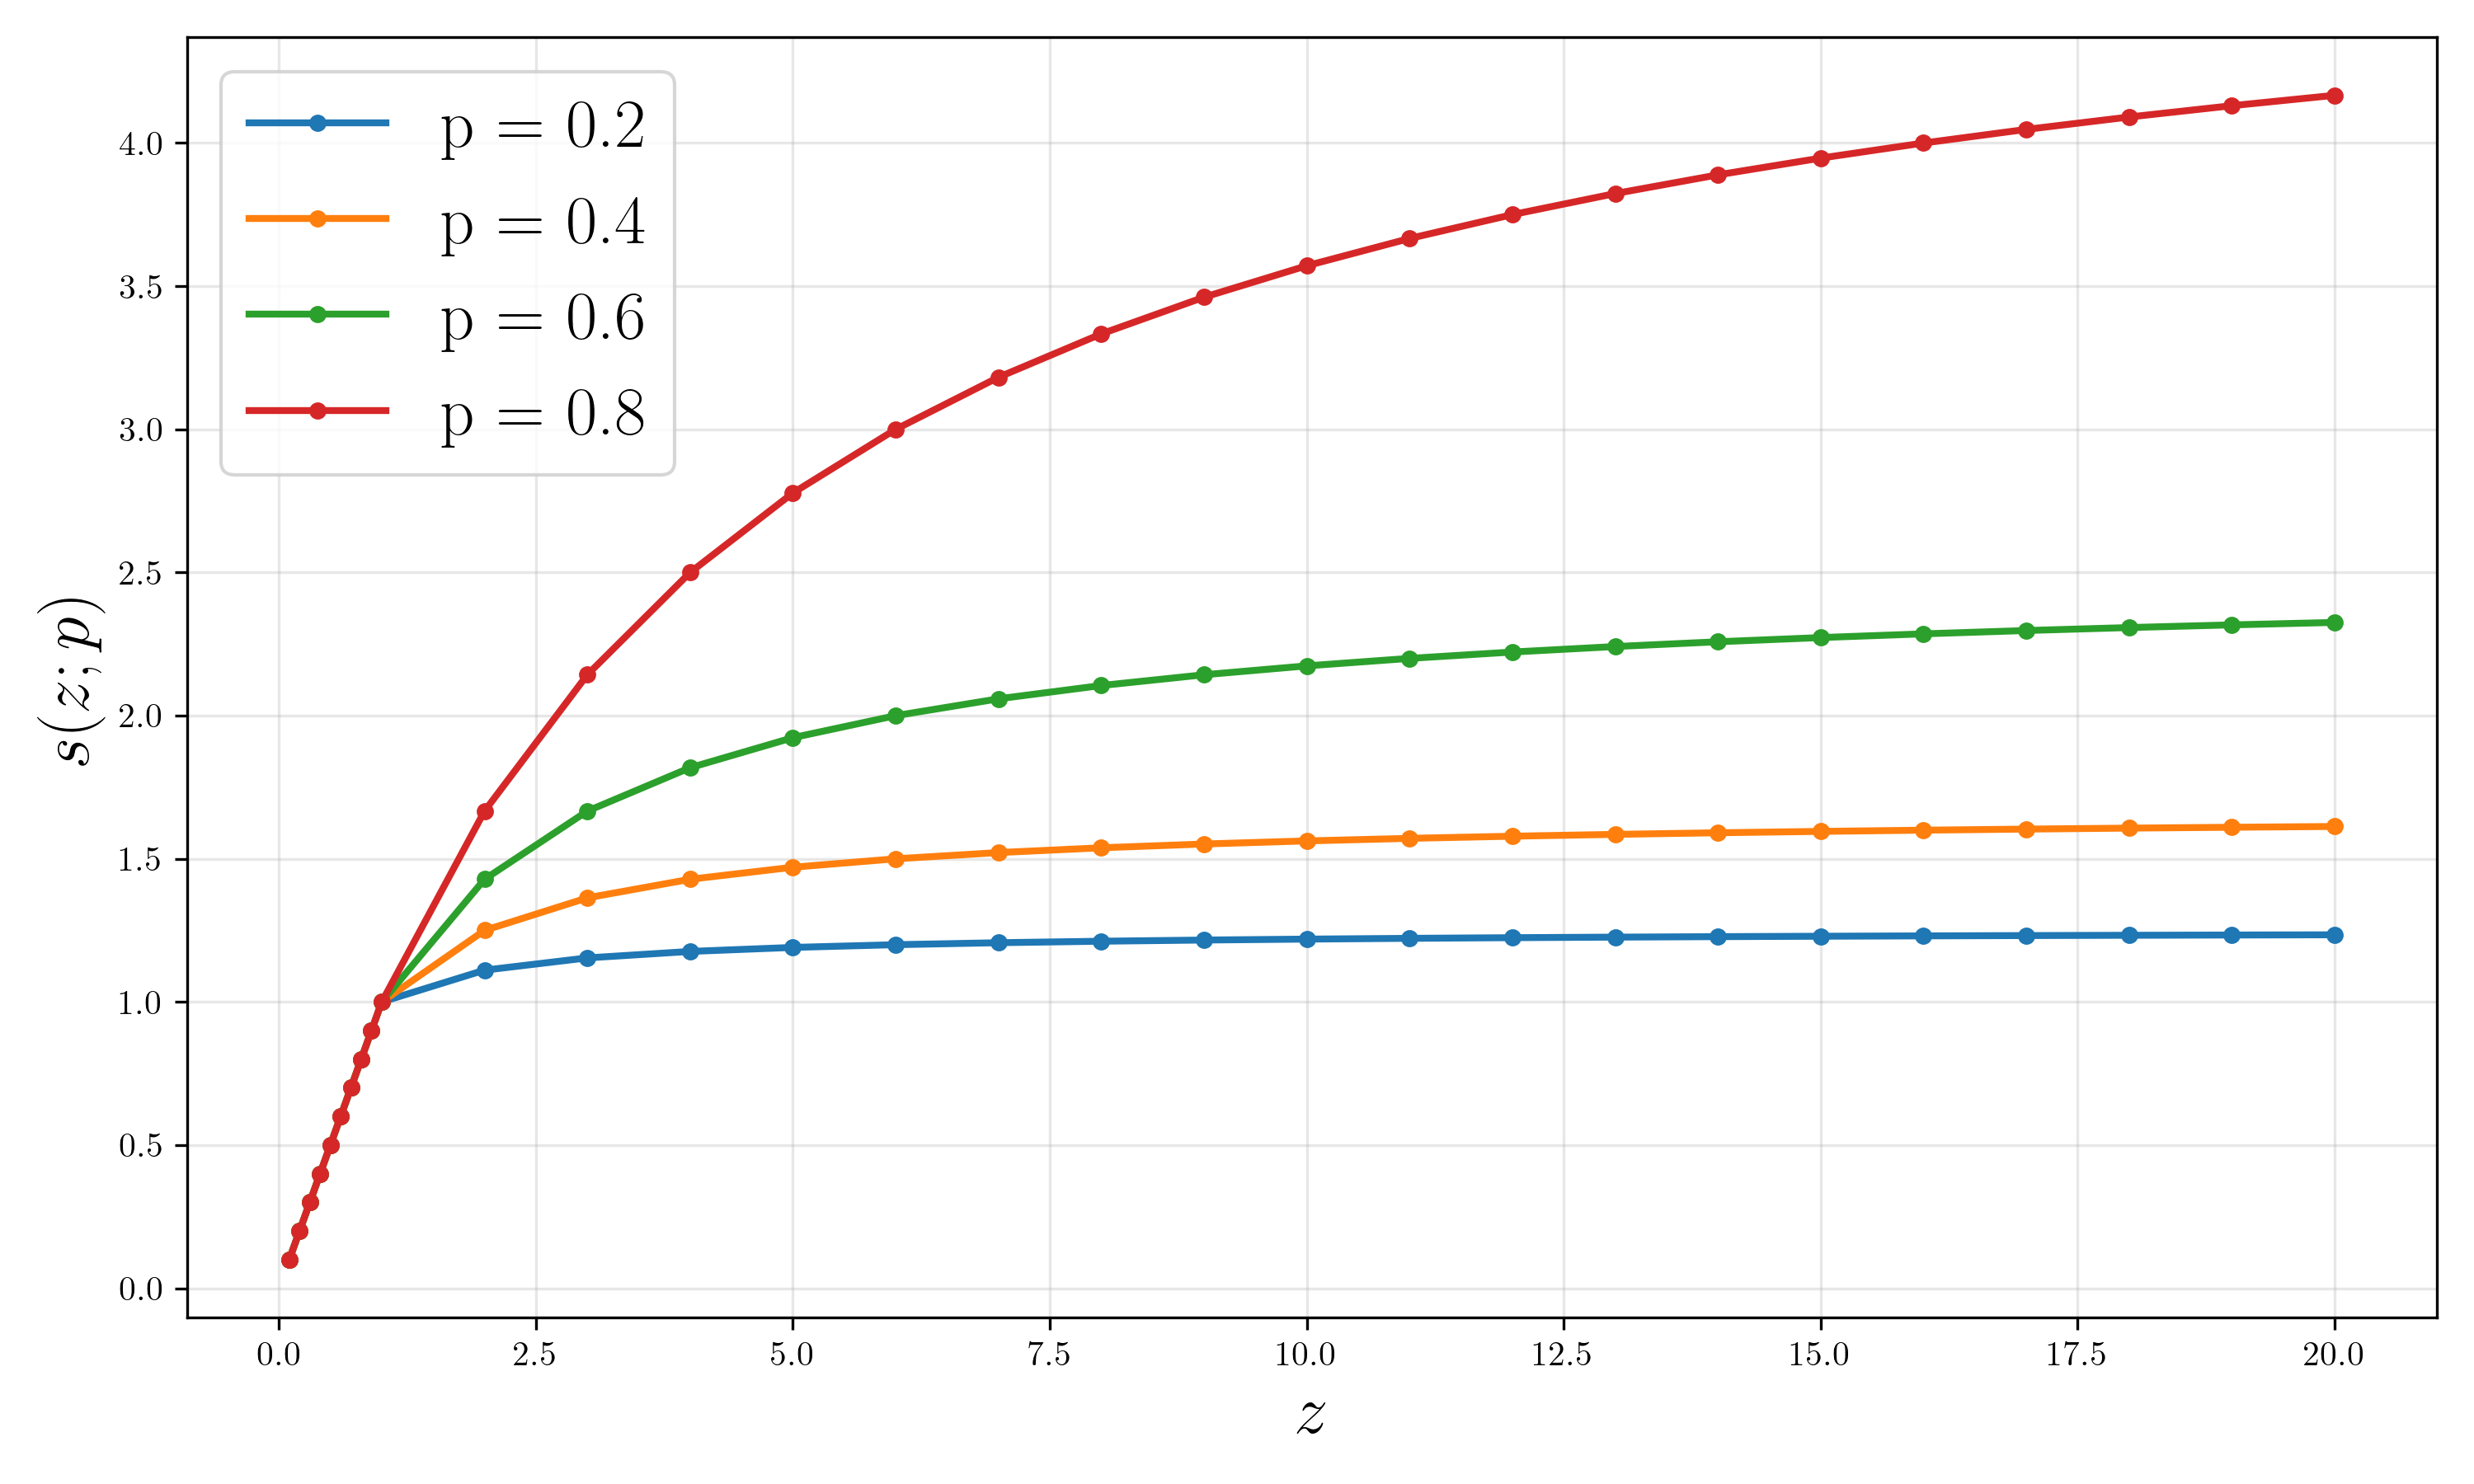
\includegraphics[width=\linewidth]{Images/speed_up_sensitivity_1.png}
        \caption{$s(z;p)$ versus $z$ for Example \ref{example: speed up: amdahl law}}
        \label{fig: Speed up 1}
    \end{subfigure}
    \hfill
    \begin{subfigure}{0.45\textwidth}
        \centering
        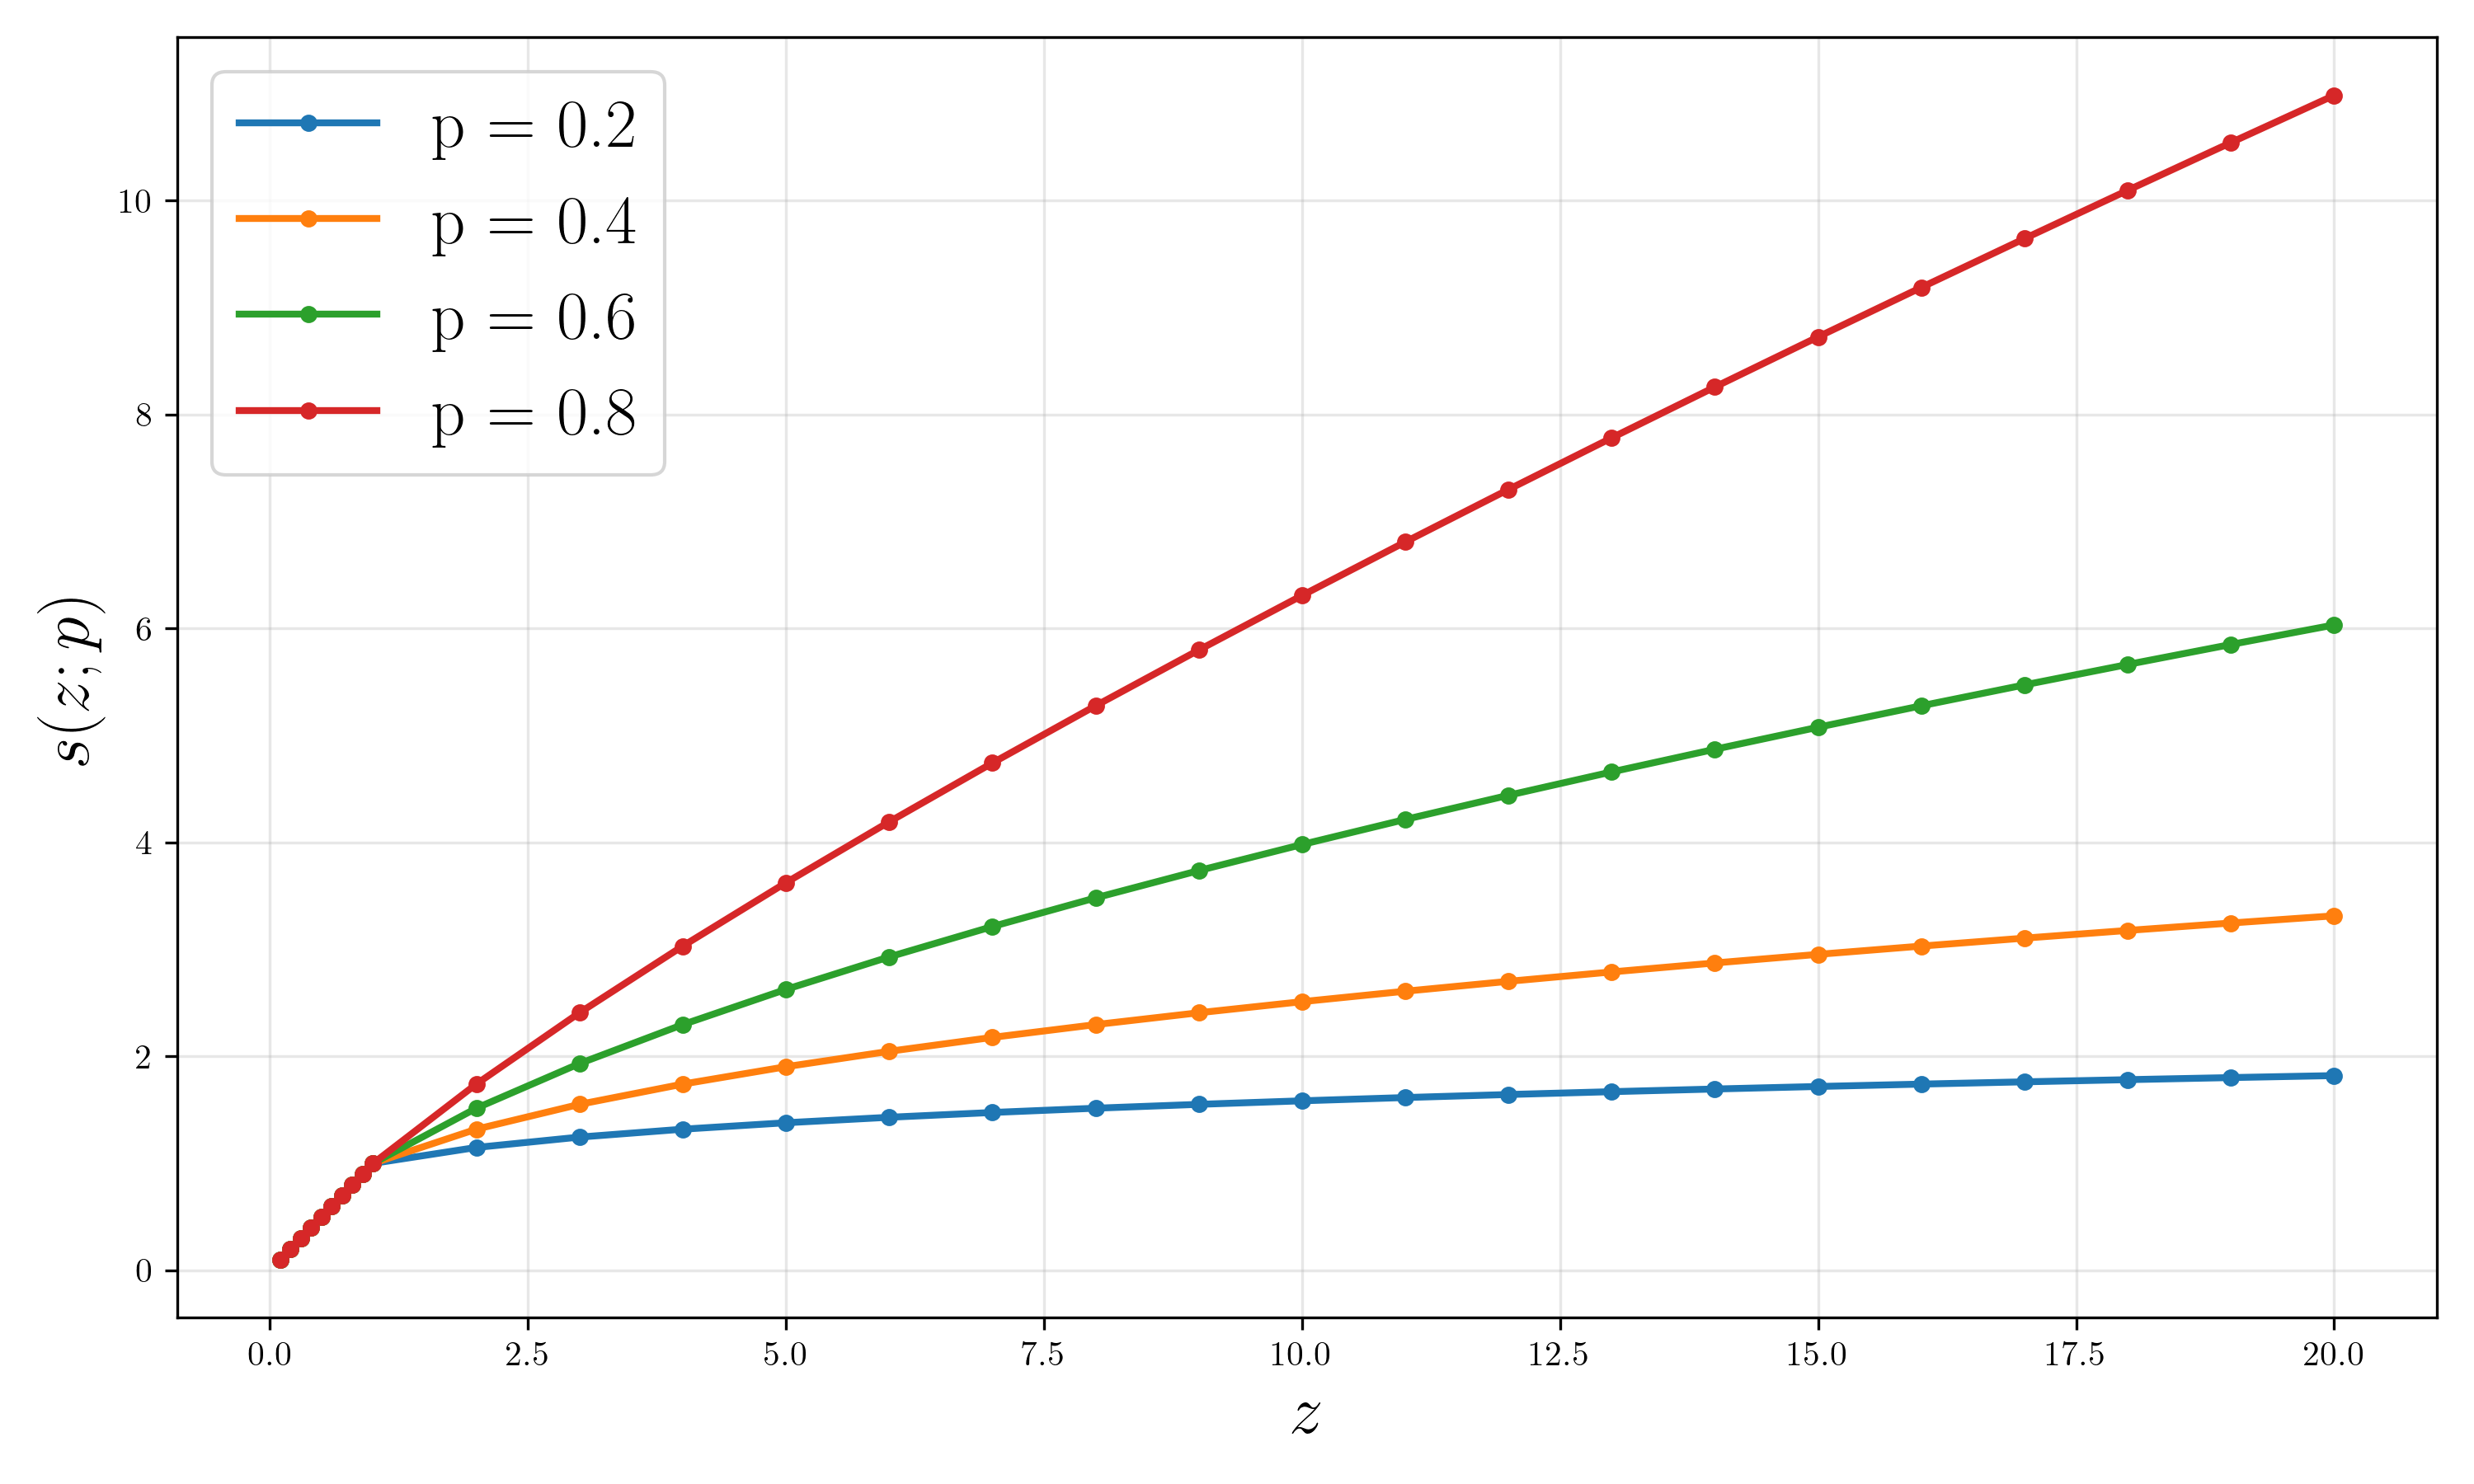
\includegraphics[width=\linewidth]{Images/speed_up_sensitivity_2.png}
        \caption{$s(z;p)$ versus $z$ for Example \ref{example: speed up: 2}}
        \label{fig: Speed up 2}
    \end{subfigure}
    \caption{Plots of example speed-up functions}
    \label{fig:speed up functions}
\end{figure}
% \footnote{\textcolor{blue}{LR: Most instances use \textit{speed-up}, so this should be made consistent (check other places).}}
% \jp{In the figure, it makes no sense to have fractional value labels on the z-axis, if z is assumed integer at all times.}

\begin{remark}
Note that in Example~\ref{example: speed up: amdahl law} as well as in Example~\ref{example: speed up: 2}, $p=0$ corresponds to the case in which jobs are not parallelizable, since $s(z;0)=1$ implies that there is no gain from assigning more than one core to a job. In contrast, $p=1$ yields $s(z;1)=z$ for $z>1$, corresponding to a linear speed-up in the number of allocated cores. In practice, $p$ is expected to lie strictly between these extremes, reflecting positive but diminishing marginal gains from additional cores.\hfill $\spadesuit$
\end{remark}

For a detailed discussion on speed-up functions, we refer the reader to \cite{berg2017}. Next we state an assumption that we impose on the speed-up functions, the reason for which is discussed in Remark \ref{remark:lipschitz} below.

\begin{ass}\label{ass:Lipschitz speed up}
    $s_i(z;\cdot): [0,1] \mapsto \mathbb{R}_+$ is a Lipschitz function, i.e., for all $i \in \{1,2\}$, $z \in [0, c], \ p', p'' \in [0,1]$, there exists $\kappa > 0$ such that $\big\vert s_i(z;p'') - s_i(z;p') \big\vert \leq \kappa \big\vert p''-p' \big\vert$.
\end{ass}

\begin{remark}[On Assumption \ref{ass:Lipschitz speed up}]\label{remark:lipschitz}
Lipschitz continuity of the speed-up function in the parameter $p$ is a mild regularity condition satisfied by standard parametric models. For example, both Amdahl-type speed-up functions and power-law models of the form $s(z;p)=\max\{z,1\}^p$ are Lipschitz in $p$ on compact domains of $z$ (see below). More generally, this assumption ensures that small changes in $p$ induce controlled variations in the effective service rate, reflecting the smooth variation of job characteristics in practice. It is also instrumental in the proof of Theorem~\ref{theorem:strong consistency}, that states that our proposed estimators for the speed-up parameters are consistent. Importantly, the assumption does not restrict qualitative behavior, but merely rules out pathological cases in which arbitrarily small perturbations in $p$ lead to large changes in processing rates. \hfill $\spadesuit$
\end{remark}

We verify Assumption~\ref{ass:Lipschitz speed up} for Examples~\ref{example: speed up: amdahl law} and \ref{example: speed up: 2}. Notice first that in both Examples, $z \leq 1$ implies that $\big\vert s_i(z;p'') - s_i(z;p') \big\vert = |z - z| = 0$, trivially satisfying the condition. Therefore, let us assume $z > 1$ which is the more interesting case.

In both cases, the speed-up function $s(z;\cdot): [0,1] \to [1,\infty)$ is continuous on $[0,1]$ and differentiable on $(0,1)$. By the mean value theorem, it suffices to show that there exists $\kappa>0$ such that $\big\lvert \nabla_p s(z;p) \big\rvert \le \kappa$ for all $p \in (0,1)$, uniformly in $z$. This constant $\kappa$ then satisfies Assumption~\ref{ass:Lipschitz speed up}. In particular, 
\begin{align*}
    &\text{Example } \ref{example: speed up: amdahl law}:  \nabla_p s(z;p) = \frac{1 - \frac{1}{z}}{\big(1 - p\big(1 - \frac{1}{z}\big)\big)^2} \leq \frac{1 - \frac{1}{z}}{\big(1 - \big(1 - \frac{1}{z}\big)\big)^2} = \frac{1 - \frac{1}{z}}{\big(\frac{1}{z}\big)^2} = z^2 - z \leq c^2 - c =: \kappa.
    \\
    &\text{Example } \ref{example: speed up: 2}: \nabla_p s(z;p) = z^p \log z \leq z \log z 
    \leq c \log c =: \kappa.
\end{align*}

% We further assume that jobs are {\it malleable}, i.e.\ the number of servers assigned to them can change at any point in their service.
% Malleability is a natural assumption in the context of dynamic resource allocation, as it enables the system to continuously adapt resource assignments in response to changing system conditions and improved estimates of speed-up parameters.
% Such flexibility is essential in our setting, where allocation decisions are updated over time based on observed performance. 
% Moreover, malleability is supported by modern parallel computing frameworks and cluster management systems, where applications can dynamically acquire and release processing resources during execution \cite{cera2010, gupta2014, delimitrou2014}. 
% While this assumption introduces additional modelling flexibility compared to rigid or moldable jobs, it provides a tractable and practically relevant abstraction for studying adaptive resource allocation in large-scale computing environments.


% \jp{18mar, again the reader may have questions. Why these assumptions? Are they natural? Needed for analysis? What if we don't have these assumptions. These questions will need to be addressed, either here or somewhere earlier.}

\subsection{Objective}
% In this paper, a {\it core allocation policy} is a function
% \begin{align*}
%     \pi: \{0, 1, \cdots, n_{\max}\} \times \{0, 1, \cdots, n_{\max}\} \mapsto \{0,1,\cdots,c\},
% \end{align*}
% which maps the pair $(n_1, n_2)$ (where $n_i$, for $i = 1,2$ is the number of category $i$ jobs in the system) to $\pi(n_1,n_2)$ which is the integral number of servers between $0$ and $c$ (including both end-points) to the category 1 jobs.
% % \jp{Number of servers allocated you mean? What do you mean with inclusive?}
% This automatically implies that $c - \pi(n_1,n_2)$ many servers are allocated to the category 2 jobs.
% We further assume that the servers within each job category are equally divided amongst the jobs within that category, i.e., for $n_1, n_2 > 0$, each category 1 job receives $\pi(n_1, n_2)/n_1$ many servers, and each category 2 job receives $\big(c-\pi(n_1, n_2)\big)/n_2$ many servers.
% Such a policy falls under the class EQUI.
% Reference \cite{berg2017} shows that EQUI is optimal when minimizing the mean number of jobs in the system when all jobs follow a single speed-up curve and have exponentially distributed inherent sizes. 
In this paper, a {\it core allocation policy} is a function
\begin{align*}
\pi: \mathbb{Z} \times \mathbb{Z} \to [0,1],
\end{align*}
which maps the state $(n_1,n_2)$, where $n_i$ denotes the number of class-$i$ jobs in the system, to the fraction $\pi(n_1,n_2)$ of cores allocated to class~1. The remaining fraction $1-\pi(n_1,n_2)$ of cores are assigned to class~2.
% The policy space can be chosen to be the continuous interval $[0,1]$ instead of $\{0, 1/c, \ldots, 1\}$.
% However, purely for ease of computation in the optimization step of Equation \eqref{eqn: defn: H} which we encounter in Section \ref{section: numerical experiments}, we choose $\{0, 1/c, \ldots, 1\}$.
Within each class, cores are divided equally among the active jobs: for $n_1,n_2>0$, each class-1 job receives $c\pi(n_1,n_2)/n_1$ cores, and each class-2 job receives $c(1-\pi(n_1,n_2))/n_2$ cores. Policies of this form belong to the class {\sc equi} (equal sharing) policies.
It is shown in \cite{berg2017} that {\sc equi} is optimal for minimizing the mean number of jobs in the system when all jobs share a common speed-up curve and have exponentially distributed service requirements,{as is the case in our model.}
% \jp{18mar, optimal in regards to what? You haven't talked about objective functions yet.}
% \jp{I wouldn't start a sentence with a reference like this. Also, maybe a numerical example to illustrate everything may go a long way for the reader? It'd be nice if it could be a running example you could use to exemplify things later on to. You can also use it to explain e.g. why you allow $x$ to be fractional $s(x; p_i)$?}


In this paper, our objective is to learn a policy $\pi^*$ that minimizes the mean response time  of jobs in the system.
% \footnote{\textcolor{blue}{LR: Is response time better for this kind of paper?}}
By Little’s law, this is equivalent to minimizing the mean number of jobs in steady state.
Let $\Pi$ denote the class of policies that  prevents starvation of either job class, and ensures that the system is a regenerative process\footnote{\textcolor{blue}{LR: We may need to add an identifiability condition here that ensures that the departure rates depend on $p_i$ in a meaningful way.}}. {Concretely, this means that policies which assign all cores to one job class, when there are only jobs of the other jobs class are present, are not considered}.
% \footnote{LR: What is wrong with a policy that sometimes allocates zero cores to one of the types? E.g., $\pi(n_1,n_2)=c$ for $n_2<M<n_{\max}$ and $\pi(n_1,n_2)<c$ for $n_2\geq M$ - this avoids starvation, right? MM: I am a but confused about whether or not we allow fractional shares of the service capacity.}
% \begin{align}\label{defn:feasible_policy_space}
% \Pi := \big\{\pi \ \big|\ \pi(n_1,n_2) = 0 \ \text{if } n_1 = 0,\ \pi(n_1,n_2) = 1 \ \text{if } n_2 = 0, n_1 > 0 \big\}.
% \end{align}
% \footnote{\textcolor{red}{SAB: Check again}}
For a policy $\pi \in \Pi$, let $N^{\pi}_1$ and $N^{\pi}_2$ denote the stationary numbers of class-1 and class-2 jobs in the system. The optimal policy is then defined as
\begin{align*}
\pi^* := \arg\min_{\pi \in \Pi} \mathbb{E}_{\pi}\big[N^{\pi}_1 + N^{\pi}_2\big].
\end{align*}



\subsection{Learning algorithm}\label{subsection: model description: learning algorithm}
In this subsection, we provide a high-level overview of the algorithm developed in this paper for learning $\pi^*$. 
For $k \geq 1$, it identifies the policy $\pi_k$ that is run between times $\widetilde T_{k-1}$ and $\widetilde T_k$ (here, $\widetilde{T}_0 := 0$), for a duration $T_k:= \widetilde T_k-\widetilde T_{k-1}$. 
The sequence $\big\{\widetilde{T}_k\big\}_{k \geq 1}$ is a sequence of random variables whose construction is described in Section \ref{section: numerical experiments}.
In the algorithm below $n_{\rm steps}$ denotes the number of times we adapt the policy.
\begin{algorithm}[H]
\caption{High-level solution outline}
\label{alg: high level outline}
\begin{algorithmic}[1]
\State Given: $\lambda, \mu, c, s_1(\cdot;\cdot), s_2(\cdot;\cdot)$, sequence $\big\{\widetilde{T}_k\big\}_{k \geq 1}$, $\pi_1 \in \Pi$;
\For{$k = 1,2,\dots, n_{\text{steps}}$}
\State Run the system under policy $\pi_k$ during $\big[\widetilde{T}_{k-1}, \widetilde{T}_k\big)$;
\State Store all arrival and departure times in $\bs{Z}_k$;
\State Using a MLE procedure on $\bs{Z}_k$, to obtain estimators $\big(\widehat{p}_{1,k+1}$,$\,\widehat{p}_{2,k+1}\big)$ for $(p_1, p_2)$;
\State Solve Bellman optimality equation using $\big(\widehat{p}_{1,k+1}$,\,$\widehat{p}_{2,k+1}\big)$ to obtain policy $\pi_{k+1}$;
\EndFor
\State Output: $\pi_{n_{\rm steps}+1}$;
\end{algorithmic}
\end{algorithm}

% For any set of fixed parameters, the optimal core allocation policy can be evaluated by solving the Bellman optimality equation corresponding to the Markov Decision Process (MDP) which is obtained by modelling the system in discrete-time.
% This is discussed in detail in Section \ref{section: optimal policy}.
% Therefore, clearly, the core goal of this paper really is to get refined estimators $\big(\widehat{p}_1, \widehat{p}_2\big)$ for $(p_1, p_2)$, so that we can we can then obtain the optimal core allocation policy.
% Section \ref{section: estimation procedure} describes a maximum likelihood estimation (MLE) procedure which uses the departure process data to obtain these estimators.
% By making an appropriate choice for the sequence $\big\{\widetilde{T}_k\big\}_{k \geq 1}$, these estimators keep getting refined, and eventually converge to $(p_1, p_2)$.
% Section \ref{section: Learning Algorithm} describes the complete algorithm to learn the optimal core allocation scheme. 

For any fixed parameter values, the optimal core allocation policy can be obtained by solving the Bellman optimality equation associated with the corresponding Markov decision process (MDP), obtained by modelling the system in discrete time. This is detailed in Section~\ref{section: optimal policy}. Hence, the central challenge of this paper is to accurately estimate the unknown parameters $(p_1,p_2)$, since these estimates directly determine the computed optimal policy.

Algorithm~\ref{alg: high level outline} implements this idea in an iterative learning-and-optimization loop. The system is run over successive time intervals under the current policy $\pi_k$, and the resulting sample path data is used to update parameter estimates via a maximum likelihood estimation (MLE) procedure (see Section~\ref{section: estimation procedure}). These updated estimates $\big(\widehat{p}_{1,k+1}, \widehat{p}_{2,k+1}\big)$ are then used to recompute the optimal policy by solving the corresponding Bellman equation, yielding $\widehat{\pi}_{k+1}$.
By an appropriate choice of the update times $\big\{\widetilde{T}_k\big\}_{k \ge 1}$ which is discussed in Section \ref{section: numerical experiments}, the estimators are progressively refined and converge to the true parameters $(p_1,p_2)$, leading to increasingly accurate policy updates. 
Section~\ref{section: numerical experiments} presents the full learning procedure in detail along with numerical experiments which guarantee that it works in practice.


% \begin{remark}
%     The system under consideration is stable, i.e., it has a finite regeneration cycle length.
%     This is because of the cap $n_{\max}$ on the maximum number of type 1 and type 2 jobs each that the system can hold at any given time.
% \end{remark}\jp{Ahh, this explains an earlier question of mine. Can't you just go with the conventional stability conditions? $(\lambda_1+\lambda_2) E[B] < 1$. This is the stability condition you would use when not parallelising, and from the point of efficiency from the server, you cannot do better anyway.}



% \jp{18mar, is the lack of chronological order intentional here? The iterative nature of your algorithm should perhaps be explained in the  earlier sections, or a separate (sub)section, rather than here.}


% To solve this problem, the following two steps are crucial - (a)~estimation, and (b)~exploitation.
% In the estimation step, given a sample path data of the system, we perform maximum likelihood estimation to obtain estimators $\widehat{p}_1, \widehat{p}_2$ for the speed-up parameters $p_1, p_2$.
% In the exploitation step, given the estimators, we model the system as a discrete-time Markov chain and solve the Bellman optimality equation to get the optimal core allocation policy corresponding to the estimated values of the speed-up parameters.
% Our solution to this problem is an iterative estimation and exploitation algorithm.
% In the following two sections, we explore the estimation and exploitation steps which will be pieced together to give the complete algorithm in Section \ref{section: Learning Algorithm}.







\section{Estimation procedure} \label{section: estimation procedure}

In this section, we provide a full description of the estimation procedure for the speed-up parameters $p_1$ and $p_2$. The method is based on a maximum likelihood approach applied to the inter-departure times of jobs.
The key observation we rely on is that the departure process of jobs, of both types, is a state-dependent Poisson process, with a rate determined by the current system state and the allocation policy. 

For $i \in \{1, 2\}$, consider the departure process of class-$i$ jobs.
Fix two consecutive departure epochs of class-$i$ jobs and consider the interval between them. By construction, no class-$i$ departures occur in this interval, but arrivals of both job classes and departures of the other job class may occur.
The system state is fully described by $\big(n^{(i)},c^{(i)}\big)$, where $n^{(i)}$ is the number of class-$i$ jobs and $c^{(i)}$ the total number of cores allocated to them. Conditional on this state, the instantaneous departure rate of class-$i$ jobs is
% \footnote{\textcolor{blue}{LR: Perhaps we should spell out explicitly what happens when $n^{(i)}=0$? This is also important in the likelihood function where we need to replace all such states in the sample path by a 1 (indicator function $\mathbf{1}\{n^{(i)}=0\}$?).}}
\begin{align*}
n^{(i)} \mu\, s_i\left(\frac{c^{(i)}}{n^{(i)}}; p_i\right).
\end{align*}
We assume the allocation policy is known and deterministic, so that after each event of type (arrival or departure of either class), the updated allocation $c^{(i)}$ is uniquely determined by the new system state. Consequently, the pair $\big(n^{(i)},c^{(i)}\big)$, and hence the departure rate, is known at all times. 
It follows that the inter-departure interval can be decomposed into subintervals on which $\big(n^{(i)},c^{(i)}\big)$ is constant, hence the departure rate remains constant on each subinterval. 
Therefore, for a given sequence of departure and arrival events, the likelihood of a class-1 job inter-departure time is given by a product of probabilities that no event occurred during the relevant subinterval and the instantaneous exponential density at the actual departure time. 
This form resembles an inhomogeneous Poisson process with piecewise constant rates.
In the remainder of the section, we mathematically formalize the above intuitive description and construct the maximum likelihood estimation procedure to estimate $p_1, p_2$, using the state-dependent departure rates. We then state and prove a theorem which assures strong consistency of the maximum likelihood estimators.

\begin{remark}\label{rem:dep_estimators}
     Note that while the estimation procedures of both parameters $(p_1,p_2)$ are dependent as they rely on the same data, they can be seen as parallel processes with an identical construction. In particular, the following consistency analysis applies to each estimator separately. In fact, this procedure can be  implemented to any number of job classes by considering the departure process of every class individually. \hfill $\spadesuit$
\end{remark}

% Let $i \in \{1, 2\}$ be the job-category.
% Let $\left\{\widetilde{D}^{(i)}_j\right\}_{j \geq 1}$ be the departure time sequence of type $i$ jobs, and $\left\{D^{(i)}_j\right\}_{j \geq 1}$ the corresponding inter-departure times, i.e.\ $D^{(i)}_j = \widetilde{D}^{(i)}_{j+1} - \widetilde{D}^{(i)}_j$.
% Let $N^{(i)}_{\text{d}}(.)$ denote the counting process of type $i$ departures.
% Let ${\mathscr N}^{(i)}_{j,t} := N_{e}\left(\widetilde{D}^{(i)}_j, \widetilde{D}^{(i)}_j+t\right]$ be the number of events (an arrival or departure of a job of any type) in the interval $\left(\widetilde{D}^{(i)}_j, \widetilde{D}^{(i)}_j+t\right]$, with the corresponding event times being denoted in the manner $E^{(i)}_{j,1}, \cdots, E^{(i)}_{j,{\mathscr N}^{(i)}_{j,t}}$. 
% % \textcolor{blue}{(SAB: I think the +1 here, and as a result everywhere henceforth has to be removed. Something to check later.)}
% Let $\left\{\left(n^{(i)}_{j,k}, c^{(i)}_{j,k}\right)\right\}_{k = 1}^{{\mathscr N}^{(i)}_{j,t}+1}$ be the collection of pairs: number of type $i$ jobs, corresponding number of servers allocated to these jobs in the $\Big({\mathscr N}^{(i)}_{j,t}+1\Big)$-many sub-intervals $\left(\widetilde{D}^{(i)}_j, E^{(i)}_{j,1} \right], \left(E^{(i)}_{j,1}, E^{(i)}_{j,2}\right], \cdots, \left(E^{(i)}_{j,{\mathscr N}^{(i)}_{j,t}}, \widetilde{D}^{(i)}_j + t\right]$ respectively.
% For compactness of notation, let us define $\varphi^{(i)}_{j,k} := c^{(i)}_{j,k}/n^{(i)}_{j,k}$.
% Then, relying on standard properties of a non-homogeneous Poisson process, the number of type $i$ departures in the interval $\Big(\widetilde{D}^{(i)}_j, \widetilde{D}^{(i)}_j + t\Big]$, denoted by $N^{(i)}_{\text{d}}\Big(\widetilde{D}^{(i)}_j, \widetilde{D}^{(i)}_j + t\Big]$ is distributed as  

% % \textcolor{magenta}{Proposal for compact notation: for instance, when defining
% % \[\varphi^{(i)}_{j,k}:=\frac{c^{(i)}_{j,k}}{n^{(i)}_{j,k}},\quad {\mathscr N}^{(i)}_{j,t}:=N_{e}\big(\widetilde{D}^{(i)}_j, \widetilde{D}^{(i)}_j + t\big]\]
% % everything becomes significantly more `parsable' and transparent.}

% \jp{An example with numerical sample path and picture may also help for the reader to parse. This is quite a heavy bit of notation to parse in one go. Perhaps some notation needs to move to Section 2 too? I would also, instead of $x^i$ propose $x^{(i)}$ to avoid confusion with powers.}
% \begin{align}
%     &N^{(i)}_{\text{d}}\Big(\widetilde{D}^{(i)}_j, \widetilde{D}^{(i)}_j + t\Big] \notag
%     \\
%     &\sim \text{Poisson} \ \Bigg(
%         \int_{\widetilde{D}^{(i)}_j}^{E^{(i)}_{j,1}} n^{(i)}_{j,1} \ \mu \, s\left(\varphi^{(i)}_{j,1} ; p_i\right) \mathrm{d}t
%         + \int_{E^{(i)}_{j,1}}^{E^{(i)}_{j,2}} n^{(i)}_{j,2} \ \mu \, s\left(\varphi^{(i)}_{j,2}; p_i\right) \mathrm{d}t + \cdots \notag
%     \\
%     &\hspace{2cm} + \int_{E^{(i)}_{j,{\mathscr N}^{(i)}_{j,t}}}^{\widetilde{D}^{(i)}_j + t}
%         n^{(i)}_{j, {\mathscr N}^{(i)}_{j,t}+1} \ \mu \,
%         s\left(
%             \varphi^{(i)}_{j, {\mathscr N}^{(i)}_{j,t}+1};p_i
%         \right) \mathrm{d}t
%     \Bigg) \notag
%     \\ 
%     &=\;\text{Poisson} \ \Bigg(
%         \mu \Bigg[
%             n^{(i)}_{j,1} s\left(\varphi^{(i)}_{j,1}; p_i\right)\Big(E^{(i)}_{j,1} - \widetilde{D}^{(i)}_j\Big)
%             + n^{(i)}_{j,2} s\left(\varphi^{(i)}_{j,2}; p_i\right)\Big(E^{(i)}_{j,2} - E^{(i)}_{j,1}\Big) + \cdots \notag
%     \\
%     &\hspace{2cm}
%         + \ n^{(i)}_{j, {\mathscr N}^{(i)}_{j,t}+1}
%         \ s\left(
%             \varphi^{(i)}_{j, {\mathscr N}^{(i)}_{j,t}+1}; p_i
%         \right)
%         \bigg(\widetilde{D}^{(i)}_j + t - E^{(i)}_{j, {\mathscr N}^{(i)}_{j,t}}\bigg)
%         \Bigg] \Bigg).
% \end{align}
Once again, let $i \in \{1,2\}$ denote the job class. 
Define $\widetilde{D}^{(i)}_0 := 0$, and let $\Big\{\widetilde{D}^{(i)}_j\Big\}_{j \ge 1}$ be the departure epochs of type-$i$ jobs, with inter-departure times
\[
D^{(i)}_j := \widetilde{D}^{(i)}_{j} - \widetilde{D}^{(i)}_{j-1}, \ j \geq 1.
\]
Every such inter-departure interval can be split into subintervals corresponding to \textit{`rate changing events'}. 
Specifically, for $j \geq 1$, let
\[\Big\{E^{(i)}_{j,k}\Big\}_{k=1}^{\mathscr N^{(i)}_{j}}\] denote the event times (arrivals of any job class or departures of the non-$i$ job class), where $\mathscr N^{(i)}_{j}$ is the total number of events occurring in $\Big(\widetilde{D}^{(i)}_{j-1}, \widetilde{D}^{(i)}_{j}\Big)$. 
Then,
\[
\left[\widetilde{D}^{(i)}_{j-1},\widetilde{D}^{(i)}_{j}\right)= \underbrace{\left[\widetilde{D}^{(i)}_{j-1}, E^{(i)}_{j,1}\right)}_{\text{Interval 1}} \cup \underbrace{\left[E^{(i)}_{j,1}, E^{(i)}_{j,2}\right)}_{\text{Interval 2}} \cup  \ldots \cup \underbrace{\left[E^{(i)}_{j,\mathscr N^{(i)}_{j}}, \widetilde{D}^{(i)}_{j}\right)}_{\text{Interval } \mathscr N^{(i)}_j+1}.
\]
Further for $k \in \big\{1, \cdots, \mathscr{N}^{(i)}_j+1\big\}$, let $\Big(n^{(i)}_{j,k}, c^{(i)}_{j,k}\Big)$ be the number of type-$i$ jobs and allocated cores in the $\big(\mathscr N^{i}_j+1\big)$ intervals listed above.
Understand that this pair remains fixed within each of these intervals.
Figure~\ref{fig:departure times} and Figure~\ref{fig:event times} assist the reader in visualizing these notations.

\begin{figure}[htbp]
    \centering
    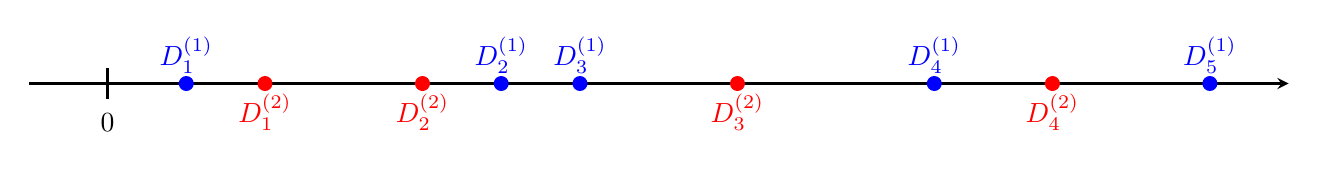
\begin{tikzpicture}[>=stealth, thick]
    
    % Time axis
    \draw[->] (0,0) -- (16,0);

    % Endpoints (departures with ticks)
    \draw (1,0.2) -- (1,-0.2);
    \node[below] at (1,-0.25) {0};
    
    % Type 1 departures (blue, on the line)
    \foreach \x/\label in {
        2/$D^{(1)}_1$,
        6/$D^{(1)}_2$,
        7/$D^{(1)}_3$,
        11.5/$D^{(1)}_4$,
        15/$D^{(1)}_5$
    }
    {
        \filldraw[blue] (\x,0) circle (2.3pt);
        \node[above, blue] at (\x,0) {\label};
    }
    
    % Type 2 departures (red, same line)
    \foreach \x/\label in {
        3/$D^{(2)}_1$,
        5/$D^{(2)}_2$,
        9/$D^{(2)}_3$,
        13/$D^{(2)}_4$
    }
    {
        \filldraw[red] (\x,0) circle (2.3pt);
        \node[below, red] at (\x,0) {\label};
    }
    
    \end{tikzpicture}
    \caption{Departure epochs of class-1 (blue) and class-2 (red) jobs on a single timeline.}
    \label{fig:departure times}
\end{figure}

\begin{figure}[htbp]
\centering
    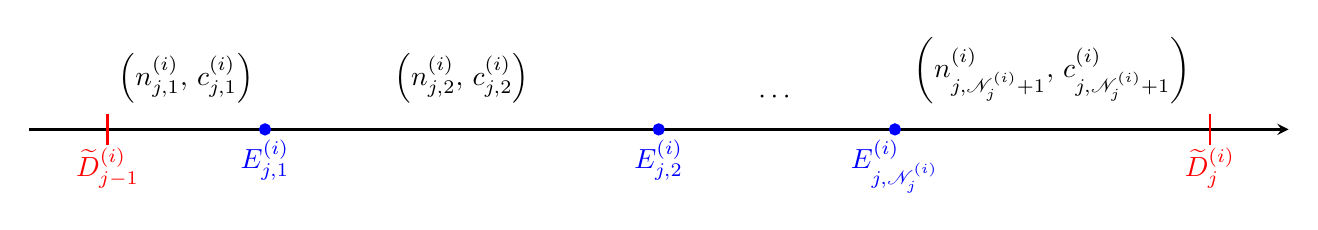
\begin{tikzpicture}[>=stealth, thick]
    
    % Timeline
    \draw[->] (0,0) -- (16,0);
    
    % Endpoints (departures with ticks)
    \draw[red] (1,0.2) -- (1,-0.2);
    \node[below, red] at (1,-0.1) {$\widetilde{D}^{(i)}_{j-1}$};
    
    \draw[red] (15,0.2) -- (15,-0.2);
    \node[below, red] at (15,-0.1) {$\widetilde{D}^{(i)}_{j}$};
    
    % Event points (solid dots, nicely spaced)
    \foreach \x/\label in {
        3/$E^{(i)}_{j,1}$,
        8/$E^{(i)}_{j,2}$,
        11/$E^{(i)}_{j,\mathscr N^{(i)}_{j}}$
    }
    {
        \filldraw[blue] (\x,0) circle (1.8pt);
        \node[below, blue] at (\x,0) {\label};
    }
    
    % Interval labels (states)
    \node[above] at (2,0.2) {$\left(n^{(i)}_{j,1},\,c^{(i)}_{j,1}\right)$};
    \node[above] at (5.5,0.2) {$\left(n^{(i)}_{j,2},\,c^{(i)}_{j,2}\right)$};
    \node[above] at (9.5,0.2) {$\cdots$};
    \node[above] at (13,0.2) {$\left(n^{(i)}_{j,\mathscr N^{(i)}_{j}+1},\,c^{(i)}_{j,\mathscr N^{(i)}_{j}+1}\right)$};
    
    \end{tikzpicture}
    \caption{Inter-departure time of class-$i$ jobs decomposed into sub-intervals with constant state.}
    \label{fig:event times}
\end{figure}



Define the per-job allocation ratio, which is the number of cores allocated per job, during interval $k=1,\ldots,\mathscr N^{(i)}_{j}+1$ as
\[
\varphi^{(i)}_{j,k} := \frac{c^{(i)}_{j,k}}{n^{(i)}_{j,k}}.
\]
Then the departure rate $\delta^{(i)}_{j,k}$ of class-$i$ jobs during interval $k=1,\ldots,\mathscr N^{(i)}_{j}+1$ is given by
\begin{align*}
    \delta^{(i)}_{j,k} = 
    \begin{cases}
        n^{(i)}_{j,k} \, \mu \, s_i\Big(\varphi^{(i)}_{j,k};p_i\Big), &n^{(i)}_{j,k} > 0,
        \\
        0, &n^{(i)}_{j,k} = 0.
    \end{cases}
\end{align*}

Let $\xi_k$ denote the probability of no class-$i$ departure during the interval $k=1,\ldots,\mathscr N^{(i)}_{j}$.
Then,
\begin{align*}
    \xi_k=\left\lbrace\begin{array}{cc}
        \exp\biggl(-\delta^{(i)}_{j,k} \Big(E^{(i)}_{j,1} - \widetilde{D}^{(i)}_{j-1}\Big)\biggr),  & k=1, \\
         \exp\biggl(-\delta^{(i)}_{j,k} \Big(E^{(i)}_{j,k} - E^{(i)}_{j,k-1}\Big)\biggr), &  k=2,\ldots \mathscr{N}^{(i)}_{j}.
    \end{array}\right .
\end{align*}
Similarly, the probability of no event\footnote{\textcolor{blue}{LR: Should event be replaced with 'class-i departure'?}} during $\bigg(E^{(i)}_{j,\mathscr N^{(i)}_{j}} ,E^{(i)}_{j,\mathscr N^{(i)}_{j}}+t\bigg]$ is given by
\begin{align*}
    \xi_{\mathscr{N}^{(i)}_{j}+1}(t)= \exp\biggl(-\delta^{(i)}_{j, \mathscr N^{(i)}_j+1} t\biggr), \ t\leq \widetilde{D}^{(i)}_{j}-E^{(i)}_{j,\mathscr N^{(i)}_{j}} .
\end{align*}
Let $\bs \chi$ store the complete sample path evolution of the system, and for convenience, let $\bs\chi\big(t_1, t_2\big]$ be the subset of $\bs\chi$ observed in the interval $\big(t_1, t_2\big]$.
Consequently, the conditional likelihood of the class-$i$ departure process given the observed event sequence $\bs\chi\left(\widetilde{D}^{(i)}_{j-1}, \widetilde{D}^{i}_j\right]$ is
\begin{align}\label{likelihood: one interdeparture time}
    \mathcal{L}\Big(p_i; \bs\chi\left(\widetilde{D}^{(i)}_{j-1}, \widetilde{D}^{i}_j\right]\Big) =    \left(\prod_{k=1}^{\mathscr{N}^{(i)}_{j}}\xi_k  \right) \delta^{(i)}_{j, \mathscr N^{(i)}_j+1} \, \xi_{\mathscr{N}^{(i)}_{j}+1}.
\end{align}
\footnote{\textcolor{blue}{LR: What happens when $n^{(i)}=0$? I think the term in the product should be a 1.}}
This expression is obtained by multiplying
\begin{enumerate}
    \item exponential survival $\xi_{k}$ for $k \in \Big\{1, 2, \cdots, \mathscr{N}^{(i)}_j\Big\}$,over all $\mathscr{N}^{(i)}_j$ preceding sub-intervals, and
    \item the instantaneous hazard at the departure epoch.
\end{enumerate}
Now, suppose our observed system data comprises $M_i$ departures of class $i$. 
Then, the likelihood $\mathcal{L}\big(p_i; \bs\chi\big)$ of the parameter $p_i$ conditioned on $\bs\chi$ and the corresponding log-likelihood $\ell\big(p_i;\bs\chi\big)$ are
\begin{align}
    \mathcal{L}\big(p_i; \bs\chi\big) &= \prod_{j=1}^{M_i} \mathcal{L}\Big(p_i; \bs\chi\left(\widetilde{D}^{(i)}_{j-1}, \widetilde{D}^{i}_j\right]\Big), \; \label{eqn:likelihood}
    \\
    \ell\big(p_i; \bs\chi\big) &= \log\Big( \mathcal{L}\big(p_i; \bs\chi\big) \Big)
    = \sum_{j=1}^{M_i} \log \bigg(\mathcal{L}\Big(p_i; \bs\chi\left(\widetilde{D}^{(i)}_{j-1}, \widetilde{D}^{i}_j\right]\Big)\bigg), \label{eqn:log likelihood}
\end{align}
In particular,
\begin{align}\label{eqn:log_likelihood:formula}
    \ell\big(p_i; \bs\chi\big) = \ &M_i \log(\mu)
    + \sum_{j=1}^{M_i} \log\Bigg(n^{(i)}_{j, {\mathscr N}^{(i)}_{j}+1}\Bigg)
    + \sum_{j=1}^{M_i} \log\left(
    s_i\left(\varphi^{(i)}_{j, {\mathscr N}^{(i)}_{j}+1}; p_i\right)\right)
    \notag
    \\
    &- \mu \sum_{j=1}^{M_i} \Bigg[
    n^{(i)}_{j,1} \ s_i\left(\varphi^{(i)}_{j,1}; p_i\right)\Big(E^{(i)}_{j,1} - \widetilde{D}^{(i)}_{j-1}\Big)
    + \cdots \notag
    \\
    &\hspace{1.5cm}
    + n^{(i)}_{j, {\mathscr N}^{(i)}_{j}+1}
    \ s_i\left(\varphi^{(i)}_{j, {\mathscr N}^{(i)}_{j}+1}; p_i\right)
    \bigg(\widetilde{D}^{(i)}_{j} - E^{(i)}_{j,{\mathscr N}^{(i)}_{j}}\bigg)
    \Bigg].
\end{align}

The MLE of $p_i$, denoted by $\widehat{p}_i$, is then given by
\begin{align} \label{eqn: MLE}
    \widehat{p}_i = \argmax_{p_i \in [0,1]} \ \mathcal{\ell}\big(p_i; \bs\chi\big)
\end{align}

\begin{remark}
    Even though the goal of this section is to jointly estimate $(p_1, p_2)$, \eqref{eqn: MLE} suggests that we can do so by solving two separate optimization problems, one for each $p_1$ and $p_2$.
    However, this does not imply that the estimators $\widehat{p}_1$ and $\widehat{p}_2$ are independent. \hfill $\spadesuit$
    % \jp{Because they are two different datasets? do you mean with independence that these datasets are stochastically independent from one another? If so, this needs an explanation, although I think that's indeed true. It needs an argument on why the fact that $c_1+c_2 = c$ does not make things dependent.}
\end{remark}

\begin{remark}
    The estimation procedure will work for any policy $\pi \in \Pi$.  
    The accuracy of the estimation procedure increases in $M_i$ (the number of observed regeneration cycles in the data), which relates to the specific chosen core allocation policy. \hfill $\spadesuit$
    % \jp{...under the assumption that servers are always allocated whenever there are jobs, in the absence of which you might have a data starvation. Also, the accuracy of the estimation increases with $M_i$, which does relate to the core allocation policy? Definitely something to spell out for the reader.}
\end{remark}

% \jp{This assumption is something to discuss in Section 2, rather than here. I guess usually, we assume the speed-up function to be increasing and sublinear. I guess those two combined with contuinity actually does immediately imply Lipschitz continuity?}

Before stating the result which guarantees strong consistency.
This assumption is made purely to satisfy the requirements of Theorem \ref{theorem:strong consistency} below for strong consistency of the speed-up estimates to their true values.
In particular, it appears in the proof of Lemma \ref{lemma:consistency:andrews} which is a crucial result in the proof of Theorem \ref{theorem:strong consistency} in Section \ref{subsection:proof:theorem:strong consistency}.
Assumption \ref{ass: max jobs} has the role of being able to prove finiteness of expectation of a certain random variable which is a necessity for Lemma \ref{lemma:consistency:andrews}.
However, this assumption is not essential for the methodology designed in this paper to be implemented from a practical point of view.
\begin{ass} \label{ass: max jobs}
    The system is allowed to hold at most $n_{\max}$ number of jobs of each class. That is, any arrival of job type $i$ (for $i = 1,2$) is blocked when there are already $n_{\max}$ number of type $i$ jobs in the system.
\end{ass}
% \jp{18mar, you're referencing forward, so the reader has no way of knowing what Lemma 4.3 or Theorem 4.1 are yet. For the reader this sentence now reads is, 'it's apparently not natural, but made to satisfy some lemmas, and then the sentence says that nevertheless its not essential', which will make no sense. There is a lot more nuance to this, which needs to be conveyed. If this assumption really is not essential, it deserves recommendation to see whether this assumption can be made more locally, because this in a model's section this is a big thing.}

\begin{theorem} \label{theorem:strong consistency}
    Let $0 < \alpha < 1$. Consider an observation of the sample-path of the system under policy $\pi \in \Pi$ with total $n$ jobs. If Assumptions \ref{ass:Lipschitz speed up} and \ref{ass: max jobs} are satisfied, then as $n \rightarrow \infty$, we have $M_1, M_2 \rightarrow \infty$, and $\widehat{p}_1 \overset{\text{a.s.}}{\rightarrow } p_1$, $\widehat{p}_2 \overset{\text{a.s.}} {\rightarrow}p_2$. 
    % \jp{What's $\alpha$? Is this the probability that an arriving job is of class one? It appears nowhere in the proof.}
    % \jp{18mar, while this theorem needs to be phrased a little more verbosely, I think at some point earlier in the paper, there also needs to be a separate subsection on the structure and the idea of your algorithm. While mathematically correct, the reader not completely sure of the general structure of it, may get stuck in esoteric readings of the theorem like 'the phrasing of this theorem implies that as $M_1$ goes to infinity, but $M_2$ stays finite, the estimate for $p_1$ will converge, but $p_2$ might not.' For any sane policy, this will not happen, and there is a joint conversion going on. It may even be a good idea to just introduce an Algorithm 1 in the paper, and provide pseudo-code.}
\end{theorem}
\begin{remark}
    $0 < \alpha < 1$ prevents the degenerate case where the incoming stream of jobs belongs only to one class. \hfill $\spadesuit$
\end{remark}

\subsection{Proof of Theorem \ref{theorem:strong consistency}} \label{subsection:proof:theorem:strong consistency}

In this subsection, we provide the complete proof of Theorem \ref{theorem:strong consistency}.
First, we explain a high-level structure of the proof. 
We start by introducing regeneration cycles in the context of the system under study.
Then, we introduce complex new objects which may seem non-intuitive but will be crucial to the proof of Theorem \ref{theorem:strong consistency}.
Then, Lemma \ref{lemma:consistency:andrews}, and correspondingly Corollary \ref{eqn: andrews_corollary: eqn_1} and \ref{eqn: andrews_corollary: eqn_2} establish certain results which serve as the hypothesis for Theorem \ref{theorem:strong consistency}.
Finally, we use a known result from \cite{andrews1992} to establish the result.

A key ingredient in the proof is the use of \emph{regeneration cycles}, which allow the system’s sample path to be decomposed into independent segments. Exploiting this regenerative structure, we extract i.i.d.\ objects from otherwise dependent queueing data. The availability of such an i.i.d.\ substructure enables us to invoke existing results to establish strong consistency. We refer the reader to \cite{bodas2023} for a detailed exposition of this approach; the analysis presented below is of a similar nature. 
% \jp{18 mar, does this imply that the upcoming proof is mutatis mutandis the same as of [8]? If so, the reader needs to know.}

Let us first define a regeneration cycle in the context of the system under study.
Consider a system that starts empty at time 0.
Then, regeneration time is the first time when there is a departure of a job of either class leading to a fully empty system.

Now, we turn our attention to the creation of i.i.d.\ objects from dependent queueing data, as explained below.
As introduced in Section \ref{section: model description}, consider any fixed policy $\pi: \{0, 1, \cdots, n_{\max}\} \times \{0, 1, \cdots, n_{\max}\} \mapsto [0,1]$.
Then, under policy $\pi$, the system is a regenerative process.
Suppose that the system sample path dataset consists of $N_r$ number of regeneration cycles, where $N_r$ is a random variable (The first and the last may be partial cycles).
% \jp{So $n_{\max}$ is also a random variable?}
% \jp{18mar, there still seems to be a clash in notation between $N_r$ and $n_{\max}$. Is this the point where $n_{\max}$ is needed?}
% \footnote{\textcolor{red}{SAB: $n_{\max} \rightarrow n_{\max}$} make this change.}
Then, we claim that we can decompose the log-likelihood $\ell(p, \bs\chi)$ into a sum of i.i.d.\ random variables as written below.
\begin{align*}
    \ell(p; \bs\chi) = \sum_{k=1}^{N_r} q\big(\bs{Z}_k; p\big).
\end{align*}
Here, for each regeneration cycle $k$,
\begin{align}\label{eqn: Z: state space}
    \bs{Z}_k = \Bigg(C_k, &\Big\{\widetilde{D}^{(i)}_j\Big\}_{j=\widetilde{C}_{k-1}+1}^{\widetilde{C}_k} ,
    \Bigg\{\Big\{n^{(i)}_{j,k}\Big\}_{k=1}^{\mathscr N^{(i)}_{j}+1}\Bigg\}_{j=\widetilde{C}_{k-1}+1}^{\widetilde{C}_k}, 
    \Bigg\{\Big\{c^{(i)}_{j,k}\Big\}_{k=1}^{\mathscr N^{(i)}_{j}}\Bigg\}_{j=\widetilde{C}_{k-1}+1}^{\widetilde{C}_k}, \notag
    \\
    &\Bigg\{\Big\{E^{(i)}_{j,k}\Big\}_{k=1}^{\mathscr N^{(i)}_{j}}\Bigg\}_{j=\widetilde{C}_{k-1}+1}^{\widetilde{C}_k}\Bigg)
    \in \mathscr{Z} := \bigcup_{i=1}^{\infty} \bigcup_{j=1}^{\infty} 
    \Big(\mathbb{N} \times \mathbb{R}^{i}_+ \times \mathbb{N}^{j \times i} \times \mathbb{N}^{j \times i} \times \mathbb{R}_{+}^{j \times i}\Big).
\end{align}
which collects all system information from regeneration cycle $k$. This includes, for instance, the number of class-$i$ job arrivals during cycle $k$, their departure times, the sequence of event times together with the corresponding system states (i.e., the number of jobs present), as well as all core allocations between consecutive event times.
% \jp{18 Mar: The state space could use further clarification. For example, does \eqref{eqn: Z: state space} contain two copies of $\mathcal{R}$, whereas only a single array of $E$’s appears in $\bs{Z}$?}
Furthermore, let $q: \mathscr{Z} \times [0,1] \to \mathbb{R}$ be the function defined in \eqref{eqn:q(Z;p):formula}, and assume that the sequence $\big\{q(\bs{Z}_k; p)\big\}_{k=2}^{N_r-1}$ consists of i.i.d.\ random variables. Recall that cycles $1$ and $N_r$ may be partial regeneration cycles.
For notational simplicity, we consider Equation \eqref{eqn:log_likelihood:formula} without the class index $i$, so that the total number of departures is $M$. Let $C_k$ denote the number of departures (of class-$i$ jobs, with the index suppressed) during the $k$-th regeneration cycle, and define
\[
\widetilde{C}_k := C_1 + \cdots + C_k.
\]
Clearly, $C_k$ also equals the number of arrivals during the $k$-th regeneration cycle, and hence $\widetilde{C}_k$ is the total number of customers that have entered the system over the first $k$ regeneration cycles. For $k \in \{2, \ldots, N_r - 1\}$, we define
\begin{align}\label{eqn:q(Z;p):formula}
    q\big(\bs{Z}_k; p\big) = \ &C_k \log(\mu) 
    + \sum_{j=\widetilde{C}_{k-1}+1}^{\widetilde{C}_k} 
    \log\left(n^{(i)}_{j, {\mathscr N}^{(i)}_{j}+1}\right)
    + \sum_{j=\widetilde{C}_{k-1}}^{\widetilde{C}_k-1}
    \log\left(
    s_i\left(\varphi^{(i)}_{j, {\mathscr N}^{(i)}_{j}+1}; p\right)\right)
    \notag
    \\
    &- \mu \sum_{j=\widetilde{C}_{k-1}}^{\widetilde{C}_k-1} \Bigg[
    n^{(i)}_{j,1} \ s_i\left(\varphi^{(i)}_{j,1}; p\right)
    \Big(E^{(i)}_{j,1} - \widetilde{D}^{(i)}_{j-1}\Big)
    + \cdots \notag
    \\
    &\hspace{1.5cm}
    + n^{(i)}_{j, {\mathscr N}^{(i)}_{j}+1}
    \ s_i\left(\varphi^{(i)}_{j, {\mathscr N}^{(i)}_{j}+1}; p\right)
    \bigg(\widetilde{D}^{(i)}_{j} - E^{(i)}_{j,{\mathscr N}^{(i)}_{j}}\bigg)
    \Bigg].
\end{align}
The definition of $q(\bs{Z}_k;p)$ above has four summands on the right-hand side.
We now verify that each of these summands depends only on data from regeneration cycle $k$, which is crucial for establishing the i.i.d.\ structure across cycles.
% \jp{18 mar: what does "belong explicitly" mean? If it means that $q(z_K, p)$ cannot depend on any data points ouside of this regeneration cycle, shouldn't this already follow immediately by construction/definition from $q(Z_k,p)$? I'm not saying that what you do here is not useful, but the reader needs to be guided on why it's useful.}
\begin{enumerate}

\item \textit{Summand 1.}
This follows directly, since $C_k$ is the number of departures occurring in the $k$-th regeneration cycle.

\item \textit{Summand 2.}
Recall that
\[
n^{(i)}_{j,\mathscr{N}^{(i)}_{j}+1}
\]
is the number of class-$i$ jobs in the interval
\[
\Big( E^{(i)}_{j,\mathscr{N}^{(i)}_{j}},\,\widetilde{D}^{(i)}_{j} \Big],
\]
which is a subinterval of
$
\Big(\widetilde{D}^{(i)}_{j-1},\, \widetilde{D}^{(i)}_{j}\Big].$
Hence, for
$ j = \widetilde{C}_{k-1}+1, \ldots, \widetilde{C}_k-1,$
this interval lies entirely within the $k$-th regeneration cycle.
For $j = \widetilde{C}_{k-1}$, observe that
\[ E^{(i)}_{j,\mathscr{N}^{(i)}_{j}} \]
is the last event before $\widetilde{D}^{(i)}_{j+1}$. Since at least one event — namely the arrival of job $j+1$ — occurs in the $k$-th regeneration cycle, this interval also lies within the $k$-th regeneration cycle.

\item \textit{Summand 3.}
This follows by the same argument as in Summand 2, since it depends on the same quantities.

\item \textit{Summand 4.}
For
\[
j = \widetilde{C}_{k-1}+1, \ldots, \widetilde{C}_k-1,
\]
all quantities in the fourth summand are clearly associated with the $k$-th regeneration cycle.

For $j = \widetilde{C}_{k-1}$, note that if any
$
E^{(i)}_{j,\cdot}
$
lies in the $(k-1)$-th regeneration cycle, then the corresponding
\[
n^{(i)}_{j,\cdot} = 0,
\]
and hence such terms do not contribute.

\end{enumerate}

Now we have introduced all the necessary objects to prove Theorem \ref{theorem:strong consistency}.
Lemma \ref{lemma:consistency:andrews}, and in particular Equations \ \eqref{eqn: andrews_corollary: eqn_1} and \eqref{eqn: andrews_corollary: eqn_2} in Corollary \ref{lemma:consistency:andrews} below, have the purpose of verifying necessary hypothesis for using known results to prove strong consistency.
%\jp{18mar, I guess the reader benefits if you provide the overall structure of the proof first in a couple of lines, and say what Lemma 4.3 does and what its overall purpose is. If the reader does not know the grand picture beforehand, it's easy to get lost in details.}



% \begin{lemma} \label{lemma:consistency:andrews}
%     Let $p \in [0,1]$. 
%     Then there exists a measurable function $B(\cdot): \mathscr{Z} \mapsto \mathbb{R}$ \jp{What does the domain $\mathscr{Z}$ refer to?} and a non-random function $h(\cdot): \mathbb{R} \mapsto \mathbb{R}$ such that for all $j$,
%     \begin{align*}
%         \Big\vert q\big(\bs{Z}_j, p'\big) - q\big(\bs{Z}_j, p\big) \Big\vert \leq B\big(\bs{Z}_j\big) \ h\big(\big\vert p-p' \big\vert\big),
%     \end{align*}
%     where $\exptn\big[ B\big(\bs{Z}_j\big)\big] < \infty$ and $\lim_{x \rightarrow 0} h(x) = 0$.
% \end{lemma}\jp{I'm having trouble with parsing this lemma, up to the point I have no clue what happens here. Before Lemma 4.4, there needs to be a preface with a roadmap of how the proof is going to be tackled. I also think that in Lemma 4.4, there is quite some unintroduced notation, perhaps from earlier work, that I don't know. I don't know what the q-functions are, nor the $Z_j$'s, and it's hard to reconstruct since I don't see the goal of the lemma either. In other words: the reader will need a lot more guidance here.}

% \begin{proof}
%     By the triangle inequality,\jp{18mar, where does the triangle inequality in (4.11)? I see an equality, with nothing else than a substitution of (4.10). It's not clear to me where the triangle inequality would kick in in the sequel either.}
%     \begin{align}
%         \Big\vert &q\big(\bs{Z}_k;p\big) - q\big(\bs{Z}_k;p'\big) \Big\vert = \sum_{j = \widetilde{C}_{k-1}}^{\widetilde{C}_k-1} \underbrace{\left\vert \log\left( s\left(\frac{c^{i}_{j, N_{e}\big(\widetilde{D}^{i}_j,\;\widetilde{D}^{i}_{j+1}\big]+1}}{n^{i}_{j, N_{e}\big(\widetilde{D}^{i}_j,\;\widetilde{D}^{i}_{j+1}\big]+1}}; p\right)\right) - \log\left( s\left(\frac{c^{i}_{j, N_{e}\big(\widetilde{D}^{i}_j,\;\widetilde{D}^{i}_{j+1}\big]+1}}{n^{i}_{j, N_{e}\big(\widetilde{D}^{i}_j,\;\widetilde{D}^{i}_{j+1}\big]+1}}; p'\right)\right) \right\vert}_{\text{(I)}} \notag
%         \\
%         &\hspace{5.5cm} + \mu \sum_{j = \widetilde{C}_{k-1}}^{\widetilde{C}_k-1} \Bigg[ n^{i}_{j,1} \  \underbrace{\left\vert s\left(\frac{c^{i}_{j,1}}{n^{i}_{j,1}}; p\right) - s\left(\frac{c^{i}_{j,1}}{n^{i}_{j,1}}; p'\right) \right\vert}_{\text{(II)}} \big(E^i_{j,1} - \widetilde{D}^{i}_j\big)
%         + \cdots \notag
%         \\
%         &+ n^{i}_{j, N_{e}\big(\widetilde{D}^{i}_j,\;\widetilde{D}^{i}_{j+1}\big]+1} \bigg(\widetilde{D}^{i}_{j+1} - E^{i}_{j,N_{e}\big(\widetilde{D}^{i}_j,\;\widetilde{D}^{i}_{j+1}\big]+1}\bigg) \underbrace{\left\vert \ s\left(\frac{c^{i}_{j, N_{e}\big(\widetilde{D}^{i}_j,\;\widetilde{D}^{i}_{j+1}\big]+1}}{n^{i}_{j, N_{e}\big(\widetilde{D}^{i}_j,\;\widetilde{D}^{i}_{j + 1}\big]}}; p\right) - \ s\left(\frac{c^{i}_{j, N_{e}\big(\widetilde{D}^{i}_j,\;\widetilde{D}^{i}_{j+1}\big]+1}}{n^{i}_{j, N_{e}\big(\widetilde{D}^{i}_j,\;\widetilde{D}^{i}_{j + 1}\big]+1}}; p'\right)\right\vert}_{\text{(III)}} \Bigg].
%     \end{align}

%     \textbf{Terms (II), (III):} By Assumption \ref{ass:Lipschitz speed up}, the upper bound is straightaway $K\big\vert p-p' \big\vert$.\jp{18mar, is K defined? If so, the reader has forgotten (I did at least). Also, the reader will wonder why you don't treat the first term first, if you don't mention why.}
    
%     \textbf{Term (I):} By Assumption \ref{ass:Lipschitz speed up}, we have
%     \begin{align*}
%         \Big\vert \log\big(s(z;p)\big) - \log\big(s(z;p')\big) \Big\vert &= \Bigg\vert \int_{s(z;p)}^{s(z;p')} \frac{\mathrm{d}x}{x} \Bigg\vert 
%         \\
%         &\leq \big\vert s(z;p') - s(z;p) \big\vert \times \sup_{[s(z;p), s(z;p')]} \frac{1}{x}  
%         \\
%         &\leq \big\vert s(z;p') - s(z;p) \big\vert \leq K \big\vert p-p' \big\vert .
%     \end{align*}

%     As a result,
%     \begin{align}
%         \Big\vert q\big(\bs{Z}_k;p\big) - q\big(\bs{Z}_k;p'\big) \Big\vert \leq &\sum_{j = \widetilde{C}_{k-1}}^{\widetilde{C}_k-1} K \big\vert p-p'\big\vert  + \mu \sum_{j = \widetilde{C}_{k-1}}^{\widetilde{C}_k-1} \Bigg[ n^{i}_{j,1} \big(E^i_{j,1} - \widetilde{D}^{i}_j\big) \  K \big\vert p-p'\big\vert \notag
%         \\
%         &+ \cdots + n^{i}_{j, N_{e}\big(\widetilde{D}^{i}_j,\;\widetilde{D}^{i}_{j+1}\big]+1} \bigg(\widetilde{D}^{i}_{j+1} - E^{i}_{j,N_{e}\big(\widetilde{D}^{i}_j,\;\widetilde{D}^{i}_{j+1}\big]}\bigg) \times K \big\vert p-p' \big\vert \Bigg].
%     \end{align}
%     Then,
%     \begin{align}
%         \Big\vert q\big(\bs{Z}_k;p\big) - q\big(\bs{Z}_k;p'\big) \Big\vert \leq \underbrace{\big\vert p - p'\big\vert}_{h(x) = x} \ \times \ K \Bigg(&C_k + \mu \sum_{j = \widetilde{C}_{k-1}}^{\widetilde{C}_k-1} \Bigg[ n^{i}_{j,1} \ \big(E^i_{j,1} - \widetilde{D}^{i}_j\big) + \cdots \notag
%         \\
%         &+ n^{i}_{j, N_{e}\big(\widetilde{D}^{i}_j,\;\widetilde{D}^{i}_{j+1}\big]+1} \bigg(\widetilde{D}^{i}_{j+1} - E^{i}_{j,N_{e}\big(\widetilde{D}^{i}_j,\;\widetilde{D}^{i}_{j+1}\big]}\bigg) \Bigg] \Bigg).
%     \end{align}\jp{18mar, the proof does imply that h(x)=x always works. This is a stronger result than 'there is an h'. The reader is puzzled why you haven't written down Lemma 4.3 for a general h. This probably has a reason, of which the reader is unaware.}
%     Here, $B\big(\bs{Z}_k\big)$ is the multiplicand of $\big\vert p-p' \big\vert$ in the right side of the above inequality.
%     Now,
%     \begin{align}\label{eqn:exptn:B(Z_k)}
%         \exptn \big[B(\bs{Z}_k)\big] = K&\exptn\big[C_k\big] + K\mu \exptn \Bigg[ \sum_{j = \widetilde{C}_{k-1}+1}^{\widetilde{C}_k} \bigg[ n^{i}_{j,1} \ \big(E^i_{j,1} - \widetilde{D}^{i}_j\big) + \cdots \notag
%         \\
%         & + n^{i}_{j, N_{e}\big(\widetilde{D}^{i}_j,\;\widetilde{D}^{i}_{j+1}\big]+1} \bigg(\widetilde{D}^{i}_{j+1} - E^{i}_{j,N_{e}\big(\widetilde{D}^{i}_j,\;\widetilde{D}^{i}_{j+1}\big]}\bigg) \bigg] \Bigg].
%     \end{align}
%     Now, recalling that $n^{i}_{j,1} \le_{\text{a.s.}} n_{\max}, n^{i}_{j,2} \le_{\text{a.s.}} n_{\max}, \cdots$, we get
%     \begin{align}
%         \exptn \big[B(\bs{Z}_k)\big] &\leq K\exptn\big[C_k\big] + K\mu \exptn\left[ \sum_{j=\widetilde C_{k-1}+1}^{\widetilde C_k} n_{\max}\big(\widetilde D^i_{j+1}-\widetilde D^i_j\big) \right] \notag
%         \\
%         &= K\exptn\big[C_k\big] + K\mu n_{\max} \exptn\left[ \widetilde D^i_{\widetilde C_k} - \widetilde D^i_{\widetilde C_{k-1}+1} \right] \notag
%         \\
%         &\leq K\exptn\big[C_k\big] + K\mu n_{\max} \exptn\big[R_k\big].
%     \end{align}\jp{18mar, now I see why you want an upper bound on the number of jobs in the system. However, is this constraint really required? It seems to be a 'lazy' assumption to me, but I may be wrong. If you assume the system to be stable, I think you automatically have that the durations of the regeneration cycles are finite? If these regenerative points are driven by points in which the number of jobs becomes zero, this implies that, together with the fact that interarrival times are positive w.p. 1, the number of jobs stays finite throughout that period w.p. 1. And then you end up with the finite sum of expectations of the product of two finite factors. This must be finite. You've worked longer with this proof structure, so you will know better, but to me, this assumption seems far from necessary currently.   
%     }
%     where $R_k$ is the length of regeneration cycle $k$.
%     The system is stable and therefore, $\exptn\big[C_k\big] < \infty$, $\exptn\big[R_k\big] < \infty$, and therefore, $\exptn\big[B(\bs{Z}_k)\big] < \infty$, and our proof is complete.
% \end{proof}

\begin{lemma} \label{lemma:consistency:andrews}
    There exists a measurable function $B(\cdot): \mathscr{Z} \mapsto \mathbb{R}$ %\jp{What does the domain $\mathscr{Z}$ refer to?} 
    such that, for all $j$,
    \begin{align*}
        \Big\vert q\big(\bs{Z}_j, p'\big) - q\big(\bs{Z}_j, p\big) \Big\vert \leq B\big(\bs{Z}_j\big)\, \big\vert p-p' \big\vert,
    \end{align*}
    where $\exptn\big[ B\big(\bs{Z}_j\big)\big] < \infty$.
\end{lemma}
%\jp{I'm having trouble with parsing this lemma, up to the point I have no clue what happens here. Before Lemma 4.4, there needs to be a preface with a roadmap of how the proof is going to be tackled. I also think that in Lemma 4.4, there is quite some unintroduced notation, perhaps from earlier work, that I don't know. I don't know what the q-functions are, nor the $Z_j$'s, and it's hard to reconstruct since I don't see the goal of the lemma either. In other words: the reader will need a lot more guidance here.}

\begin{proof}
    % By the triangle inequality,\jp{18mar, where does the triangle inequality in (4.11)? I see an equality, with nothing else than a substitution of (4.10). It's not clear to me where the triangle inequality would kick in in the sequel either.}
    The starting point is the identity
    \begin{align}
        \Big\vert &q\big(\bs{Z}_k;p\big) - q\big(\bs{Z}_k;p'\big) \Big\vert = \sum_{j = \widetilde{C}_{k-1}+1}^{\widetilde{C}_k} \underbrace{\left\vert \log\left( s_i\left(\varphi^{(i)}_{j, {\mathscr N}^{(i)}_{j}+1}; p\right)\right) - \log\left( s_i\left(\varphi^{(i)}_{j, {\mathscr N}^{(i)}_{j}+1}; p'\right)\right) \right\vert}_{\text{(I)}} \notag
        \\
        &\hspace{5.5cm} + \mu \sum_{j = \widetilde{C}_{k-1}+1}^{\widetilde{C}_k} \Bigg[ n^{(i)}_{j,1} \  \underbrace{\bigg\vert s_i\left(\varphi^{(i)}_{j,1}; p\right) - s_i\left(\varphi^{(i)}_{j,1}; p'\right)\bigg\vert}_{\text{(II)}} \Big(E^{(i)}_{j,1} - \widetilde{D}^{(i)}_{j-1}\Big)
        + \cdots \notag
        \\
        &+ n^{(i)}_{j, {\mathscr N}^{(i)}_{j}+1} \bigg(\widetilde{D}^{(i)}_{j} - E^{(i)}_{j,{\mathscr N}^{(i)}_{j}+1}\bigg) \underbrace{\left\vert \ s_i\left(\varphi^{(i)}_{j, {\mathscr N}^{(i)}_{j}+1}; p\right) - \ s_i\left(\varphi^{(i)}_{j, {\mathscr N}^{(i)}_{j}+1}; p'\right)\right\vert}_{\text{(III)}} \Bigg].
    \end{align}

     Observe that  the terms (II) and (III) can be dealt with in a straightforward manner: they are majorized by $\kappa\big\vert p-p' \big\vert$ due to  Assumption \ref{ass:Lipschitz speed up}, with $\kappa$  the Lipschitz constant as defined in that assumption. In addition, for term (I) we have, again by Assumption \ref{ass:Lipschitz speed up},
    \begin{align*}
        \Big\vert \log\big(s_i(z;p)\big) - \log\big(s_i(z;p')\big) \Big\vert &= \Bigg\vert \int_{s_i(z;p)}^{s_i(z;p')} \frac{\mathrm{d}x}{x} \Bigg\vert 
       \leq \big\vert s_i(z;p') - s_i(z;p) \big\vert \times \sup_{x \in [s_i(z;p), s_i(z;p')]} \frac{1}{x}  
        \\
        &\leq \big\vert s_i(z;p') - s_i(z;p) \big\vert \leq \kappa \big\vert p-p' \big\vert .
    \end{align*}

    As a result, $\big\vert q\big(\bs{Z}_k;p\big) - q\big(\bs{Z}_k;p'\big) \big\vert \leq\big\vert p - p'\big\vert\,B\big(\bs{Z}_k\big)$, with 
    \begin{align}
       B\big(\bs{Z}_k\big):=\kappa \Bigg(&C_k + \mu \sum_{j = \widetilde{C}_{k-1}+1}^{\widetilde{C}_k} \Bigg[ n^{(i)}_{j,1} \ \Big(E^{(i)}_{j,1} - \widetilde{D}^{(i)}_{j-1}\Big) + \cdots + n^{(i)}_{j, {\mathscr N}^{(i)}_{j}+1} \bigg(\widetilde{D}^{(i)}_{j} - E^{(i)}_{j,{\mathscr N}^{(i)}_{j}}\bigg) \Bigg] \Bigg).
    \end{align}
    % Here, $B\big(\bs{Z}_k\big)$ is the multiplicand of $\big\vert p-p' \big\vert$ in the right side of the above inequality.
    % Now,
    % \begin{align}\label{eqn:exptn:B(Z_k)}
    %     \exptn \big[B(\bs{Z}_k)\big] = K&\exptn\big[C_k\big] + K\mu \exptn \Bigg[ \sum_{j = \widetilde{C}_{k-1}+1}^{\widetilde{C}_k} \bigg[ n^{(i)}_{j,1} \ \Big(E^{(i)}_{j,1} - \widetilde{D}^{(i)}_j\Big) + \cdots \notag
    %     \\
    %     & + n^{(i)}_{j, {\mathscr N}^{(i)}_{j,D^{(i)}_j}+1} \bigg(\widetilde{D}^{(i)}_{j+1} - E^{(i)}_{j,{\mathscr N}^{(i)}_{j,D^{(i)}_j}}\bigg) \bigg] \Bigg].
    % \end{align}
    Now, recalling that $n^{(i)}_{j,1} \le_{\text{a.s.}} n_{\max}, n^{(i)}_{j,2} \le_{\text{a.s.}} n_{\max}, \cdots$, we obtain 
 %   \footnote{MM: something goes wrong with the indices in the sum. \textcolor{red}{SAB: Fixed}}
    \begin{align}
        \exptn \big[B(\bs{Z}_k)\big] &\leq \kappa\exptn\big[C_k\big] + \kappa\,\mu \exptn\left[ \sum_{j=\widetilde C_{k-1}+1}^{\widetilde C_k} n_{\max}\Big(\widetilde D^{(i)}_{j}-\widetilde D^{(i)}_{j-1}\Big) \right] \notag
        \\
        &= \kappa\exptn\big[C_k\big] + \kappa\,\mu\, n_{\max} \exptn\left[ \widetilde D^{(i)}_{\widetilde C_k} - \widetilde D^{(i)}_{\widetilde C_{k-1}+1} \right] \notag
        \\
        &\leq \kappa\exptn\big[C_k\big] + \kappa\,\mu\, n_{\max} \exptn\big[R_k\big].
    \end{align}
    where $R_k$ is the length of regeneration cycle $k$.
    The system is stable, so that $\exptn[C_k] < \infty$ and $\exptn[R_k] < \infty$. As a consequence, $\exptn[B(\bs{Z}_k)] < \infty$, thus completing our proof.
\end{proof}

\begin{corlly}[Corollary of Lemma \ref{lemma:consistency:andrews}] The following two equations hold:
    \begin{align}
        \sup_{N_r \in \mathbb{N}} \ \frac{1}{N_r} \sum_{k=1}^{N_r} \exptn\big[B\big(\bs{Z}_k\big)\big] &< \infty, \label{eqn: andrews_corollary: eqn_1}
        \\
        \frac{1}{N_r} \sum_{k=1}^{N_r} \Big(B\big(\bs{Z}_k\big) - \exptn\big[B\big(\bs{Z}_k\big)\big]\Big) &\overset{\text{a.s.}}{\longrightarrow} 0, \ \text{as} \ N_r \rightarrow \infty. \label{eqn: andrews_corollary: eqn_2}
    \end{align}
\end{corlly}
\begin{proof}
    The random variables $B\big(\bs{Z}_k\big)$ for $j = 1,2,\cdots, N_r$ are i.i.d., and by Lemma \ref{lemma:consistency:andrews}, $\exptn \big[B(\bs{Z}_1)\big] < \infty$, so that \eqref{eqn: andrews_corollary: eqn_1} follows trivially. For \eqref{eqn: andrews_corollary: eqn_2}, we rely on the (conventional version of the) strong law of large numbers.
\end{proof}

We now prove Theorem \ref{theorem:strong consistency}. The argument builds on ideas from \cite[Theorem 3.1]{bodas2023}, adapted to our setting. %\jp{18 mar, by the same sake, the corollary above should also have a proof in full? Or at least an intuitive explanation?}

\begin{proof} [Proof of Theorem \ref{theorem:strong consistency}] 
First observe that as $n \rightarrow \infty,$ we have that $n/N_r \overset{\text{a.s.}}{\longrightarrow} \exptn\big[C_1\big] < \infty$ so that 
$N_r \rightarrow \infty$ is equivalent to $n \rightarrow \infty$.
As a direct consequence of  \cite[Theorem 3(b)]{andrews1992}, 
% \jp{18mar, to keep the paper self-contained, thie result should be stated here, and for the proof you can rfer}, 
in combination with
Lemma \ref{lemma:consistency:andrews} and Equations \eqref{eqn: andrews_corollary: eqn_1} and \eqref{eqn: andrews_corollary: eqn_2}, we conclude that 
\begin{align}
    \sup_{p \in [0,1]} \ \Bigg|\frac{1}{N_r} \sum_{j=1}^{N_r} q\big(\bs{Z}_j, p\big) - \exptn q\big({\bs{Z}_1}, p\big) \Bigg| \overset{\text{a.s}}{\longrightarrow} 0, \label{eqn: U-SLLN}
\end{align}
which is equivalent to, as $n \rightarrow \infty$, 
\begin{align*}
    \sup_{p \in [0,1]} \ \Bigg\vert \frac{1}{n} \ell_n\big(p; \bs\chi\big)\cdot \frac{n}{N_r} - \exptn q\big({\bs{Z}_1}, p\big) \Bigg\vert \overset{\text{a.s.}}{\longrightarrow} 0.
\end{align*}
The remainder of the proof is similar to that of \cite[Theorem 1]{inoue2023}.
Recalling that $n/N_r \overset{\text{a.s.}}{\longrightarrow} \exptn[C_1]$ as $n \rightarrow \infty,$ we have that
\begin{align*}
    \sup_{p \in [0,1]} \left\vert \frac{1}{n}\ell_n\big(p; \bs\chi\big)-\ell(p) \right\vert \overset{\text{a.s.}}{\longrightarrow} 0 ,
\end{align*}
where $\ell(p)=\exptn[q\big({\bs{Z}_1}, p\big)]/\exptn[C_1]$ is a non-random function which is maximized at the true parameter $p_1$.
The density of the interdeparture times for a fixed job class given in \eqref{likelihood: one interdeparture time}, and thereby the log-likelihood \eqref{eqn:log likelihood}, is uniquely determined by the speed-up function $s_i(z;p)$, which in turn is uniquely determined by the speed-up parameter $p$.
In particular, this means that there do not exist distinct $p', p'' \in [0,1]$ such that $s_i(\cdot;p') = s_i(\cdot;p'')$ almost everywhere.
We therefore conclude that the model is identifiable in the Kullback-Leibler sense, i.e.,
\begin{align*}
    \ell(p) - \ell(p_i) < 0, \ \forall \ p \neq p_i.
\end{align*}
%\jp{18mar, what is $\ell$ with a single argument? It does not seem defined. Also, an inequality I understand, by specifically less? Actually, what is $p_i$ here?}
Hence we can conclude that, $\widehat{p}_{i} \overset{\text{a.s.}}{\longrightarrow} p_i$. 
% \jp{18mar, what is $p_i$ in this sense? In (4.8), $p_i$ was any number between 0 and 1, and I have not seen $p_i$ since.}
\end{proof}


%\jp{I know we discussed this before, but since Theorem 4.1 is one of the main contributions of this paper, I guess at least a short overview of the proof in the main text is in order.}






\section{Solving for the optimal policy} \label{section: optimal policy}


The previous section provided a detailed explanation of the departure process, focusing on maximum likelihood estimation of $p_1, p_2$. 
We presented and proved a result that guarantees the strong consistency of these estimators to their true values under a fixed policy, as the size of the observed departure process dataset grows. 
In the current section, we shift our focus to evaluating the optimal core allocation policy for a given belief about $p_1, p_2$. 
This analysis is independent of the estimation procedure.
To determine the optimal core allocation policy, we solve Bellman's optimality equation, which requires modelling the system as a {Markov decision process (MDP)}.
% The time required to solve the Bellman's optimality equation is proportional to the size of the state space which is $n_{\max}^2$.
% Therefore, to reduce computational cost, we truncate the state space to $0 \leq n_1, n_2 \leq \overline{n}_{\max} < n_{\max}$.

Due to the Markovian nature of the arrival and service-time distributions, the memoryless property ensures that the number of jobs of class 1 and 2 is sufficient to fully describe the system at any given time. 
This formulation closely follows the MDP model outlined in \cite{berg2017}.  {In particular, the state space $\mathcal{S}$ is given by $\mathcal{S} = \left\{(n_1, n_2) \ \big\vert \ 0 \leq n_1, n_2 \leq n_{\max} \right\}$, the elements of which covers a state of the system describing how many jobs of each class are present in the system. It is worth recalling that $n_{\max}$  as defined in Assumption \ref{ass: max jobs} is the maximum permissible number of jobs of each type in the system. The action space of the MDP is given by $\mathcal{A} = [0,1]$.\jp{This is not in correspondence with the earlier definition of a core allocation policy. I may have been in favour of $[0,1]$ earlier, but I guess we can just restrict to $\{0, \frac 1c, \frac 2c, \ldots, 1\}$?. To discuss.} Furthermore, since we aim to minimize the long run number of jobs in the system, the cost function that we use is $c(n_1, n_2) = n_1+n_2$.

We now proceed by detailing the transition rates of the MDP.
We denote by $\prob_{\pi}\big((n_1',n_2' \ \big\vert  (n_1, n_2) \big)$ the probability that, under policy $\pi$, the MDP transitions from state $(n_1, n_2)\in \mathcal{S}$ to state $(n_1', n_2')\in \mathcal{S}$. These transition rates are given as follows.\footnote{\textcolor{blue}{LR: All of the terms below are rates and not probabilities. So why are we using $\mathbb{P}_\pi$?}}

\begin{itemize}
    \item \textit{Arrivals of type-1 jobs.} Class-1 jobs arrive at rate $\lambda\alpha$ in any state $(n_1, n_2)$ for which $n_1<n_{\max}$, irrespectively of any policy $\pi$. Therefore, we have that 
    \begin{equation}
        \prob_{\pi}\Big(\big(n_1 +1,n_2\big) \ \Big\vert \big(n_1, n_2\big) \Big) = \lambda \alpha  \mathbbm{1}\left\{n_2 < n_{\max}\right\}.\label{eqn:transition_prob:1} 
    \end{equation}

    \item \textit{Arrivals of type-2 jobs.} Similarly, recalling that class-2 jobs arrive at rate $\lambda(1-\alpha)$ whenever $n_2<n_{\max}$, we have that 
    % \footnote{\textcolor{blue}{LR: In the indicator is should be $n_2<n_{max}$?}}
    \begin{equation}
        \prob_{\pi}\Big(\big(n_1,n_2+1\big) \ \Big\vert \big(n_1, n_2\big) \Big) = \lambda (1-\alpha)\mathbbm{1}\left\{n_1 < n_{\max}\right\}.\label{eqn:transition_prob:1} 
    \end{equation}


    \item \textit{Processing of type-1 jobs.} Whenever $n_1>0$, type-1 jobs in the system are processed by cores assigned to that job. The policy $\pi$ dictates the fraction $a\in\mathcal{A}$ of cores assigned to type-1 jobs, meaning that $c a$ cores are working on type-1 jobs. In case $c a \ge n_1$, this means that each type-1 job receives a speed-up of $ s_1(\frac{ca}{n_1}; p)$, leading to a total processing rate of $n_1 s_1(\frac{ca}{n_1}; p)$. When there are less cores assigned to class 1 than the number of type-1 jobs present, i.e. $ca < n_1$, there is no speed-up involved at all. In that case, the total processing rate is $ca$, since each of these cores process jobs at unit rate. This leads to the following transition rate:
    \begin{equation}
        \prob_{\pi}\Big(\big(n_1-1,n_2\big) \ \Big\vert \big(n_1, n_2\big) \Big) = n_1\, \mu \, s_1\left(\frac{ca}{n_1};p_1\right) \ \mathbbm{1}\left\{n_1 > 0\right\}\label{eqn:transition_prob:3} 
    \end{equation}

    \item \textit{Processing of type-2 jobs.} By symmetry, a similar argumentation now leads to 
    % \footnote{\textcolor{blue}{LR: Below I think it should be transition to $(n_1,n_2-1)$.}}
    \begin{equation}
        \prob_{\pi}\Big(\big(n_1,n_2-1\big) \ \Big\vert \big(n_1, n_2\big) \Big) = n_2 \, \mu \, s_2\left(\frac{c(1-a)}{n_2};p_2\right) \mathbbm{1}\left\{n_2 > 0\right\}\label{eqn:transition_prob:4} 
    \end{equation}

\item \textit{Uniformization.} For uniformization purposes, we now add dummy transitions from each state $(n_1, n_2)\in\mathcal{S}$ to itself. That is, we assume without loss of generality that the sum of arrival and departure rates of jobs in each state is less than one in each state.
This can always be achieved by time scaling. Then, the dummy transition we add ensures that the rate out of each state is a unit rate. Therefore,

\begin{align}
\prob_{\pi}\Big(\big(n_1,n_2\big) \ \Big\vert \big(n_1, n_2\big) \Big) = 1&-\prob_{\pi}\Big(\big(n_1 +1,n_2\big) \ \Big\vert \big(n_1, n_2\big) \Big)- \prob_{\pi}\Big(\big(n_1,n_2+1\big) \ \Big\vert \big(n_1, n_2\big) \Big) \notag \\
&-\prob_{\pi}\Big(\big(n_1-1,n_2\big) \ \Big\vert \big(n_1, n_2\big) \Big)-\prob_{\pi}\Big(\big(n_1-1,n_2\big) \ \Big\vert \big(n_1, n_2\big) \Big). \label{eqn:transition_prob:5}
\end{align}

The addition of these dummy transitions allow us to interpret the continuous-time MDP as a discrete-time MDP, where each transition rate can be interpreted as a transition probability.
\item \textbf{All other transitions.} By construction of the model, other transitions have a transition rate/transition probability of zero.
\end{itemize}
}


\begin{comment}
As customary in the theory of MDPs, we assume that the summation of all transition rates from any state is smaller than 1, i.e.,
\begin{align*}
    \lambda + \mu\sup_{\substack{a \in [0,1] \\ 0 \leq n_1, n_2 \leq n_{\max}}} \Big(n_1\,s_1\big(ca;p_1\big) + n_2\,s_2\big(c(1-a);p_2\big)\Big) < 1.
\end{align*}
Suppose the system is in state $(n_1, n_2)$. Let ${\mathfrak p}_1(n_1, n_2)$ and ${\mathfrak p}_2(n_1, n_2)$ denote the probabilities of a class-1 and class-2 arrival, respectively. 
Similarly, let ${\mathfrak p}_3(n_1, n_2)$ and ${\mathfrak p}_4(n_1, n_2)$ represent the probabilities of a class-1 and class-2 departure, respectively. 
Finally, let ${\mathfrak p}_5(n_1, n_2)$ be the probability that the state remains unchanged. 
These probabilities are given by
\begin{align}
    {\mathfrak p}_1(n_1, n_2) &= \lambda \ \alpha \mathbbm{1}\left\{n_1 < n_{\max}\right\}, \label{eqn:transition_prob:1} 
    \\
    {\mathfrak p}_2(n_1, n_2) &= \lambda \left(1-\alpha\right) \mathbbm{1}\left\{n_2 < n_{\max}\right\}, \label{eqn:transition_prob:2} 
    \\
    {\mathfrak p}_3(n_1, n_2) &= \min\left\{n_1, ca\right\} \mu \ s_1\left(\frac{ca}{n_1};p_1\right) \ \mathbbm{1}\left\{n_1 > 0\right\}, \label{eqn:transition_prob:3}
    \\
    {\mathfrak p}_4(n_1, n_2) &= \min\left\{n_2, c(1-a)\right\} \ \mu \ s_2\left(\frac{c(1-a)}{n_2};p_2\right) \mathbbm{1}\left\{n_2 > 0\right\} ,\label{eqn:transition_prob:4} 
    \\
    {\mathfrak p}_5(n_1, n_2) &= 1 - {\mathfrak p}_1(n_1, n_2) - {\mathfrak p}_2(n_1, n_2) - {\mathfrak p}_3(n_1, n_2) - {\mathfrak p}_4(n_1, n_2) .\label{eqn:transition_prob:5}
\end{align}
\end{comment}

{Now that the MDP is fully characterized, we can study the associated Bellman equation.} Let \( J^{*} \) denote the average cost under the optimal policy. We adopt the average-cost formulation of the MDP, which is natural in our context, as the system operates continuously over an infinite horizon, with the objective of minimizing the long-run average number of jobs in the system. A discounted formulation could also be considered, in which case the estimation procedure from the previous section would remain applicable.

The optimal value function \( V^*(n_1, n_2) \) satisfies the Bellman equation:
\begin{align*}
    V^*\big(n_1, n_2\big) = \Big(c\big(n_1, n_2\big) - J^*\Big) + \sum_{(n_1', n_2')} \prob_{\pi^*}\Big(\big(n_1',n_2'\big) \ \Big\vert \big(n_1, n_2\big) \Big) V^*\big(n_1', n_2'\big)
\end{align*}
Alternatively, this can be expressed as
\begin{align*}
    J^* + V^{*}\big(n_1, n_2\big) = A^{*}\big(n_1, n_2\big) + H^{*}\big(n_1, n_2\big)
\end{align*}
where, using Equations \eqref{eqn:transition_prob:1}--\eqref{eqn:transition_prob:5}, we define
\begin{align}\label{eqn: defn: A}
    A^{*}\big(n_1, n_2\big) = &\big(n_1 + n_2\big) + \lambda \alpha \mathbbm{1}\big\{n_1 < n_{\max}\big\} \Big(V^{*}\big(n_1+1, n_2\big) - V^{*}\big(n_1, n_2\big)\Big) \notag
    \\
    &+ \lambda \big(1-\alpha\big) \mathbbm{1}\big\{n_2 < n_{\max}\big\} \Big(V^{*}\big(n_1, n_2+1\big) - V^{*}\big(n_1, n_2\big)\Big).
\end{align}
and
% \jp{I did not realise this before, but do we have a big reason why we don't consider discounting? At the very least, a remark somewhere in the paper may be in order on whether the learning/estimation algorithm still applies when discounting is introduced in the MDP. I think it's the case?}
\begin{align} \label{eqn: defn: H}
    H^{*}\big(n_1, n_2\big) = &V^{*}\big(n_1, n_2\big) + \inf_{a \in \mathcal{A}} \Bigg(n_1 \, \mu \, s_1\bigg(\frac{ca}{n_1}; p_1\bigg) \Big(V^{*}\big(n_1-1, n_2\big) - V^{*}\big(n_1, n_2\big)\Big) \notag
    \\
    &+ n_2 \, \mu \, s_2\bigg(\frac{c(1-a)}{n_2}; p_2\bigg) \Big(V^{*}\big(n_1, n_2-1\big) - V^{*}\big(n_1, n_2\big)\Big) \Bigg).
\end{align}
% \[
% H^{*}(n_1, n_2) = V^{*}(n_1, n_2) + \inf_{a \in \mathcal{A}} \left( \min\{n_1, ca\} \mu s_1\left(\frac{ca}{n_1}\right) \big(V^{*}(n_1-1, n_2) - V^{*}(n_1, n_2)\big) \right.
% \]
% \[
% \left. + \min\{n_2, c(1-a)\} \mu s_2\left(\frac{c(1-a)}{n_2}\right) \big(V^{*}(n_1, n_2-1) - V^{*}(n_1, n_2)\big) \right)
% \]

Let $\{V_n(.)\}_{n \geq 0}$ be a sequence of functions which we use to iteratively approximate $V^{*}(.)$. 
Among the standard solution methods for finite-state MDPs, such as policy iteration and linear programming formulations, we employ value iteration due to its simplicity of implementation and computational efficiency for the problem sizes considered here. 
The procedure is described in Algorithm \ref{alg: value iteration} below.
\begin{algorithm}[H]
    \caption{Value iteration to solve for optimal core allocation policy}
    \label{alg: value iteration}
    \begin{algorithmic}[1]
        \State Given estimators for $(p_1, p_2)$, $\lambda, \mu, c, \overline{n}_{\max}$
        \State Initialize: $V_0(n_1,n_2)=0$ all $(n_1,n_2) \in \mathcal S$;
        \State Set $k \gets 0$;
        \Repeat
        \State Set $V_{k+1}(0,0)=0$;
        \For{each $(n_1,n_2)\in\mathcal S\setminus\{(0,0)\}$}
            \State Evaluate $A_k(n_1, n_2)$ using Equation \eqref{eqn: defn: A};
            \State Evaluate $H_k(n_1, n_2)$ using Equation \eqref{eqn: defn: H};
            \State $V_{k+1}(n_1,n_2) \gets A_k(n_1,n_2) + H_k(n_1,n_2)$;
        \EndFor
        \State $k \gets k+1$;
        \Until{$|V_{k}-V_{k-1}|_\infty < \epsilon$};
    \end{algorithmic}
\end{algorithm}

Value iteration is often preferred in practice due to its simplicity and ease of implementation, despite the fact that alternative methods such as policy iteration may converge in fewer iterations~\cite{puterman2014}.

% \jp{If you decide to explain what is to be done when value iteration is applied, the reader may also want an answer to why the other 'usual' solution methods aren't applied here: policy iteration and solving through a linear program. I guess value iteration is by far the fastest, but it yields no guarantee that the optimal policy is found.}
% \footnote{\textcolor{red}{SAB: Ref to back value iteration is fastest ...}}



\section{Learning Algorithm and Numerical Experiments} \label{section: numerical experiments}

In Section \ref{section: estimation procedure}, we showed that under a fixed core allocation policy, the maximum likelihood estimators of the speed-up parameters converge almost surely to their true values as the number of observed departures increases.
Then, in Section \ref{section: optimal policy} we described how an approximately optimal core allocation policy can be computed gives estimators for $(p_1, p_2)$.
In this section, we combine these two components into two Algorithms \ref{alg: detailed learning algorithm} and \ref{alg: improved detailed learning algorithm}, which essentially are different versions of Algorithm \ref{alg: high level outline}.
In both algorithms, the central theme is that we iteratively (1)~enforce latest core allocation policy to collect data and (2)~use collected data to refine speed-up parameter estimates which thereby refines core allocation policy.
Algorithm \ref{alg: detailed learning algorithm} is presented in Section \ref{subsection: algorithm 1} and Algorithm \ref{alg: improved detailed learning algorithm} is presented in Section \ref{subsection: algorithm 2}.

\begin{remark}[Discussion on Algorithms \ref{alg: detailed learning algorithm} and \ref{alg: improved detailed learning algorithm}]
    Algorithms \ref{alg: detailed learning algorithm} and \ref{alg: improved detailed learning algorithm} differ only in the data used for the computation of the estimators at each step.
    While Algorithm \ref{alg: detailed learning algorithm} uses only the most recent departure data, Algorithm \ref{alg: improved detailed learning algorithm} uses the entire departure data history since time 0 to refine the speed-up parameter estimates.
    Our theoretical guarantee for strong convergence of estimators in Section \ref{section: estimation procedure} assumes a fixed policy and therefore, does not apply for Algorithm \ref{alg: improved detailed learning algorithm}.
    However, in practice we find that the estimator converges even when the core allocation policy keeps changing.
    Since Algorithm \ref{alg: improved detailed learning algorithm} clearly uses available data efficiently, we observe faster convergence compared to Algorithm \ref{alg: detailed learning algorithm}.
    However, in certain instances as discussed in Section \ref{section: Introduction}, the speed-up parameter changes with time, and Algorithm \ref{alg: improved detailed learning algorithm} which uses all data since time 0, will have mixed data and not be able to identify the true speed-up parameter.
    \hfill $\spadesuit$
\end{remark}

Table \ref{table: examples} discusses 4 experiments.
Through these, we demonstrate the efficacy of Algorithms \ref{alg: detailed learning algorithm} and \ref{alg: improved detailed learning algorithm} in Sections \ref{subsection: algorithm 1} and \ref{subsection: algorithm 2}.

\begin{table}[h!]
    \centering
    \begin{tabular}{lcccc}
        \toprule
         & Example 1 & Example 2 & Example 3 & Example 4 \\
        \midrule
        Algorithm & \ref{alg: detailed learning algorithm} & \ref{alg: detailed learning algorithm} & \ref{alg: improved detailed learning algorithm} & \ref{alg: improved detailed learning algorithm} \\
        $c$ & 30 & 10 & 20 & 30 \\
        $\lambda$ & 4 & 2 & 2 & 4 \\
        $\mu$ & 2.5 & 1.5 & 1 & 2.5 \\
        $\alpha$ & 0.35 & 0.6 & 0.65 & 0.35 \\
        $p_1$ & 0.3 & 0.4 & 0.4 & 0.3 \\
        $p_2$ & 0.8 & 0.85 & 0.7 & 0.8 \\
        $N_k$ & $100 k^{0.75}$ & $200 k^{0.75}$ & 100 & 100 \\
        $n_{\text{steps}}$ & 400 & 400 & 100 & 100 \\
        \bottomrule
    \end{tabular}
    \caption{Four examples and their parameter settings.}
    \label{table: examples}
\end{table}

Let us discuss the various rows.
The first row tells us whether Algorithm \ref{alg: detailed learning algorithm} or Algorithm \ref{alg: improved detailed learning algorithm} is used to test this example on.
The {parameters} $c, \lambda, \mu, \alpha, p_1, p_2$ carry the same meaning as defined in Section \ref{section: model description}.
In all examples, the speed-up follows Amdahl's law, i.e., Example \ref{example: speed up: amdahl law}.
The number of departures observed in the $k$-th {iteration} of the algorithm for estimating $(p_1, p_2)$ is denoted by $N_k$.
Finally, $n_{\text{steps}}$ tells us the number of iterations we  run this algorithm for.




\subsection{Learning Algorithm 1a} \label{subsection: algorithm 1}
% \footnote{LR: perhaps the examples can be described by a table? This should be easier to read and to compare the parameters.}

In Section \ref{subsection: model description: learning algorithm}, we announced that we would explain the construction of the sequence $\big\{ \widetilde{T}_k \big\}_{k \geq 1}$. We do so below.

Let $g:\mathbb{N} \to \mathbb{R}_{+}$ be a strictly increasing function, and let $\{N_k\}_{k \geq 1}$, a deterministic sequence, representing the number of observed departures in each of the epochs chosen such that $\frac{N_k}{N_1} = \Theta(g(k))$.
For example, one could choose $g(k) = \sqrt{k}$, and $N_k = N_1\big\lceil\sqrt{k}\big\rceil$.
Then, the window $\big\{\widetilde{T}_k\big\}_{k \geq 1}$ is empirically chosen such that there are exactly $N_k$ departures in $\big(\widetilde{T}_{k-1}, \widetilde{T}_k\big]$.
In particular, we choose $\widetilde{T}_k$ to be the time of the $\widetilde{N}_k$-th departure, where $ \widetilde{N}_k := \sum_{1 \leq j \leq k} N_j$.
During iteration $k$, the system is operated on the time interval $\big[\widetilde{T}_{k-1}, \widetilde{T}_k\big)$ under a fixed core allocation policy $\pi_k$. 
Using the sample path data collected in this interval, we compute maximum likelihood estimators $\big(\widehat{p}_{1,k}, \widehat{p}_{2,k}\big)$ for the speed-up parameters using the estimation procedure described in Section \ref{section: estimation procedure}. 
These parameter estimates are then used in the dynamic programming procedure of Section \ref{section: optimal policy} to compute an updated core allocation policy $\pi_{k+1}$.
The resulting policy is used during the next epoch, generating new data for subsequent estimation. 
Increasing epoch lengths ensure that the parameter estimates become progressively more accurate, while allowing the policy to adapt as additional information about the system becomes available.
The complete learning procedure is summarized in Algorithm \ref{alg: detailed learning algorithm}.


\begin{algorithm}[H]
    \renewcommand{\thealgorithm}{1a}
    \caption{Detailed learning algorithm}
    \label{alg: detailed learning algorithm}
    \begin{algorithmic}[1]
        \State Given: $\lambda, \mu, c, s(\cdot;p), g(\cdot)$;
        \State From $g(\cdot)$, construct sequence $\big\{N_k\big\}_{k \geq 1}$;
        \State Given: Initialize policy $\pi_1$;
        \For{$k = 1,2,\dots, K$}
        \State Run the system under policy $\pi_k$ during $\big[\widetilde{T}_{k-1}, \widetilde{T}_k\big)$ consisting of $N_k$ departures;
        \State Collect system sample path data in that interval;
        \State Compute the MLE $\big(\widehat{p}_{1,k},\widehat{p}_{2,k}\big)$;
        \State Compute $\pi_{k+1}$ using procedure of Section \ref{section: optimal policy} with parameters $\big(\widehat{p}_{1,k},\widehat{p}_{2,k}\big)$;
        \EndFor
        \State Output: $\pi_{K+1}$;
    \end{algorithmic}
\end{algorithm}

Figures \ref{fig:algo_1:example_1:combined} and \ref{fig:algo_1:example_2:combined} illustrate the performance of Algorithm \ref{alg: detailed learning algorithm} for Examples 1 and 2, respectively, as summarized in Table \ref{table: examples}. In both cases, we observe that the estimators $\widehat{p}{2,k}$ converge to $p_2$ significantly faster than the estimators $\widehat{p}{1,k}$ converge to $p_1$. This phenomenon persists even when $\alpha > 0.5$, that is, even in regimes where type 1 jobs constitute the majority of the observed data, as in Example 3.

The underlying reason for this behavior appears to be a quasi-identifiability issue. As further illustrated in Figure \ref{fig: Speed up 1} and Example \eqref{example: speed up: 2}, lower values of $p$ are associated with only modest gains in speed-up, whereas higher values of $p$ lead to substantially more pronounced improvements. Consequently, type 2 jobs exhibit a much stronger response to changes in core allocation, while type 1 jobs show comparatively muted sensitivity. This asymmetry in responsiveness makes the estimation of $p_1$ inherently more challenging than that of $p_2$.

\begin{figure}[h]
    \centering
    % First subfigure
    \begin{subfigure}{\textwidth}
        \centering
        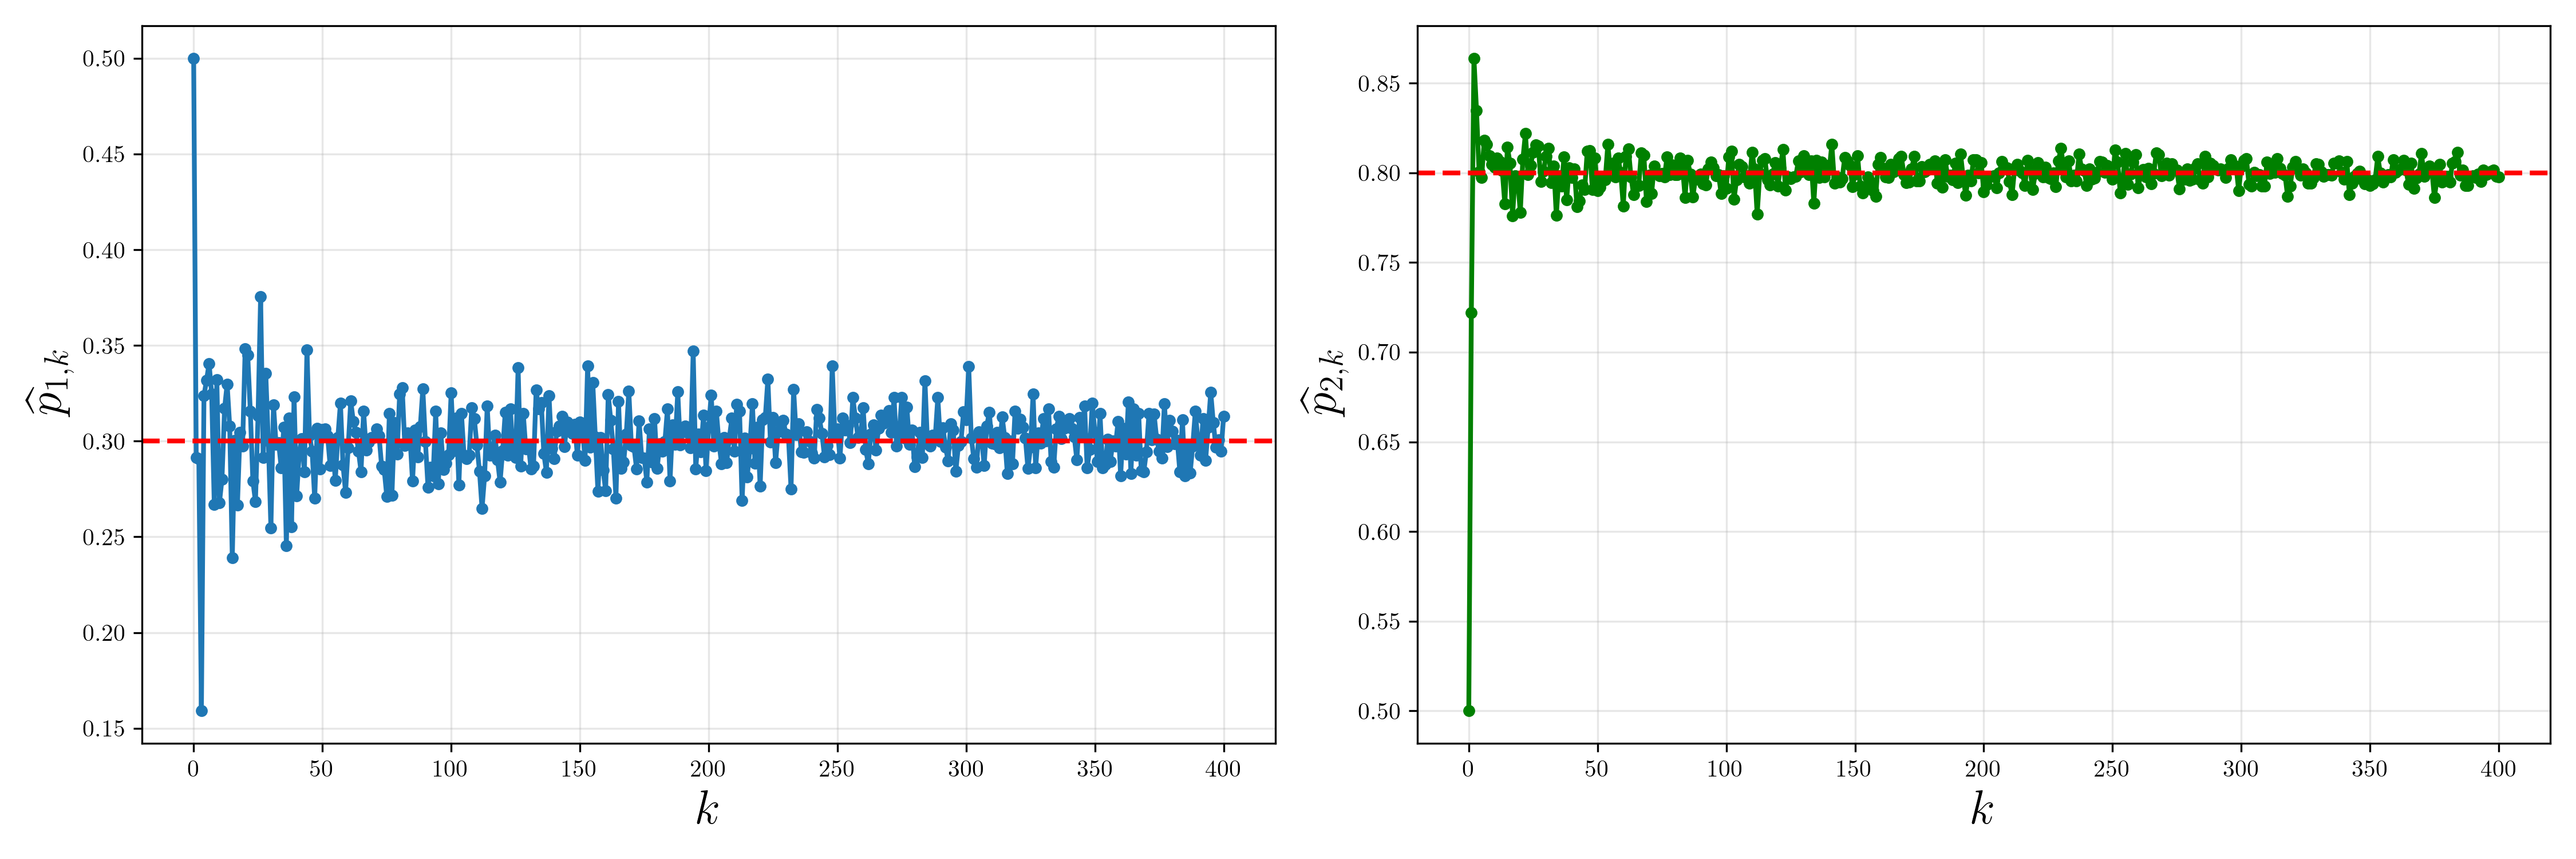
\includegraphics[width=0.85\textwidth]{Images/Algo 1/Example 1/convergence_plot.png}
        \caption{Plots of estimators $\widehat{p}_{1,k}$ and $\widehat{p}_{2,k}$ constructed after every iteration of the algorithm.}
        \label{fig:algo_1:example_1:estimator_convergence}
    \end{subfigure}

    \vspace{0.5cm} % adds some space between the two subfigures

    % Second subfigure
    \begin{subfigure}{\textwidth}
        \centering
        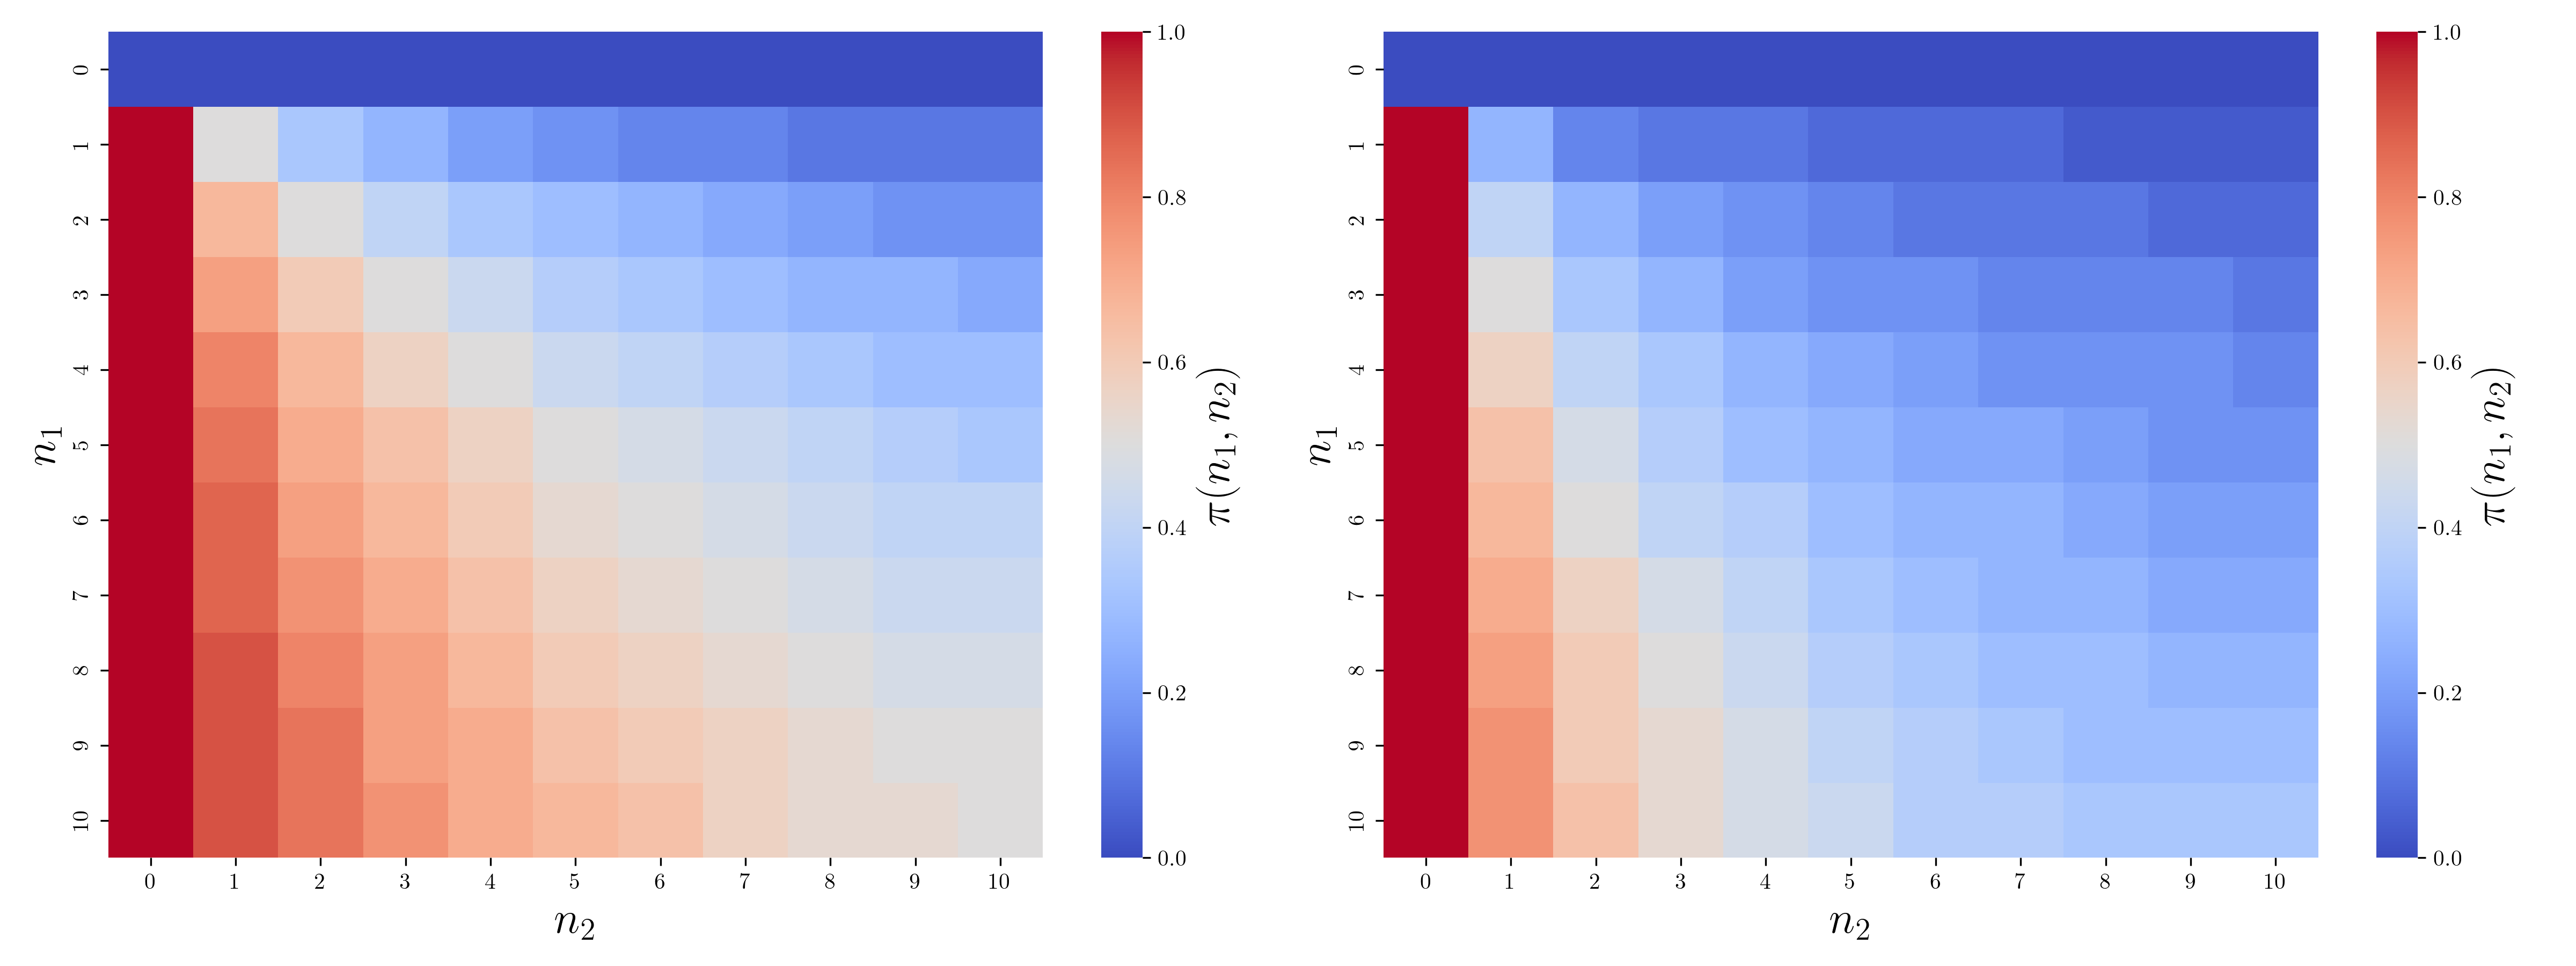
\includegraphics[width=0.85\textwidth]{Images/Algo 1/Example 1/policy_evolution.png}
        \caption{Heat maps of the policies at the start (left) and end (right).}
        \label{fig:algo_1:example_1:policy_evolution}
    \end{subfigure}

    \caption{Visualizations for Example 1}
    \label{fig:algo_1:example_1:combined}
\end{figure}




\begin{figure}[h]
    \centering
    % First subfigure
    \begin{subfigure}{\textwidth}
        \centering
        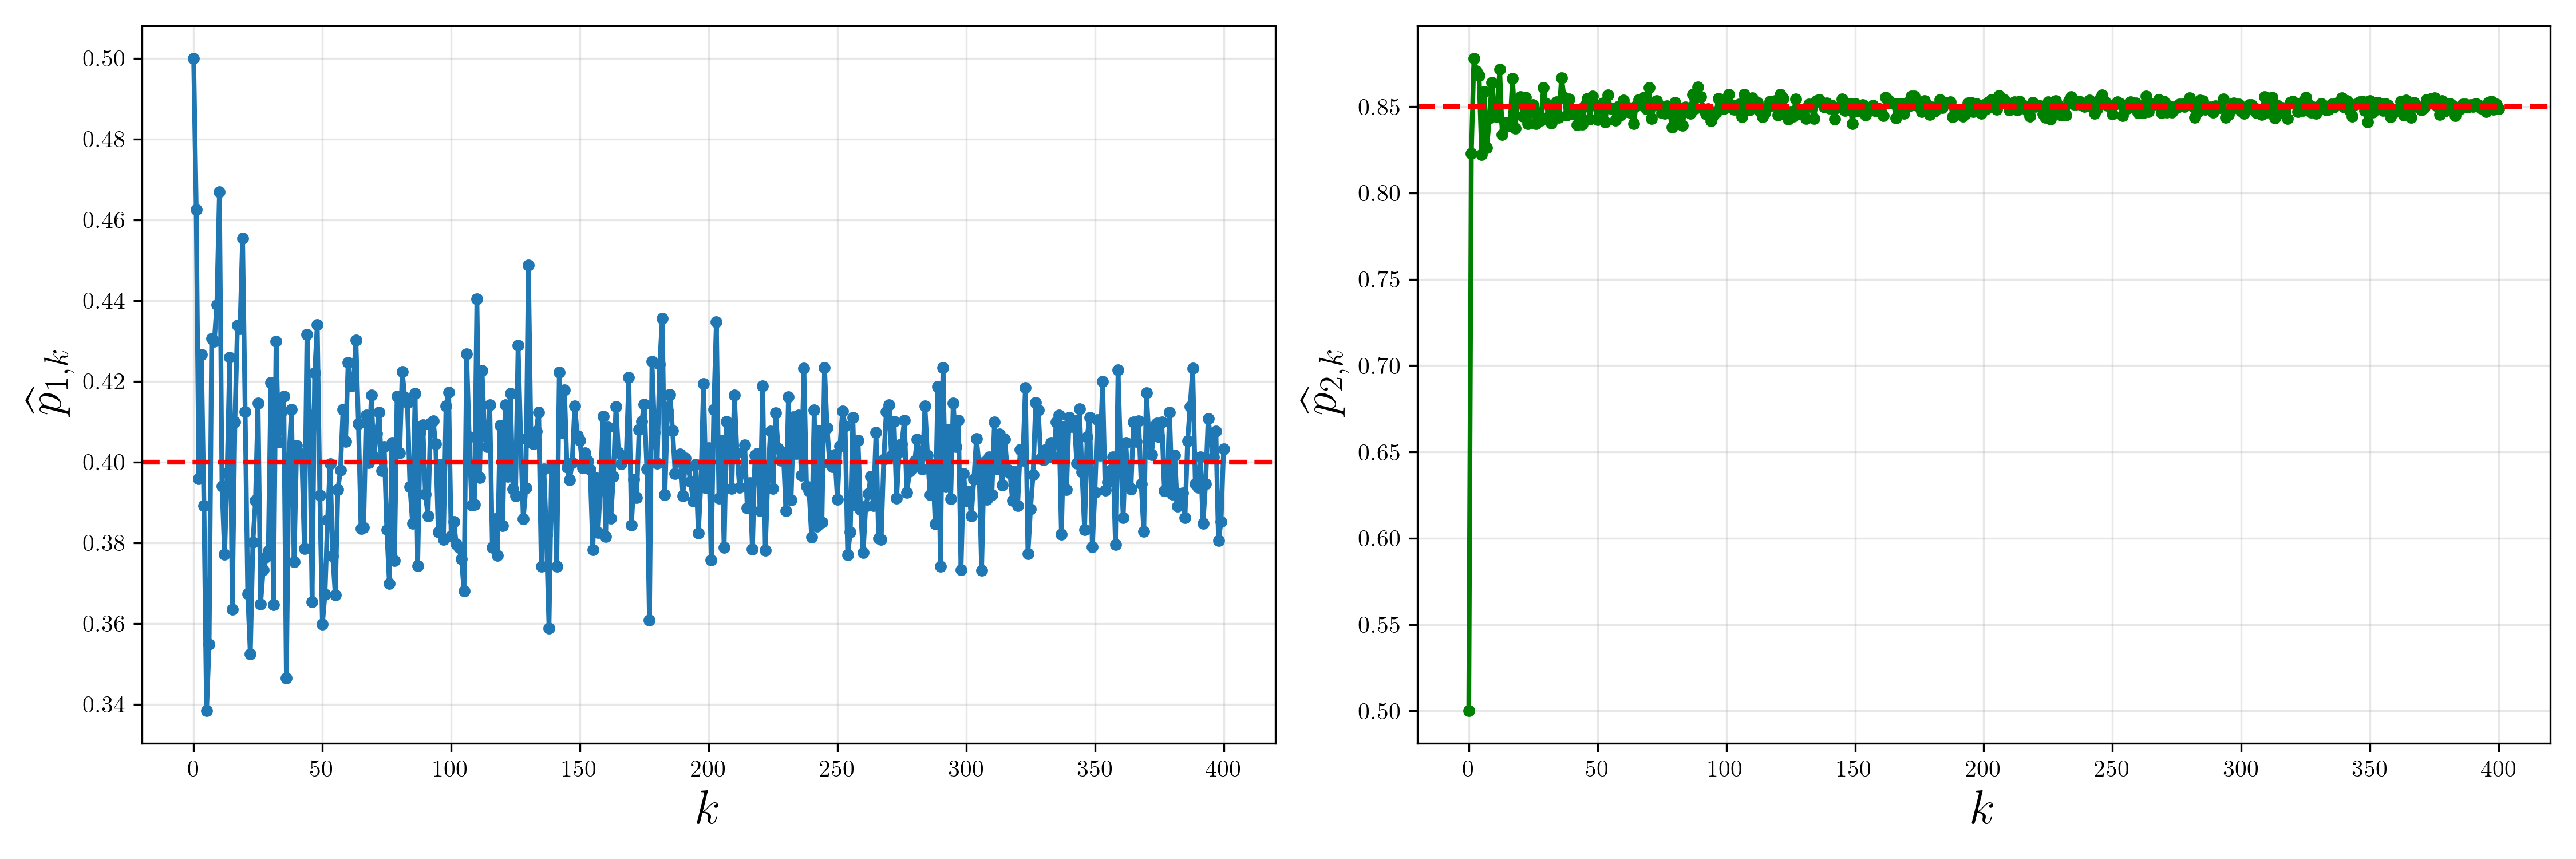
\includegraphics[width=0.85\textwidth]{Images/Algo 1/Example 2/convergence_plot.png}
        \caption{Plots of estimators $\widehat{p}_{1,k}$ and $\widehat{p}_{2,k}$ constructed after every iteration of the algorithm.}
        \label{fig:algo_1:example_2:estimator_convergence}
    \end{subfigure}

    \vspace{0.5cm} % adds some space between the two subfigures

    % Second subfigure
    \begin{subfigure}{\textwidth}
        \centering
        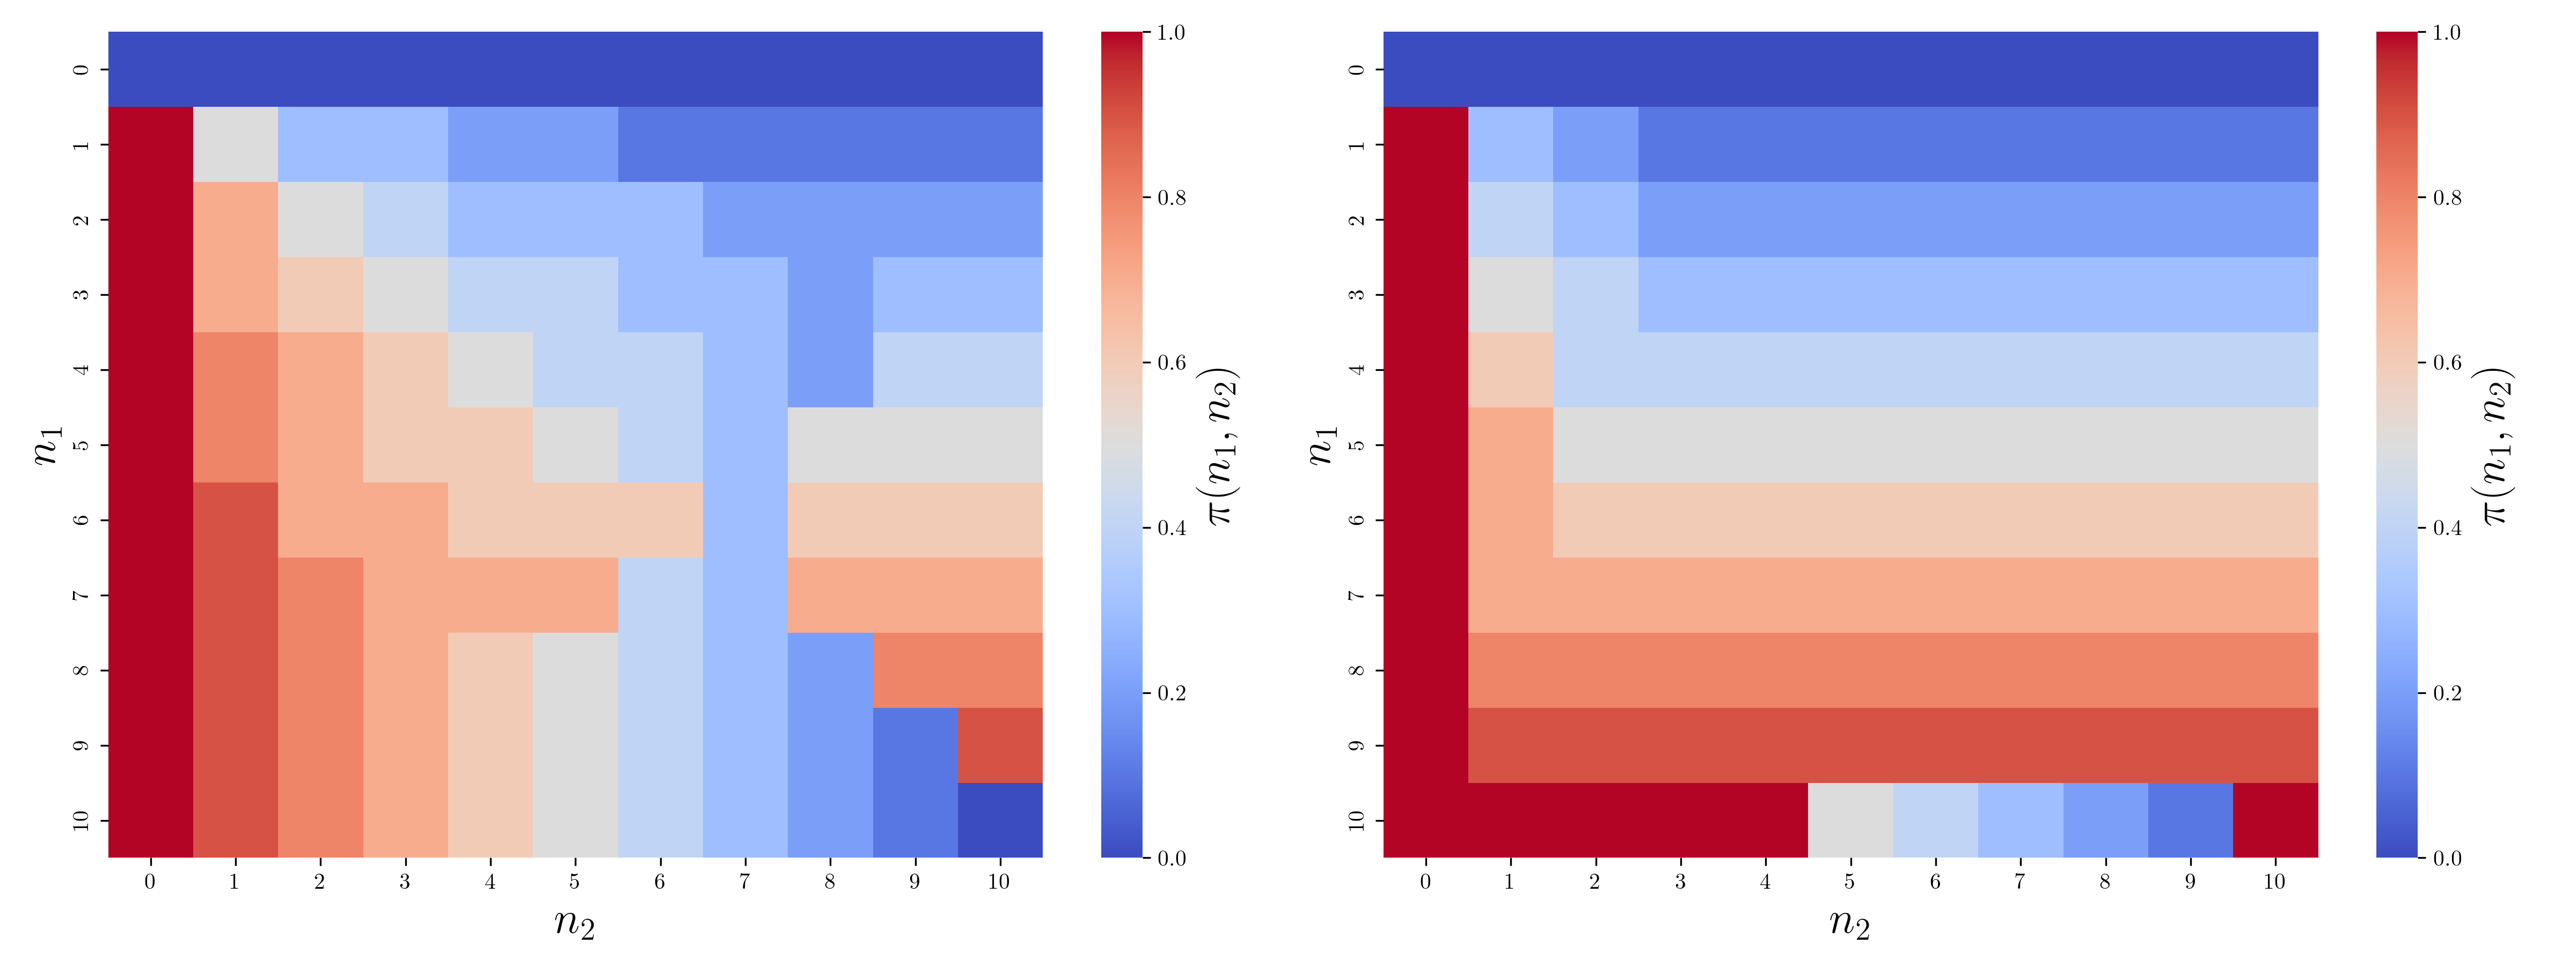
\includegraphics[width=0.85\textwidth]{Images/Algo 1/Example 2/policy_evolution.png}
        \caption{Heatmaps of the policies at the start (left) and end (right).}
        \label{fig:algo_1:example_2:policy_evolution}
    \end{subfigure}

    \caption{Visualizations for Example 2}
    \label{fig:algo_1:example_2:combined}
\end{figure}


We now investigate the performance of Algorithm \ref{alg: detailed learning algorithm} in a non-stationary setting, in which the parallelizability characteristics of an entire job class evolve over time. 
To capture this phenomenon, we consider an experiment in which the speed-up parameter of one job class changes at deterministic but unknown time epochs during the simulation horizon. The learning algorithm is not informed of these changes and must therefore adapt solely on the basis of newly observed inter-departure times. The aim of this experiment is to assess whether the estimation procedure is able to track the evolving degree of parallelizability, and whether the resulting allocation policy adjusts accordingly.
Figure \ref{fig:algo_1:example:changing_speed_up_parameter} illustrates the successful dynamic convergence of Algorithm \ref{alg: detailed learning algorithm} in this setting. The corresponding schedule of parameter changes is detailed in Table \ref{tab:parameter_schedule}, which specifies both the timing and magnitude of the shifts in the speed-up parameters.

\begin{figure}[h]
    \centering
    
    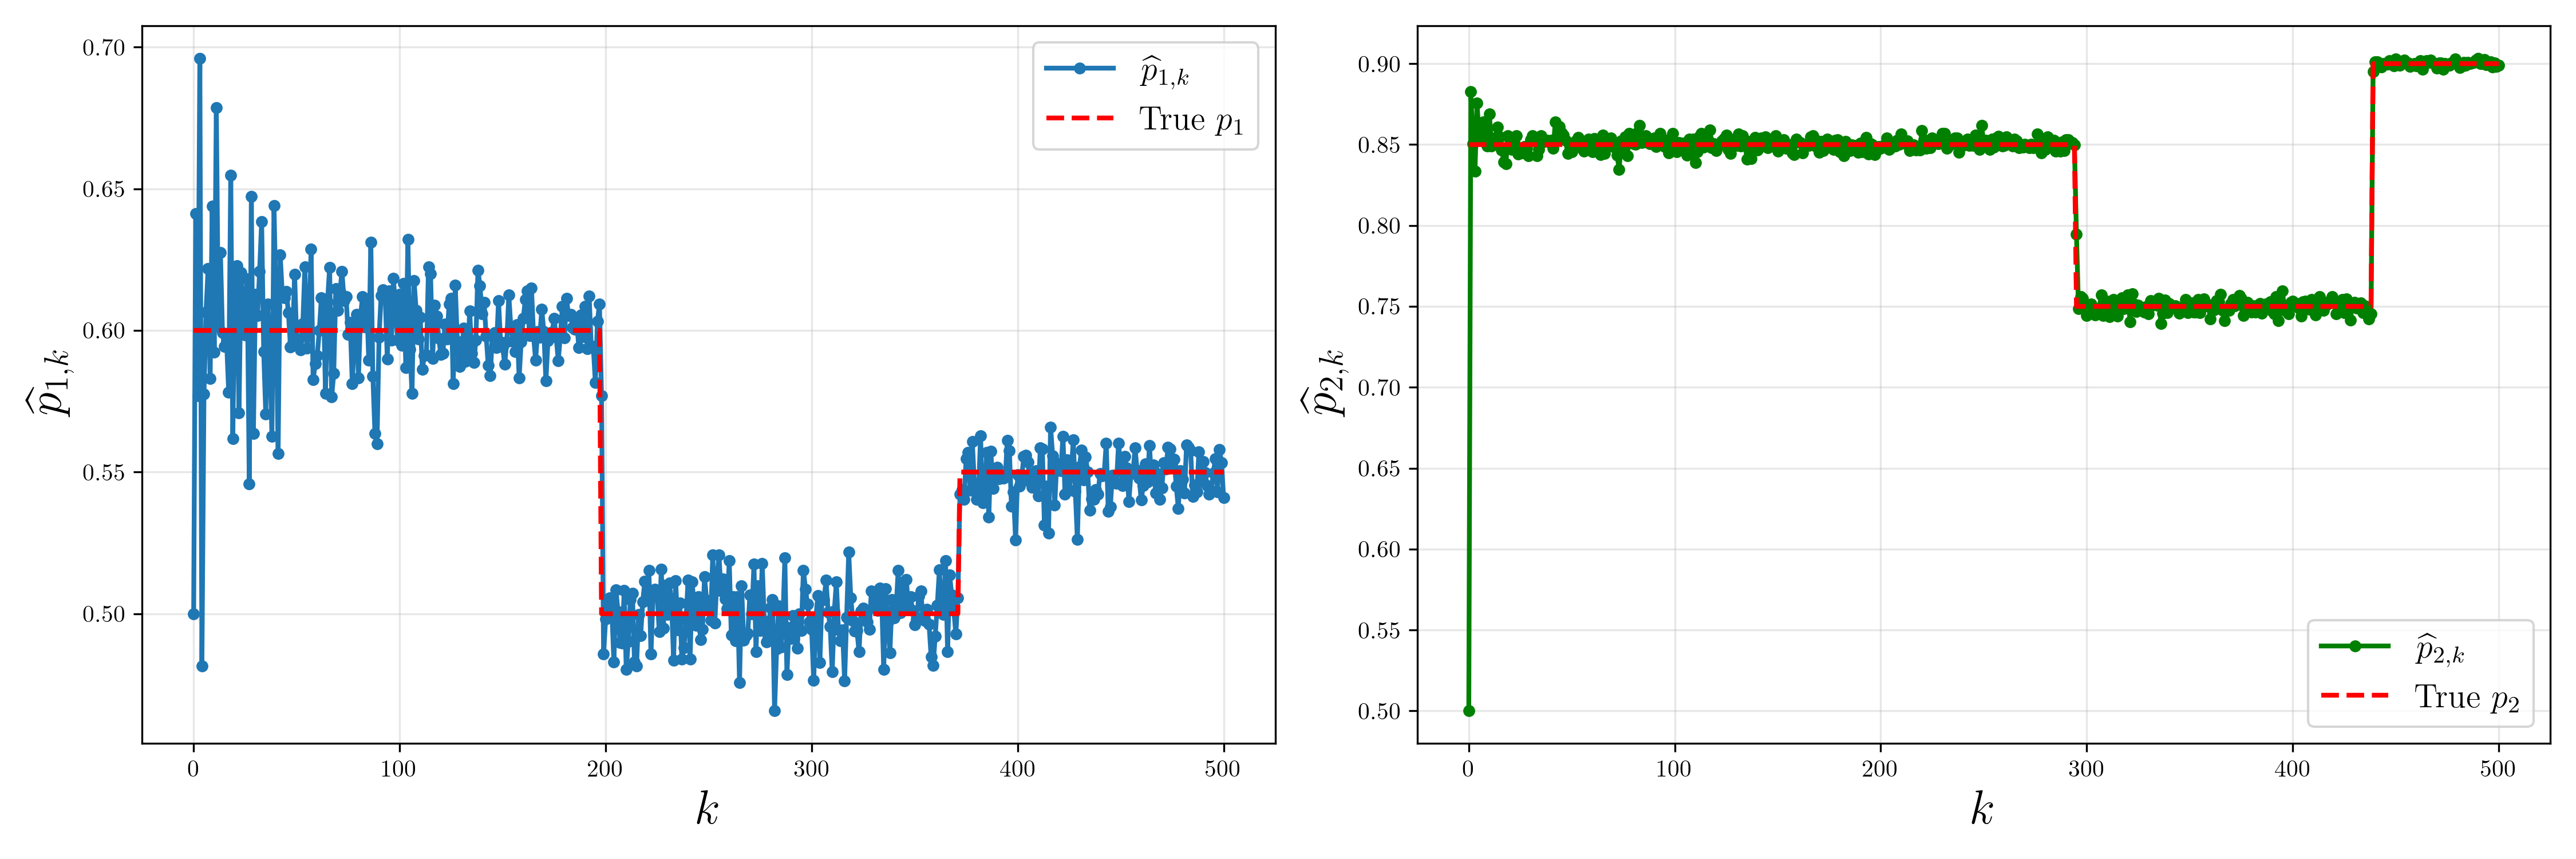
\includegraphics[width=0.85\textwidth]{Images/Algo 1/convergence_changing_p_time.png}
        
    \caption{A demonstration of the algorithm tracking a changing speed-up parameter.}
    \label{fig:algo_1:example:changing_speed_up_parameter}
\end{figure}

 


\begin{table}[htbp]
\centering
\caption{Parameter change schedule and corresponding simulation window information.}
\label{tab:parameter_schedule}
\begin{tabular}{ccccc}
\hline
Change point ($\times 10^5$) & $(p_1,p_2)$ & Iteration & \% through window \\
\hline

$t = 0$
& $(0.6,\,0.85)$
& 1
& $0\%$ \\

$t = 6$ 
& $(0.50,\,0.85)$ 
& 198 
& $87.2\%$ \\

$t = 12$ 
& $(0.50,\,0.75)$ 
& 295 
& $44.2\%$ \\

$t = 18$ 
& $(0.55,\,0.75)$ 
& 372 
& $46.0\%$ \\

$t = 24$ 
& $(0.55,\,0.90)$ 
& 439 
& $2.1\%$ \\

\hline
\end{tabular}
\end{table}

The first column specifies the time points at which the speed-up parameters change; in this experiment, these change points are chosen to be equidistant over the simulation horizon. The second column lists the corresponding values of the speed-up parameters after each change. For instance, the parameters are $(0.6, 0.85)$ on the interval $\big(0, 6\times10^5\big)$, and $(0.5, 0.85)$ on $\big(6\times10^5, 12\times10^5\big)$. The third column indicates the iteration number at which each parameter switch occurs. Finally, the fourth column reports the fraction of the corresponding time window that has elapsed at the moment of the change.
The remaining system parameters are given by $\lambda = 2$, $\mu = 1.5$, $c = 10$, $\alpha = 0.7$, and $N_k = 200\, k^{0.75}$.

% $M = 10$
% \footnote{\textcolor{blue}{LR: should this be $n_{max}$?}}



\subsection{Learning Algorithm 1b} \label{subsection: algorithm 2}

Recall that Theorem \ref{theorem:strong consistency} establishes strong consistency of the maximum likelihood estimates as size of the data increases, under the assumption that the core allocation policy is fixed.
In practice, we find that this assumption is quite restrictive, and strong consistency is observed also when the policy changes during the data generation process.
Leveraging this observation, in this section, we describe an alternative over Algorithm \ref{alg: improved detailed learning algorithm}, which leads to faster convergence when the speed-up parameter does not change with time.
% \footnote{\textcolor{blue}{LR: This is labeled as Algorithm 1b, but the subsection is Learning Algorithm 2. This causes some confusion also with later references.}}

\begin{algorithm}[H]
    \renewcommand{\thealgorithm}{1b}
    \caption{Improved learning algorithm}
    \label{alg: improved detailed learning algorithm}
    \begin{algorithmic}[1]
        \State Given: $\lambda, \mu, c, s(\cdot;p)$;
        \State Given: Choice of $N$, the number of departures in each epoch;
        \State Initialize policy $\pi_1$;
        \For{$k = 1,2,\dots, n_{\text{steps}}$}
        \State Run the system under policy $\pi_k$ during $\Big[\widetilde{T}_{k-1}, \widetilde{T}_k\Big)$ consisting of $N$ departures;
        \State Collect system sample path data in the entire interval $\Big[0, \widetilde{T}_k\Big)$ in the vector $\bs Z_k$;
        \State Compute the MLE $\big(\widehat{p}_{1,k},\widehat{p}_{2,k}\big)$;
        \State Compute $\pi_{k+1}$ using procedure of Section \ref{section: optimal policy} with parameters $\big(\widehat{p}_{1,k},\widehat{p}_{2,k}\big)$;
        \EndFor
        \State Output: $\pi_{n_{\text{steps}}+1}$;
    \end{algorithmic}
\end{algorithm}

In this variant of the algorithm, we fix a choice $N$ of the number of departures that will be observed in every epoch, i.e., for all $k$, the sequence $\big\{\widetilde{T}_k\big\}_{k \geq 1}$ is such that there are precisely $N$ departures in $\big[\widetilde{T}_{k-1}, \widetilde{T}_k\big)$.
Finally, the sample path data in the interval $\big[0, \widetilde{T}_k\big)$ consisting of $Nk$ departures is collected in the vector $\bs Z_k$ and is used to obtain estimators $\big(\widehat{p}_{1,k+1}, \ \widehat{p}_{2,k+1}\big)$. 
Similar to Algorithm~1, we then solve the Bellman optimality equation corresponding to these estimators to obtain policy $\widehat{\pi}_{k+1}$.

We now demonstrate the efficacy of Algorithm \ref{alg: improved detailed learning algorithm}  through Examples 3 and 4, as visualized in Figures \ref{fig:algo_2:example_1:combined} and \ref{fig:algo_2:example_2:combined}, respectively.
As remarked in Section \ref{subsection: algorithm 1}, once again because of quasi-identifiability issues, the convergence of estimators $\widehat{p}_{2,k}$ to $p_2$ is faster than that of estimators $\widehat{p}_{1,k}$ to $p_1$.

% \footnote{\textcolor{blue}{LR: Should this be 1b? Perhaps change the names of alogrithms.}}

\begin{figure}[h]
    \centering
    % First subfigure
    \begin{subfigure}{\textwidth}
        \centering
        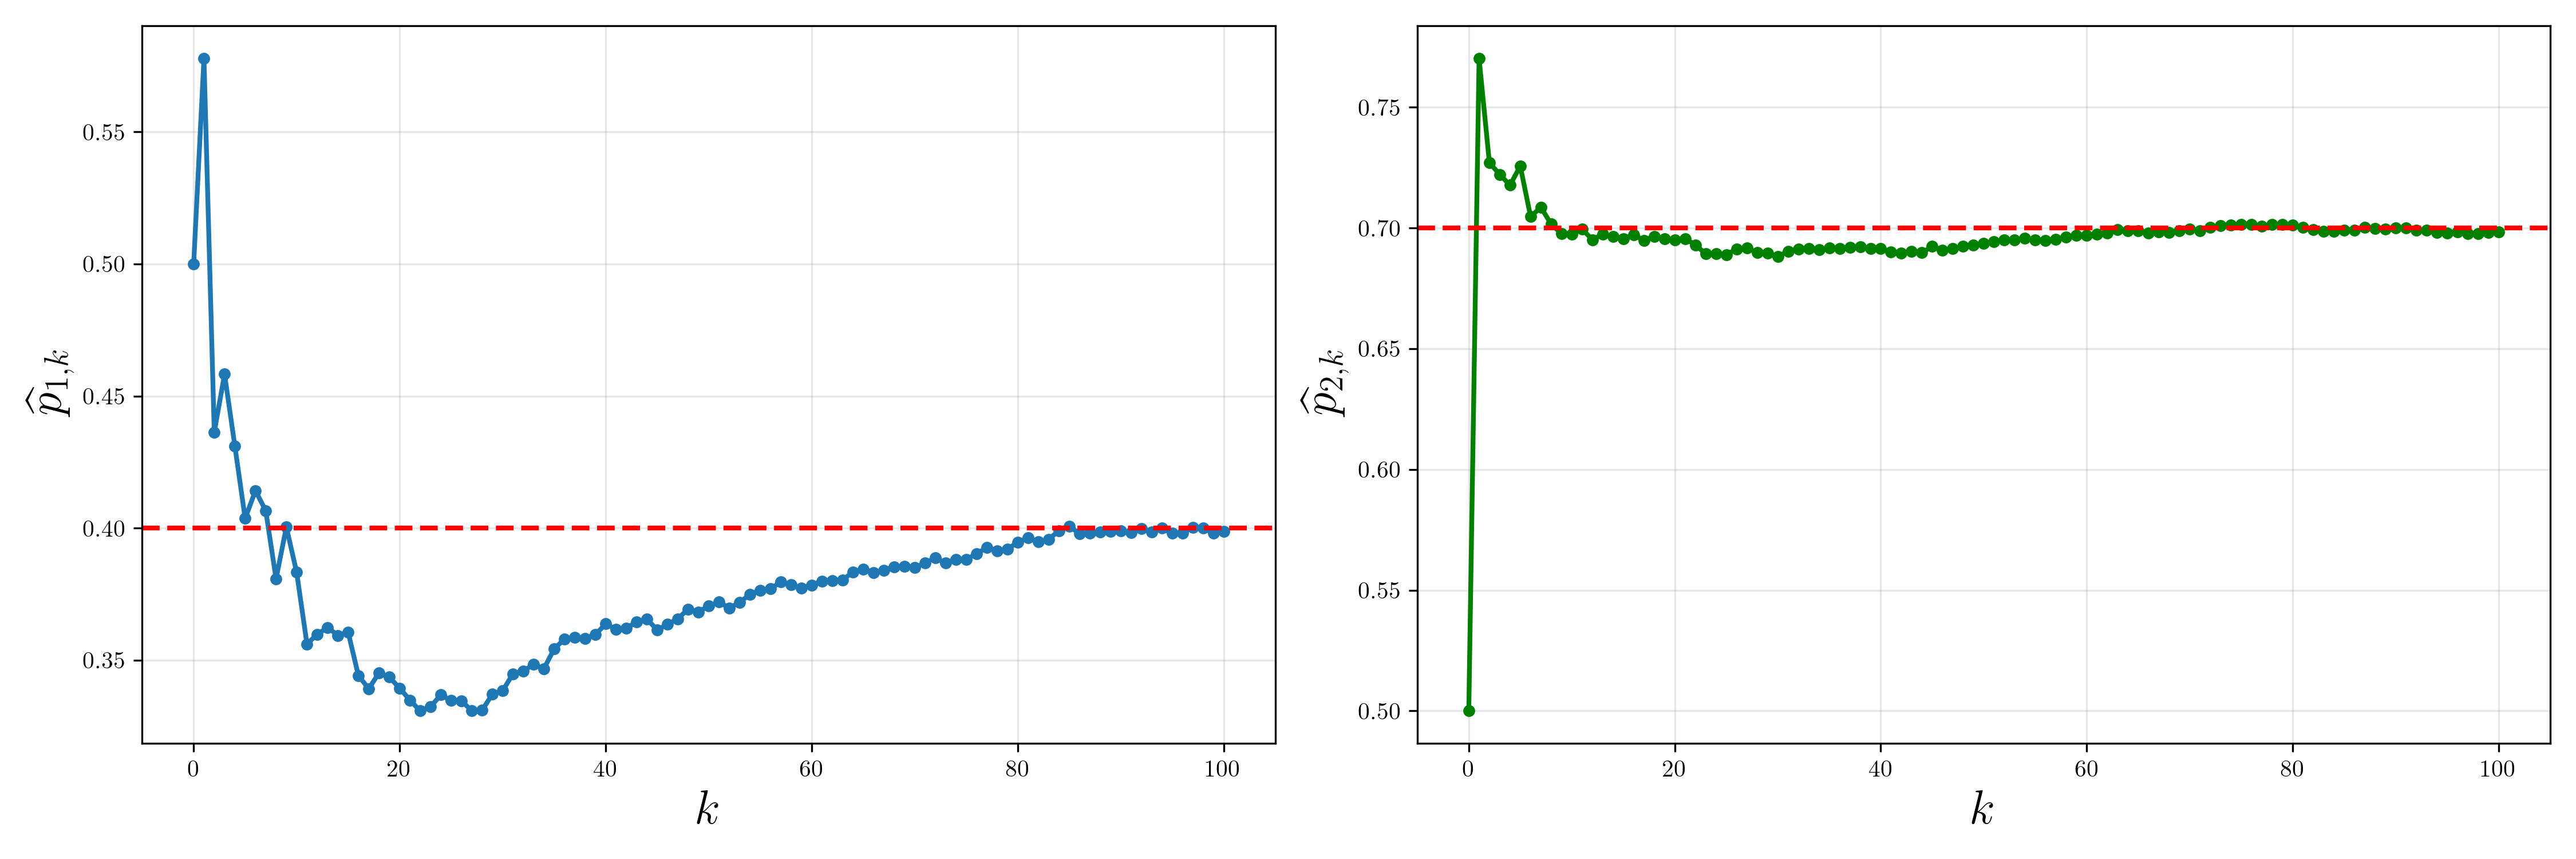
\includegraphics[width=0.85\textwidth]{Images/Algo 2/Example 1/convergence_plot.png}
        \caption{Plots of estimators $\widehat{p}_{1,k}$ and $\widehat{p}_{2,k}$ constructed after every iteration of the algorithm.}
        \label{fig:algo_2:example_1:estimator_convergence}
    \end{subfigure}

    \vspace{0.5cm} % adds some space between the two subfigures

    % Second subfigure
    \begin{subfigure}{\textwidth}
        \centering
        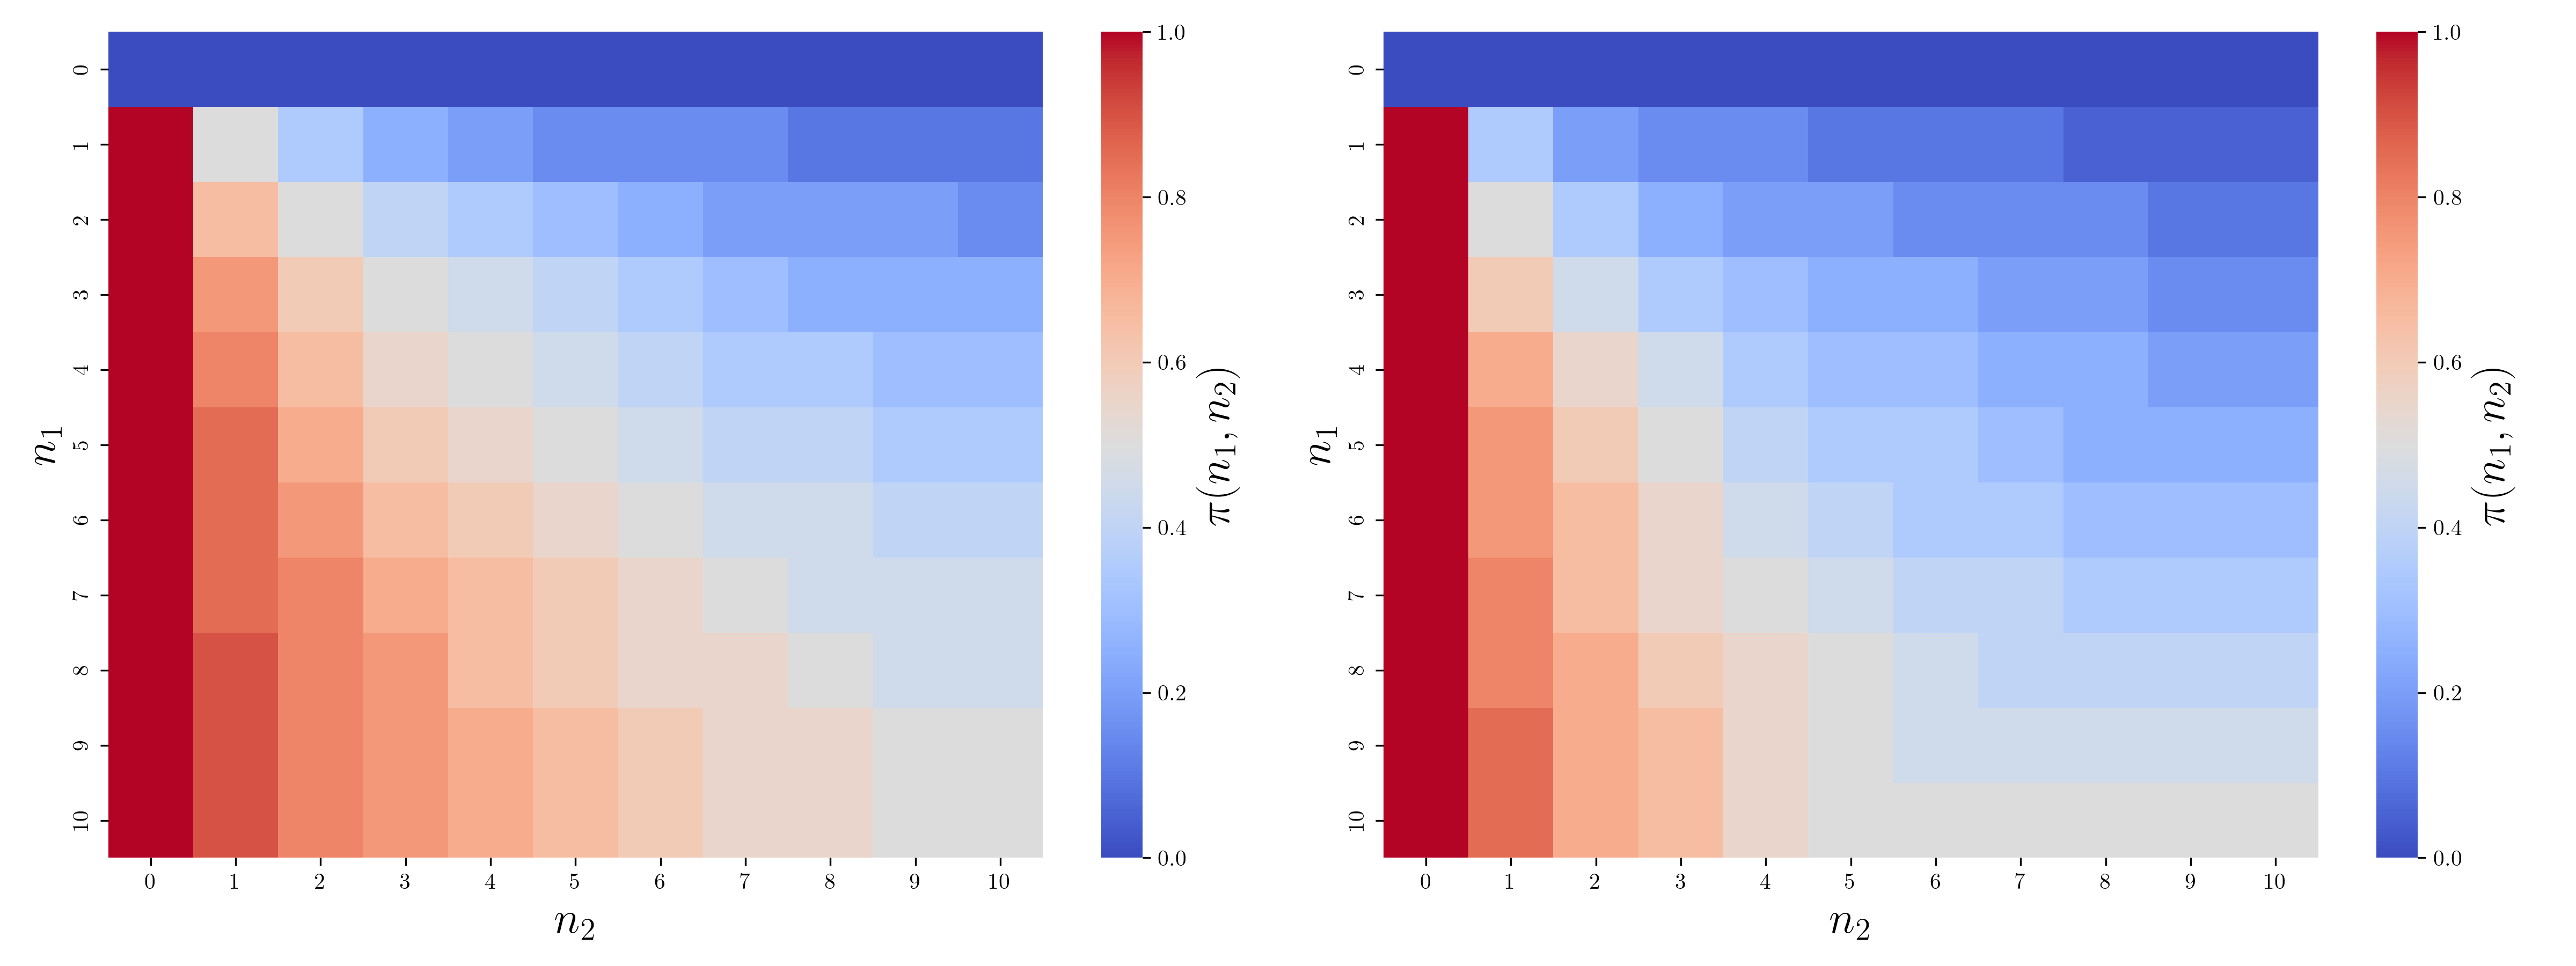
\includegraphics[width=0.85\textwidth]{Images/Algo 2/Example 1/policy_evolution.png}
        \caption{Heatmaps of the policies at the start (left) and end (right).}
        \label{fig:algo_2:example_1:policy_evolution}
    \end{subfigure}

    \caption{Visualizations for Example 3}
    \label{fig:algo_2:example_1:combined}
\end{figure}


\begin{figure}[h]
    \centering
    % First subfigure
    \begin{subfigure}{\textwidth}
        \centering
        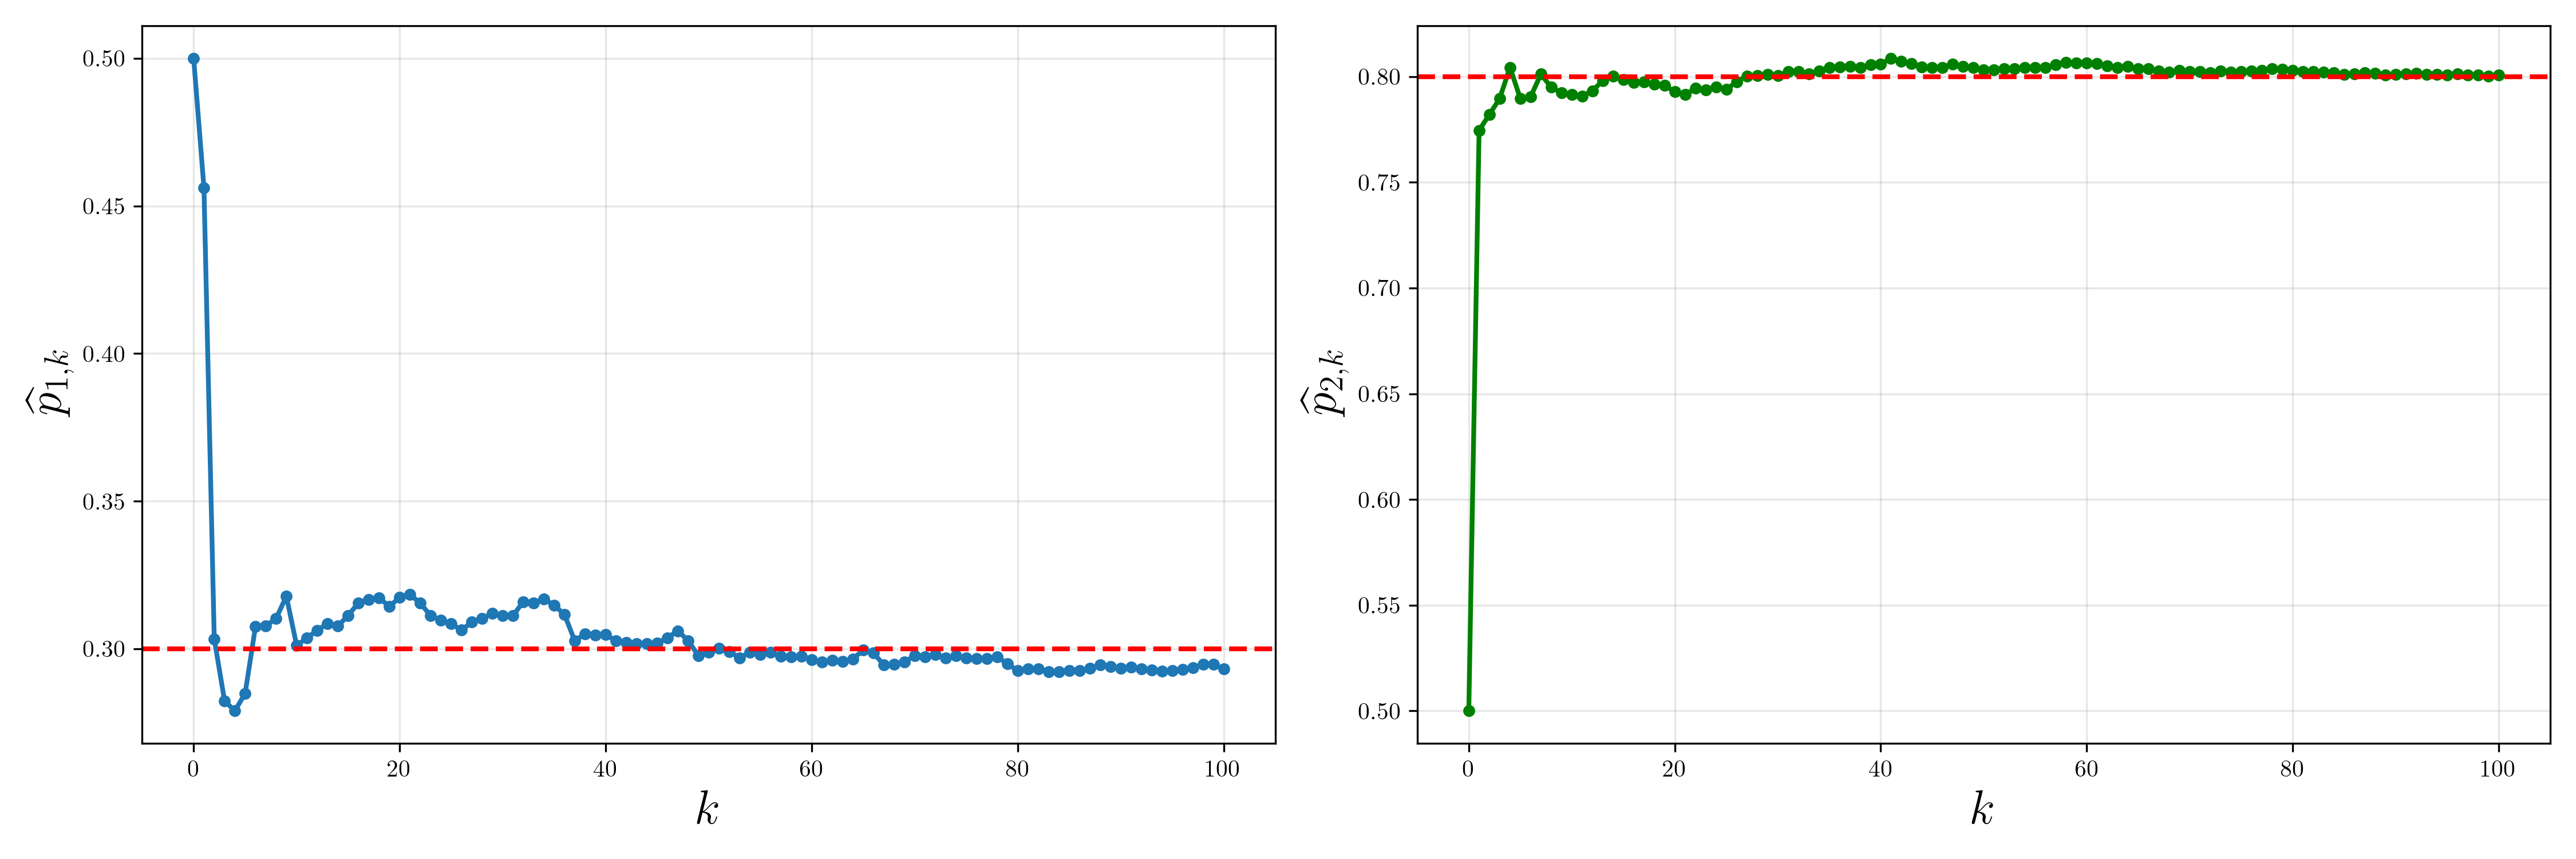
\includegraphics[width=0.75\textwidth]{Images/Algo 2/Example 2/convergence_plot.png}
        \caption{Plots of estimators $\widehat{p}_{1,k}$ and $\widehat{p}_{2,k}$ constructed after every iteration of the algorithm.}
        \label{fig:algo_2:example_2:estimator_convergence}
    \end{subfigure}

    \vspace{0.5cm} % adds some space between the two subfigures

    % Second subfigure
    \begin{subfigure}{\textwidth}
        \centering
        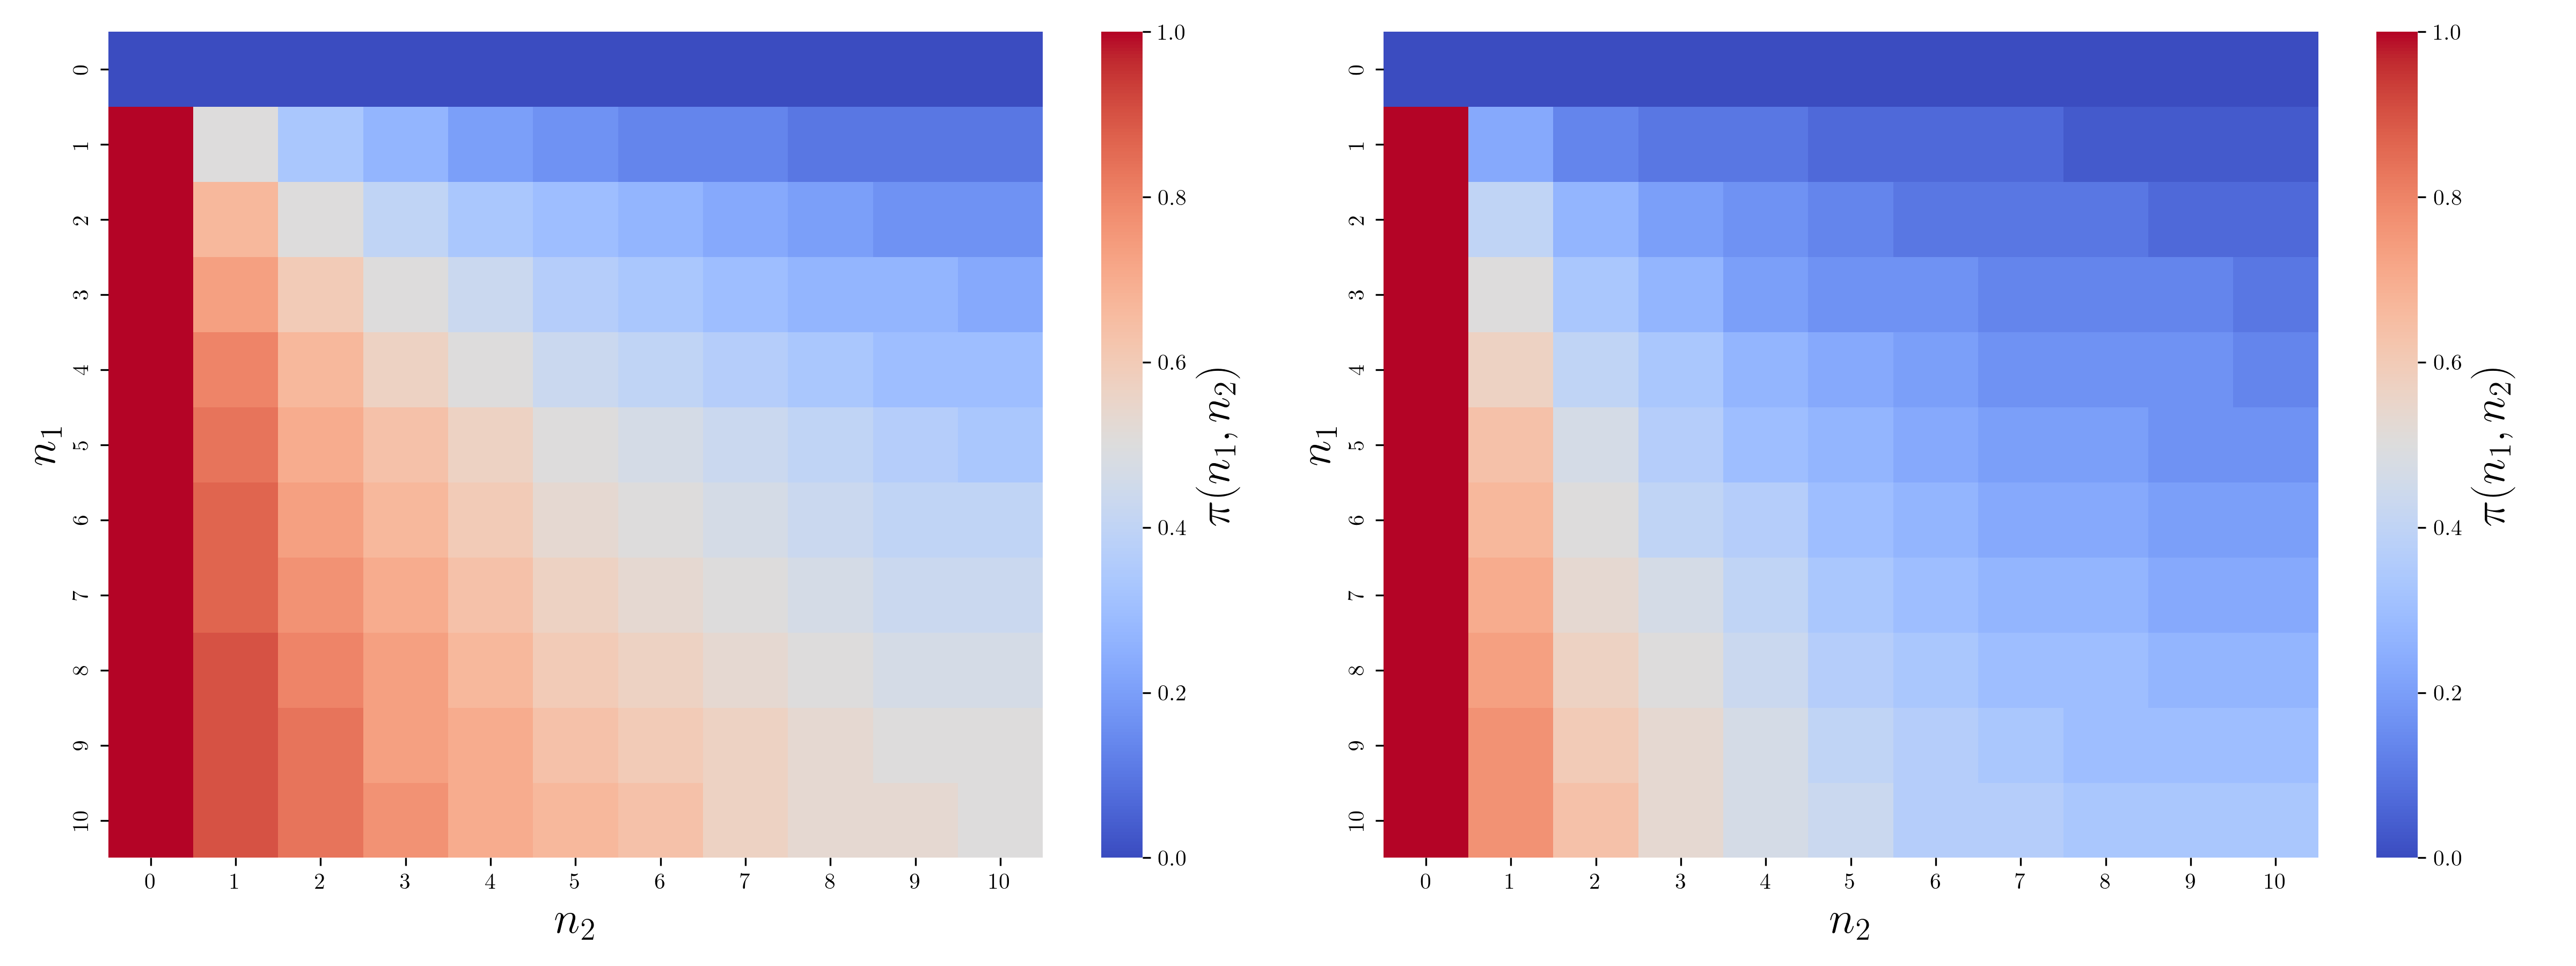
\includegraphics[width=0.75\textwidth]{Images/Algo 2/Example 2/policy_evolution.png}
        \caption{Heatmaps of the policies at the start (left) and end (right).}
        \label{fig:algo_2:example_2:policy_evolution}
    \end{subfigure}

    \caption{Visualizations for Example 4}
    \label{fig:algo_2:example_2:combined}
\end{figure}














\section{Conclusion}\label{section: conclusion}

% \footnote{\textcolor{red}{SAB: Open questions, extensions, closing remarks}}

In this paper, spurred in part by emerging applications such as the training of machine learning models, we studied the problem of dynamic resource allocation in a computing system with malleable jobs whose speed-up characteristics are not fully known a priori and may vary over time. Jobs belong to one of two observable classes, each characterized by an unknown degree of parallelizability. The objective is to learn a core-allocation policy that minimizes the long-run average sojourn time.

% To realize this goal, in this paper, we have provided an iterative estimation and optimization algorithm, where there is an interplay between enforcing a sub-optimal core allocation policy in order to collect data, and then using that data to refine the speed-up parameter estimators which subsequently refines the core allocation policy.
% An important intermediate step towards achieving this goal is to first learn the speed-up parameters corresponding to both job classes, for which, we developed a maximum likelihood estimation procedure on the observed inter-departure times.
% We also stated and proved a result which guarantees the strong consistency of the estimator to it's true value.

To address this problem, we developed an iterative learning-and-control framework that combines a statistical estimation step with an optimization step. At the core of our approach is a maximum likelihood estimation procedure based on observed inter-departure times, which enables online inference of the unknown speed-up parameters. These parameter estimates are then incorporated into a Markov decision process formulation to obtain updated resource-allocation policies. This yields a natural feedback loop between estimation and control: allocation decisions influence the observed data, while the resulting data are used to refine future decisions. We establish strong consistency of the proposed estimator, thereby providing theoretical support for the learning mechanism underlying the adaptive control scheme.

The framework developed in this paper extends naturally to systems with more than two job classes. While the estimation methodology remains essentially unchanged, the dimensionality of the control problem increases significantly, leading to substantial computational challenges in solving the associated Bellman optimality equations. This highlights an important tradeoff between model expressiveness and computational tractability in large-scale resource-allocation problems.

Finally, we outline several directions for future research. First, it would be of interest to study settings in which the speed-up characteristics evolve over time, reflecting non-stationary workloads or changing application behavior in modern cloud environments. Second, the current framework assumes exponential job sizes and Markovian dynamics; extending the analysis to more general service-time distributions is an important theoretical challenge. Finally, developing scalable approximation and reinforcement-learning-based methods for high-dimensional systems with many job classes remains a promising direction for future work.












































\bibliographystyle{plain}

{\small \begin{thebibliography}{10}

\bibitem{amazon2023}
Data Center Dynamics (2023).
\emph{Nvidia H100 GPUs now available on AWS}.
Available at {\small \url{https://www.datacenterdynamics.com/en/news/nvidia-h100-gpus-now-available-on-aws-as-amazons-cloud-scales-to-20000-gpu-clusters/}}.
Accessed: June 1, 2026.

\bibitem{amdahl1967}
Amdahl, G.
Validity of the single processor approach to achieving large scale computing capabilities.
In \textit{Proceedings of the April 18--20, 1967 Spring Joint Computer Conference}, 1967.

\bibitem{andrews1992}
Andrews, D.
Generic uniform convergence.
\textit{Econometric Theory} 8(2) (1992), 241--257.

\bibitem{armero1994bayesian}
Armero, C. and M.J. Bayarri.
Bayesian prediction in M/M/1 queues.
\textit{Queueing Systems} 15(1--4) (1994), 401--417.

\bibitem{asanjarani2021survey}
Asanjarani, A., Y. Nazarathy, and P. Taylor.
A survey of parameter and state estimation in queues.
\textit{Queueing Systems} 97(1) (2021), 39--80.

\bibitem{basawa2008}
Basawa, I.V., U.N. Bhat, and J. Zhou.
Parameter estimation using partial information with applications to queueing and related models.
\textit{Statistics \& Probability Letters} 78(12) (2008), 1375--1383.

\bibitem{berg2017}
Berg, B., J.L. Dorsman, and M. Harchol-Balter.
Towards optimality in parallel scheduling.
\textit{Proceedings of the ACM on Measurement and Analysis of Computing Systems} 1(2) (2017), 1--30.


\bibitem{berg2020}
Berg, B., R. Vesilo, and M. Harchol-Balter.
heSRPT: Parallel scheduling to minimize mean slowdown.
\textit{Performance Evaluation} 146 (2020), 102147.

 \bibitem{berg2022}
 Berg, B.
\textit{A Principled Approach to Parallel Job Scheduling}.
 PhD thesis, Carnegie Mellon University, 2022.

\bibitem{berg2024}
Berg, B., B. Moseley, W. Wang, and M. Harchol-Balter.
Asymptotically optimal scheduling of multiple parallelizable job classes.
\textit{arXiv preprint arXiv:2404.00346}, 2024.

\bibitem{bodas2023}
Bodas, S., M. Mandjes, and L. Ravner.
Statistical inference for a service system with non-stationary arrivals and unobserved balking.
\textit{arXiv preprint arXiv:2311.16884}, 2023.

\bibitem{cao2014}
Cao, Y., H. Sun, D. Qian, and W. Wu.
Scalable hierarchical scheduling for malleable parallel jobs on multiprocessor-based systems.
\textit{arXiv preprint arXiv:1412.4213}, 2014.

\bibitem{cera2010}
Cera, M., et al.
Supporting malleability in parallel architectures with dynamic CPUSETs mapping and dynamic MPI.
In \textit{Proceedings of the International Conference on Distributed Computing and Networking}, Springer, 2010.

\bibitem{chauhan2024}
Chauhan, N., et al.
A systematic literature review on task allocation and performance management techniques in cloud data centers.
\textit{arXiv preprint arXiv:2402.13135}, 2024.

\bibitem{chen1997}
Chen, H., O. Kella, and G. Weiss.
Fluid approximations for a processor-sharing queue.
\textit{Queueing Systems} 27(1--2) (1997), 99--125.

 \bibitem{cirne2001}
 Cirne, W. and F. Berman.
 A model for moldable supercomputer jobs.
 In \textit{Proceedings of the 15th International Parallel and Distributed Processing Symposium (IPDPS)}, 2001.

\bibitem{cirne2002}
Cirne, W. and F. Berman.
Using moldability to improve the performance of supercomputer jobs.
\textit{Journal of Parallel and Distributed Computing} 62(10) (2002), 1571--1601.


\bibitem{conttune2023}
Lian, J., et al.
ContTune: Continuous tuning by conservative Bayesian optimization for distributed stream data processing systems.
\textit{arXiv preprint arXiv:2309.12239}, 2023.

\bibitem{delimitrou2014}
Delimitrou, C. and C. Kozyrakis.
Quasar: Resource-efficient and QoS-aware cluster management.
\textit{ACM SIGPLAN Notices} 49(4) (2014), 127--144.

\bibitem{edmonds2000}
Edmonds, J.
Scheduling in the dark.
\textit{Theoretical Computer Science} 235(1) (2000), 109--141.

\bibitem{fernandez2024}
Fernandez, J., L. Wehrstedt, L. Shamis, M. Elhoushi, K. Saladi, Y. Bisk, E. Strubell, and J. Kahn.
Hardware scaling trends and diminishing returns in large-scale distributed training.
\textit{arXiv preprint arXiv:2411.13055}, 2024.


\bibitem{gonzalez2017}
Gonzalez, N., T. Carvalho, and C. Miers.
Cloud resource management: Towards efficient execution of large-scale scientific applications and workflows on complex infrastructures.
\textit{Journal of Cloud Computing} 6(1) (2017), 13.



\bibitem{google2024}
SiliconAngle.
Google Cloud turbocharges its AI hypercomputer stack with next-gen TPUs and bigger GPU clusters.
October 30, 2024.
Available at: {\small \url{https://siliconangle.com/2024/10/30/google-cloud-turbocharges-ai-hypercomputer-stack-next-gen-tpus-bigger-gpu-clusters/}}.
Accessed: June 1, 2026.

\bibitem{gupta2014}
Gupta, A., et al.
Towards realizing the potential of malleable jobs.
In \textit{Proceedings of the 21st International Conference on High Performance Computing (HiPC)}, 2014.

\bibitem{harchol-balter2021}
Harchol-Balter, M.
Open problems in queueing theory inspired by datacenter computing.
\textit{Queueing Systems} 97(1) (2021), 3--37.

\bibitem{hill2008}
Hill, M. and M. Marty.
Amdahl’s law in the multicore era.
\textit{Computer} 41 (2008), 33--38.

\bibitem{huang2013}
Huang, K.-C., T.-C. Huang, Y.-H. Tung, and P.-Z. Shih.
Effective processor allocation for moldable jobs with application speedup model.
In \textit{Advances in Intelligent Systems and Applications -- Volume 2},
Smart Innovation, Systems and Technologies, vol.\ 21. Springer, 2013, 563--572.

\bibitem{inoue2023}
Inoue, Y., L. Ravner, and M. Mandjes.
Estimating customer impatience in a service system with unobserved balking.
\textit{Stochastic Systems} 13(2) (2023), 181--210.

\bibitem{larson1990queue}
Larson, R.C.
The queue inference engine: Deducing queue statistics from transactional data.
\textit{Management Science} 36(5) (1990), 586--601.

\bibitem{li2024}
Li, Z., B. Berg, A. Mukhopadhyay, and M. Harchol-Balter.
How to rent GPUs on a budget.
In \textit{Proceedings of the 20th European Performance Engineering Workshop (EPEW)},
Lecture Notes in Computer Science, vol.\ 15454. Springer, Cham, 2024.

\bibitem{li2026}
Li, Z., M. Harchol-Balter, and B. Berg.
Mean field optimal core allocation across malleable jobs.
\textit{arXiv preprint arXiv:2602.01411}, 2026.

\bibitem{li2026-2}
Li, Z., C. Zhu, A. Mukhopadhyay, M. Harchol-Balter, and B. Berg.
BOA Constrictor: Squeezing performance out of GPUs in the cloud via budget-optimal allocation.
\textit{arXiv preprint arXiv:2602.01404}, 2026.

\bibitem{lym2019}
Lym, S., D. Lee, M. O'Connor, N. Chatterjee, and M. Erez.
DeLTA: GPU performance model for deep learning applications with in-depth memory system traffic analysis.
In \textit{Proceedings of the IEEE International Symposium on Performance Analysis of Systems and Software (ISPASS)}, IEEE, 2019, 293--303.

\bibitem{mccool2015}
McCool, M., A. Robison, and J. Reinders.
\textit{Structured Parallel Programming: Patterns for Efficient Computation}.
Morgan Kaufmann, 2015.

\bibitem{mckinsey2026}
McKinsey.
\textit{The cost of compute: A \$7 trillion race to scale data centers}.
{\small \url{https://www.mckinsey.com/industries/technology-media-and-telecommunications/our-insights/the-cost-of-compute-a-7-trillion-dollar-race-to-scale-data-centers/}}, accessed Jan.~11, 2026.

\bibitem{microsoft_article}
Microsoft.
\textit{Inside the world’s most powerful AI datacenter}.
{\small \url{https://blogs.microsoft.com/blog/2025/09/18/inside-the-worlds-most-powerful-ai-datacenter/}},
accessed Jan.~11, 2026.

\bibitem{puterman2014}
Puterman, M.~L.
\textit{Markov Decision Processes: Discrete Stochastic Dynamic Programming}.
John Wiley \& Sons, 2014.

\bibitem{podorojnyi2026estimating}
Podorojnyi, D. and L. Ravner.
Estimation of service value parameters for a queue with unobserved balking.
\textit{Queueing Systems} 110(2) (2026), Article 27.

\bibitem{ross2007estimation}
Ross, J.V., T. Taimre, and P.K. Pollett.
Estimation for queues from queue length data.
\textit{Queueing Systems} 55(2) (2007), 131--138.

\bibitem{shi2023}
Shi, J. and J. Lu.
Performance models of data parallel DAG workflows for large-scale data analytics.
\textit{Distributed and Parallel Databases} 41(3) (2023), 299--329.


\bibitem{whitt2006}
Whitt, W.
Fluid models for multiserver queues with abandonments.
\textit{Operations Research} 54(1) (2006), 37--54.

\bibitem{whitt2012fitting}
Whitt, W.
Fitting birth-and-death queueing models to data.
\textit{Statistics \& Probability Letters} 82(5) (2012), 998--1004.

\bibitem{wichelhaus2016nonparametric}
Antunes, N., G. Jacinto, A. Pacheco, and C. Wichelhaus.
Estimation of the traffic intensity in a piecewise-stationary M$_t$/G$_t$/1 queue with probing.
\textit{ACM SIGMETRICS Performance Evaluation Review} 44(2) (2016), 3--5.

\bibitem{zhang2009}
Zhang, J., J.~G. Dai, and B. Zwart.
Law of large number limits of limited processor-sharing queues.
\textit{Mathematics of Operations Research} 34(4) (2009), 937--970.

\bibitem{zhao2022}
Zhao, S., X. Dai, and I. Bate.
DAG scheduling and analysis on multi-core systems by modelling parallelism and dependency.
\textit{IEEE Transactions on Parallel and Distributed Systems} 33(12) (2022), 4019--4038.


\end{thebibliography}}






\end{document}